 %% Преамбула TeX-файла

% 1. Стиль и язык
\documentclass[utf8x]{G7-32} % Стиль (по умолчанию будет 14pt)
\usepackage[T2A]{fontenc}
\usepackage[russian]{babel}
\usepackage{setspace,lipsum}
\PassOptionsToPackage{shorthands=off}{babel}
\usepackage{bm}

\usepackage{mathtools}
\usepackage{caption}
\usepackage{subcaption}
\usepackage{verbatim}


\usepackage{pgfplots}
\pgfplotsset{compat=newest}
\usepackage{filecontents}
\usepackage{animate}
\usepackage{graphics}
\usepackage{color}
\def\alert#1{\textcolor{red}{#1}}

\usepgfplotslibrary{dateplot}
% Остальные стандартные настройки убраны в preamble.inc.tex.
\sloppy

% Настройки стиля ГОСТ 7-32
% Для начала определяем, хотим мы или нет, чтобы рисунки и таблицы нумеровались в пределах раздела, или нам нужна сквозная нумерация.
\EqInChapter % формулы будут нумероваться в пределах раздела
\TableInChapter % таблицы будут нумероваться в пределах раздела
\PicInChapter % рисунки будут нумероваться в пределах раздела

% Добавляем гипертекстовое оглавление в PDF
\usepackage[
bookmarks=true, colorlinks=true, unicode=true,
urlcolor=black,linkcolor=black, anchorcolor=black,
citecolor=black, menucolor=black, filecolor=black,
]{hyperref}

% Изменение начертания шрифта --- после чего выглядит таймсоподобно.
% apt-get install scalable-cyrfonts-tex

\IfFileExists{cyrtimes.sty}
    {
        \usepackage{cyrtimespatched}
    }
    {
        % А если Times нету, то будет CM...
    }

\usepackage{graphicx}   % Пакет для включения рисунков

% С такими оно полями оно работает по-умолчанию:
% \RequirePackage[left=20mm,right=10mm,top=20mm,bottom=20mm,headsep=0pt]{geometry}
% Если вас тошнит от поля в 10мм --- увеличивайте до 20-ти, ну и про переплёт не забывайте:
\geometry{right=20mm}
\geometry{left=30mm}


% Пакет Tikz
\usepackage{tikz}
\usetikzlibrary{arrows,positioning,shadows,shapes,patterns,spy,calc}
\usetikzlibrary{shapes.geometric}
\usetikzlibrary{decorations.markings}
%\usetikzlibrary{shapes.geometric,arrows.meta}


% Произвольная нумерация списков.
\usepackage{enumerate}

% ячейки в несколько строчек
\usepackage{multirow}

% itemize внутри tabular
\usepackage{paralist,array}


% Настройки листингов.
% 8 Листинги

\usepackage{listings}

% Значения по умолчанию
\lstset{
  basicstyle= \footnotesize,
  breakatwhitespace=true,% разрыв строк только на whitespacce
  breaklines=true,       % переносить длинные строки
%   captionpos=b,          % подписи снизу -- вроде не надо
  inputencoding=koi8-r,
  numbers=left,          % нумерация слева
  numberstyle=\footnotesize,
  showspaces=false,      % показывать пробелы подчеркиваниями -- идиотизм 70-х годов
  showstringspaces=false,
  showtabs=false,        % и табы тоже
  stepnumber=1,
  tabsize=4,              % кому нужны табы по 8 символов?
  frame=single
}

% Стиль для псевдокода: строчки обычно короткие, поэтому размер шрифта побольше
\lstdefinestyle{pseudocode}{
  basicstyle=\small,
  keywordstyle=\color{black}\bfseries\underbar,
  language=Pseudocode,
  numberstyle=\footnotesize,
  commentstyle=\footnotesize\it
}

% Стиль для обычного кода: маленький шрифт
\lstdefinestyle{realcode}{
  basicstyle=\scriptsize,
  numberstyle=\footnotesize
}

% Стиль для коротких кусков обычного кода: средний шрифт
\lstdefinestyle{simplecode}{
  basicstyle=\footnotesize,
  numberstyle=\footnotesize
}

% Стиль для BNF
\lstdefinestyle{grammar}{
  basicstyle=\footnotesize,
  numberstyle=\footnotesize,
  stringstyle=\bfseries\ttfamily,
  language=BNF
}

% Определим свой язык для написания псевдокодов на основе Python
\lstdefinelanguage[]{Pseudocode}[]{Python}{
  morekeywords={each,empty,wait,do},% ключевые слова добавлять сюда
  morecomment=[s]{\{}{\}},% комменты {а-ля Pascal} смотрятся нагляднее
  literate=% а сюда добавлять операторы, которые хотите отображать как мат. символы
    {->}{\ensuremath{$\rightarrow$}~}2%
    {<-}{\ensuremath{$\leftarrow$}~}2%
    {:=}{\ensuremath{$\leftarrow$}~}2%
    {<--}{\ensuremath{$\Longleftarrow$}~}2%
}[keywords,comments]

% Свой язык для задания грамматик в BNF
\lstdefinelanguage[]{BNF}[]{}{
  morekeywords={},
  morecomment=[s]{@}{@},
  morestring=[b]",%
  literate=%
    {->}{\ensuremath{$\rightarrow$}~}2%
    {*}{\ensuremath{$^*$}~}2%
    {+}{\ensuremath{$^+$}~}2%
    {|}{\ensuremath{$|$}~}2%
}[keywords,comments,strings]

% Подписи к листингам на русском языке.
\renewcommand\lstlistingname{\cyr\CYRL\cyri\cyrs\cyrt\cyri\cyrn\cyrg}
\renewcommand\lstlistlistingname{\cyr\CYRL\cyri\cyrs\cyrt\cyri\cyrn\cyrg\cyri}

\definecolor{codegreen}{rgb}{0,0.6,0}
\definecolor{codegray}{rgb}{0.5,0.5,0.5}
\definecolor{codepurple}{rgb}{0.58,0,0.82}
\definecolor{backcolour}{rgb}{0.95,0.95,0.92}

\lstdefinestyle{mystyle}{
    backgroundcolor=\color{backcolour},   
    commentstyle=\color{codegreen},
    keywordstyle=\color{magenta},
    numberstyle=\tiny\color{codegray},
    stringstyle=\color{codepurple},
    basicstyle=\ttfamily\footnotesize,
    breakatwhitespace=false,         
    breaklines=true,                 
    captionpos=b,                    
    keepspaces=true,                 
    numbers=left,                    
    numbersep=5pt,                  
    showspaces=false,                
    showstringspaces=false,
    showtabs=false,                  
    tabsize=2
}

\lstset{style=mystyle}


% Полезные макросы листингов.
% Любимые команды
\newcommand{\Code}[1]{\textbf{#1}}


\begin{document}

\thispagestyle{empty}

\newgeometry{top=2cm,bottom=2cm,left=3cm,right=1cm}
{
\singlespacing
\begin{center}
ФГБОУ ВО <<Московский государственный университет имени~М.~В.~Ломоносова>>
\medskip
\hrule
\medskip
Механико-математический факультет
\end{center}

\vspace{20mm}
\begin{flushright}
На правах рукописи

%{\sl УДК 519.713.3}
\end{flushright}

\vspace{25mm}
\begin{center}
{\large Рязанов Даниил Александрович}
\end{center}

\vspace{5mm}
\begin{center}
{\bf \large Бигармонические аттракторы внутренних волн 
\par}

\vspace{10mm}
{
01.02.05~--- Механика жидкости газа и плазмы
}

%\parbox{0.88\textwidth}{
%Специальность 05.13.17~---
%Теоретические основы информатики
%}
%\parbox{0.88\textwidth}{
%\vspace{5mm}
%Специальность 05.13.19~---
%Методы и системы защиты информации,
%}
%информационная безопасность

%\begin{tabular}{r c l}
%Специальность 05.13.17& --- &Теоретические основы информатики\\[3mm]
%Специальность 05.13.19& --- &\parbox[t]{10cm}{Методы и системы защиты информации,\\ \centering информационная безопасность}
%\end{tabular}



\vspace{10mm}
Научно-квалификационная работа
\end{center}

\vspace{16mm}
\begin{flushright}
Научный руководитель:\\[2mm]
д.ф.-м.н., \\
Веденеев~В.\,В.\\

\end{flushright}

\vfill
\begin{center}
{Москва -- 2020}
\end{center}
}
\newpage
\restoregeometry

\frontmatter % выключает нумерацию ВСЕГО; здесь начинаются ненумерованные главы: реферат, введение, глоссарий, сокращения и прочее.

% Команды \breakingbeforechapters и \nonbreakingbeforechapters
% управляют разрывом страницы перед главами.
% По-умолчанию страница разрывается.

% \nobreakingbeforechapters
% \breakingbeforechapters

\tableofcontents

\Introduction

Внутренние волны возникают в стратифицированных жидкостях между слоями различной плотности. Самым распространенным примером стратифицированной жидкости является океан.  Внутренние волны распространяются согласно дисперсионному закону \cite{MowbrayRarity1967}, которое связывает частоту волн и угол наклона волнового пучка по отношению к вектору силы тяжести, но не содержит масштаба длины. 

Подчиняясь дисперсионному соотношению внутренние волны при отражении от наклонных поверхностях могут фокусироваться. Под фокусировкой подразумевается увеличивающуюся амплитуду колебаний стратифицированной жидкости. При определенных геометрически параметрах морского дна или резервуара со стратифицированной жидкостью после многократных отражений внутренние волны начинают циркулировать по замкнутой траектории. На этой траектории наблюдается многократное увеличение амплитуды колебаний, а сама траектория называется аттрактором внутренних волн.

Аттракторы в океанах оказывают влияние на процессы перемешивания, перераспределение кинетической энергии между течениями различных масштабов, осаждения примесей, динамику спускаемых аппаратов и миграцию живых организмов. Это обуславливает \textbf{актуальность} изучения явления аттракторов внутренних гравитационных волн.

Важной задачей изучения аттракторов внутренних волн с помощью численных методов является обеспечение возможности проводить численные эксперименты с геометрией, приближенной к геометрии реального дна океана. Выполнение этой задачи ускорило и удешевило бы процесс непосредственного поиска аттракторов внутренних волн в океане, и изучение влияния аттркаторов на турбулентные режимы течения в водоемах. Метод спектральных элементов, который обеспечивает достаточную точность воспроизведения результатов эксперимента, ограничен в своей реализации сложностью геометрии расчетной области. В свою очередь, метод конечного объема позволяет работать со сложной геометрией, которая способна имитировать поверхность океанического дна, но стандартные реализации не обладают достаточной точностью для количественного воспроизведения эксперимента. Кроме того, монохроматический источника возмущений может не описывать реальные внешние воздействия. Зачастую, при моделировании явлений, связанных с образованием аттракторов в реальных условиях, необходимо учитывать несколько приливных воздействий \cite{Garrett1972} и изменение стратификации.

 

\paragraph{Цель работы} -- изучение явления бигармонического аттрактора, которое возникает при воздействии на стратифицированную жидкость двухчастотным волнопродуктором.  
С этой целью были поставлены следующие задачи \textbf{задачи}:

\begin{itemize}

  \item Нахождение интервала частот внешних воздействий, при которых возникает аттрактор внутренних волн.
  
  % Изучение интервалов частот внешних воздействий и других параметров, при которых происходит аккумуляция волновой энергии, в частности волновых аттракторов.

%    \item Нахождение частотных параметров приводящих к образованию аттракторов в резервуаре.
    
  % \item Обзор существующих методов моделирования аттракторов внутренних волн. Выявление их достоинств и недостатков.
    
  \item Реализация численных экспериментов с помощью двух подходов: спектрально-элементного и конечно-объемного.

  \item Разработка новой программы для моделирования аттракторов внутренних волн на основе квазигидродинамического подхода.
    
  \item Верификация результатов численного моделирования.

  \item Описание особенностей волновых режимов при бигармоническом воздействии и значительно отличающихся частотах воздействия и малых амплитудах.

  \item Описание особенностей волновых режимов при бигармоническом воздействии, близких частотах воздействия и малых амплитудах.
    
  \item Описание особенностей нелинейных волновых режимов при бигармоническом воздействии и близких частотах воздействия.

  \item Сравнение динамики средней кинетической энергии и пульсации кинетической энергии для монохроматического режима и различных бигармонических режимов.
    

    
\end{itemize}

\paragraph{Методы решения поставленных задач}

Для решения поставленных задач были использованы методы математического моделирования механики сплошных сред, такие как метод спектральных элементов и метод конечного объема. Для предсказания формы аттрактора внутренних волн использовался метод трассировки лучей. Для анализа данных использовался метод построения частотно-временных диаграмм при помощи быстрого преобразования Фурье.

\paragraph{Научная новизна работы} выражается в конкретных результатах:
\begin{enumerate}[1.]
  \item Получены аналитические выражения для границ частотного интервала существования аттракторов внутренних волн.% конфигурации (1,1). 
    
  \item Получена геометрия течения, которая возникает в трапециевидном резервуаре, наполненном стратифицированной жидкостью при воздействии на жидкость внешними возмущениями с двумя различными частотами. 
    
  \item Проведён анализ результатов моделирования аттрактора внутренних волн при бигармоническом воздействии, полученных с помощью метода спектральных элементов. Для различных комбинаций возмущающих частот построен спектр, частотно-временная диаграмма и зависимость средней кинетической энергии от времени. 
    
  \item Реализован квазигидродинамический подход на базе метода конечного элемента. Проведено сопоставление результатов моделирования методов конечных объемов и методом спектральных элементов.
\end{enumerate}

\paragraph{Достоверность результатов}

Достоверность полученных результатов гарантируется строгой математической постановкой, верификацией и валидацией разработанного алгоритма для решения поставленной задачи.

% \paragraph{Объектом исследования} являются волновые режимы возникающие %в естественных условиях 
% при двух источниках внешних воздействий на стратифицированную жидкость в трапециевидном резервуаре.

% %Приложения включают в себя задачи океанологии, астрофизики и технических вращающихся систем при периодических воздействиях. 

% %\paragraph{В исследовании использованы следующие методы:}
% \begin{itemize}
%   \item [    В исследовании использованы \textbf{
% методы:}]
%   \item методы численного моделирования конечного объема;
%   \item метод спектральных элементов;
%   \item метод трассировки лучей;
%   \item Фурье анализ полученных результатов, в том числе по скользящему окну;
%   \item разложение по эмпирическим модам;
% \end{itemize}

% % В работе рассматриваются резервуары в форме трапеций различных конфигураций, заполненных стратифицированной жидкостью. Одна из стенок резервуара представляет собой волнопродуктор, который порождает внутренние волны в стратифицированной среде. Результаты разработки предоставляют возможность проводить моделирование аттракторов внутренних волн в условиях сложной геометрии и неортогональных сетках. 



\paragraph{Практическая значимость} 

Ранее эксперименты по исследованию бигармонических аттракторов, как численные так и натурные, не проводились. Теоретически, бигармонический аттрактор представляет собой новую устойчивую структуру, которая образуется в стратифицированной жидкости при воздействии на нее периодическим двухчастотным возмущением.

Положения и выводы диссертационного исследования могут быть использованы для подбора параметров  волнового аттрактора в лабораторных условиях или при численном моделировании. Среди возможных приложений результатов работы — задачи моделирования аттракторов внутренних волн на сложных геометриях, задачи моделирования течений со сложным спектром частотных воздействий на стратифицированную жидкость. Работа является первым шагом к моделированию течений, возникающих в условиях, приближенных к реальным океаническим, что позволит выяснить форму и вид природных аттракторов внутренних волн. Комбинация методов конечного объёма и квазигидродинамических уравнений позволила добиться существенного улучшения в точности моделирования и дала инструмент к  усложнению геометрии расчётной области. Разработанная программа может быть применена не только к задачам моделирования аттрактора, но и к другим задачам гидродинамики с дозвуковыми и трансзвуковыми скоростями.

\paragraph{На защиту выносятся следующие положения:}
\begin{itemize}

  %\item Найдены аналитические выражения для границ диапазонов частот колебаний волнопродуктора, которые способны порождать аттракторы.

  \item Показано, что при значительном отличии частот внешних воздействий и малых амплитудах воздействий волновой режим представляет собой совокупность независимо существующих волновых аттракторов.

  \item Показано, что при близких частотах внешних воздействий и малых амплитудах возникает режим с биениями, характерной особенностью которых является малая амплитуда пульсаций на убывающем склоне огибающей.

  \item Показано, что при близких частотах внешних воздействий и средних амплитудах возникают биения, на одном цикле которых успевает происходить переход к турбулентности через триадные резонансы, и реламинаризация.
    
  \item Обнаружено наличие фазового сдвига между биениями на волнопродукторе и биениями средней кинетической энергии во всем объеме.
    
%   \item 
%     Сравнение динамики средней кинетической энергии и пульсации кинетической энергии для монохроматического режима и различных бигармонических режимов указывает на то, что на убывающем склоне огибающей большая доля кинетической энергии переходит в бегущие волны по сравнению с возрастающей фазой.

  \item Разработана и верифицирована новая программа для моделирования аттракторов внутренних волн и в целом динамики стратифицированных сред.
    
%  \item Реализация численных экспериментов с помощью двух подходов: спектрально-элементного и конечно-объемного.

%  \item Проведена верификация результатов численного моделирования.
%    Проведение численных экспериментов различными методами.
    
%  \item Количественный анализ результатов численных экспериментов. 
    
%  \item Верификация разработанной программы.
    
\end{itemize}

\paragraph{Личный вклад автора}

Исследования, результаты которых выносятся на защиту, были получены лично соискателем. Соискатель аналитически нашел диапазон частот внешнего воздействия при которых образуется аттрактор внутренних волн. Соискатель подобрал параметры эксперимента, провел расчеты и проанализировал полученные данные. Также принимал непосредственное участие в разработке реализации квазигидродинамического подхода на базе открытого программного комплекса OpenFOAM. Научный руководитель И. Н. Сибгатуллин поставил первоначальную задачу и участвовал в обсуждении результатов. 

\paragraph{Апробация работы}

Материалы диссертации представлялись на различных конференциях, семинарах, как российских так и международных:


\begin{itemize}
  \item Открытая международная конференция ИСП РАН им. В.П.Иванникова. 5-6 декабря 2019 г, г. Москва Главное здание Российской академии наук (устный доклад).
  \item Международная конференция «Суперкомпьютерные технологии математического моделирования» (СКТеММ’19), 19-21 июня 2019, г. Москва (устный доклад).
  \item 13th OpenFOAM Workshop, Shanghai, China, Китай, 24-29 июня 2018 (устный доклад).
  \item XXIII международная конференция «Нелинейные задачи теории гидродинамической устойчивости и турбулентность». 25 февраля - 4 марта 2018, Московская область, г. Звенигород (стендовый доклад).
  \item Рязанов Д.А. Открытая конференция ИСП РАН им. В.П. Иванникова. 30 ноября - 1 декабря 2017 г. Москва главное здание Российской академии наук (стендовый доклад).
\end{itemize}

\paragraph{Публикации}

По результатам диссертации опубликовано 12 научных работ, входящих в базы данных и системы цитирования РИНЦ, Scopus, Web of Science, 2 из них входят в Перечень рецензируемых научных изданий, рекомендованных Высшей аттестационной комиссией. Зарегистрирована программа для ЭВМ. Работа поддержана российского научного фонда номер 19-11-00169. 

\paragraph{Структура и объем диссертации}

Диссертация состоит из введения, обзора литературы, трех глав, заключения и списка литературы. Текст работы содержит 106 печатных страниц, 59 рисунков и 6 таблиц. Список литературы включает в себя 90 наименований. 

% В ходе работ был разработан программный продукт, который подлежал государственной регистрации № 2018663951.

% \Introduction

Важной задачей изучения аттракторов внутренних волн с помощью численных методов является обеспечение возможности проводить численные эксперименты с геометрией, приближенной к геометрии реального дна океана. Выполнение этой задачи ускорило и удешевило бы процесс непостредственного поиска аттракторов внутренних волн в океане, и изучение влияния аттркаторов на турбулентные режимы. Метод спектральных элементов, который обеспечивает достаточную точность воспроизведения результатов эксперимента, ограничен в своей реализации сложностью геометрии расчетной области. В свою очередь, метод конечного объема позволяет работать со сложной геометрией, которая способна имитировать поверхность океанического дна, но стандартные реализации не обладают достаточной точностью. Кроме того, монохроматический источника возмущений может не описывать реальные внешние воздействия. Зачастую, при моделировании явлений, связанных с образованием аттракторов в реальных условиях, необходимо учитывать несколько приливных воздействий \cite{Garrett1972} и изменение стратификации.

Явление внутренних волн представляется собой нарушение состояние равновесия на границе раздела водяных слоев различной плотности. Выеденные из равновесия частицы жидкости начинают совершать колебания под действием силы тяжести и силы Архимеда.

Считается установленным, что впервые внутренние волны наблюдал американский ученый Франклин в восемнадцатом веке с помощью простой экспериментальной установки. Она представляла собой емкость, заполненную несмешивающимися жидкостями различной полости~\cite{Sudolski}. Однако в конце восемнадцатого века вблизи полуострова Таймыр произошло событие, которое заострило внимание научного сообщества на этом интересном явлении. В то время в этом районе пролегал маршрут исследовательского судна <<Фрам>>(Рис. \ref{fig:fram}) под руководством Фритьофа Нансена (Рис. \ref{fig:Nansen}).

Однажды во время штиля судно остановилось. Скорость его движения резко снизилась.  «чтобы пройти то небольшое расстояние, которое мы и на веслах прошли бы в полчаса или того меньше, «Фраму» понадобилась целая вахта», -- как писал сам Нансен. При этом исследователь отмечал, что вода на поверхности была пресной, потому как натекла с оттаявших ледников. А на глубине сравнимой с осадкой судна, резко становилась соленой. Позднее его записи послужили стимулом для теоретических исследований этого явления. В итоге было установлено, что почти вся энергия судового двигателя сдвигает не судно, а образует волны на поверхности раздела между слоями пресной и соленой воды. Это явление получило название <<мертвая вода>>.

Также существует еще одно свидетельство этого явления. Теплоход «Маршал Жуков» при проходе пролива Дарданеллы угодил в <<мертвую воду>> летом 1981 года. Уже в сентябре в отраслевой газете <<черноморец>> капитан-наставник Александр Косилов подробно описал как в течении четырех суток судно, держащее курс из Канады в Новороссийск, боролось с феноменом. Согласно комментариям руководителя аналитико-исследовательской группы управления инвестиций и проектов ОАО «Новошип», кандидата технических наук, профессора кафедры судовождения ГМУ им. адмирала Ф.Ф. Ушакова Юрия Пескова современные суда в значительной степени подвержены влиянию подобных явлений\cite{MorVest}. На то есть причины:

\begin{itemize}
    \item Экономия топлива вынуждает снижать скоростные режимы
    \item Борьба за уменьшение углекислых выбросов предписывает снижать мощность двигателя
\end{itemize}


\begin{figure}
    \centering
    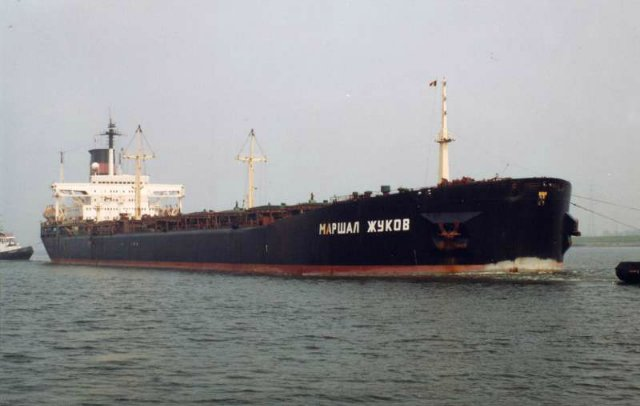
\includegraphics[scale=0.5]{Figs/marshl_jukov.jpg}
    \caption{Судно <<Маршал Жуков>>}
    \label{fig:jukov}
\end{figure}

И подобные явления, как оказалось, описывались и задолго до Франклина. В своей <<естественной истории>> Плиний Старший говорит о похожем явлении \cite{Plinii}. Позднее <<мертвая вода>> была воспроизведена в лабораторных условиях исследователями из франции \cite{deadWater}. Запись эксперимента доступна на видеохостинге youtube \cite{deadWaterVideo}.


Математически описать возникновение внутренних волн можно записав уравнение для сил, которые действуют на выведенную из равновесия частицу жидкости(Рис. \ref{fig:Forces}):

\begin{equation}
    m_b \vec{a}_b = \vec{P} + \vec{G}
\end{equation}
где $\vec{P}=\rho_w \vec{g} S \cdot h$ это сила Архимеда, $\rho_w$ плотность жидкости того слоя на котором находится частица, $\vec{g}$ -- ускорение свободного падения, $S$ -- площадь стороны частицы, $h$  -- глубина. $\vec{G} = \rho_b \vec{g} S \cdot h$,  $\rho_b$ -- плотность частицы жидкости.

В проекции на вертикальную ось:

\begin{equation}
    \frac{d^2 \xi}{dt^2} = \frac{(\rho_w-\rho_b)}{\rho_b}\cdot g
\end{equation}

Тут $\xi$ будет обозначать отклонение от положения равновесия $z_0$, тогда очевидно что плотность воды вокруг частицы и плотность частицы будет равна в положении равновесия при $\xi=0$ $\rho_w(z_0)=\rho_b$ тогда уравнение можно переписать:

\begin{equation}
    \frac{d^2 \xi}{dt^2} = \frac{\rho_w(z_0+\xi)-\rho_b}{\rho_b}\cdot g
    \label{eq:beg}
\end{equation}

Введем переобозначение, $z=z_0+\xi$ тогда правая часть уравнения запишется $$\frac{\rho_w(z_0+\xi)-\rho_b}{\rho_b}\cdot g = \frac{\rho_w(z)-\rho_w(z_0)}{\rho_w(z_0)}\cdot g = \frac{1}{\rho(z_0)} \frac{\rho_w(z)-\rho_w(z_0)}{z-z_0}\cdot(z-z_0) g$$

При достаточно малом $t$ отклонении от положения равновесия $z$ будет также мало, что дает нам возможность перейти к производной по $z$, а $\rho_w$ переобозначим как $\rho$ и окончательно запишем:

\begin{equation}
    \frac{d^2 \xi}{dt^2} =\frac{1}{\rho} \frac{d\rho}{z}\xi \cdot g
\end{equation}

Решение этого дифференциального уравнения ищется в виде периодической функции, это значит, что частица совершает колебания около своего положения равновесия:

\begin{equation}
    \xi(t)=A cos(\omega t + \phi)
\end{equation}

подставим выражения $\xi(t)$ в уравнение:

\begin{equation}
    \ddot{\xi} = - A \omega^2 cos(\omega t + \phi )
\end{equation}

или если выразить правую часть через $\xi$

\begin{equation}
    \ddot{\xi} = - \omega^2  \xi
    \label{eq:final}
\end{equation}

Подставим (\ref{eq:final}) в (\ref{eq:beg}):

\begin{equation}
    -\omega^2 \xi = \frac{1}{\rho_0}\cdot \frac{d \rho}{d z} \xi g
\end{equation}

Выразим частоту колебаний частицы:

\begin{equation}
    \omega(z) = N(z) = \sqrt{- \frac{g}{\rho_0}\cdot\frac{d \rho(z)}{dz}}
\end{equation}

Эта частота называется частота плавучести или Частота Брента — Вяйсяля. В океане она составляет величину порядка $10^{-3}$ $\frac{1}{\textup{с}}$ \cite{King2012}.

\begin{figure}
    \centering
    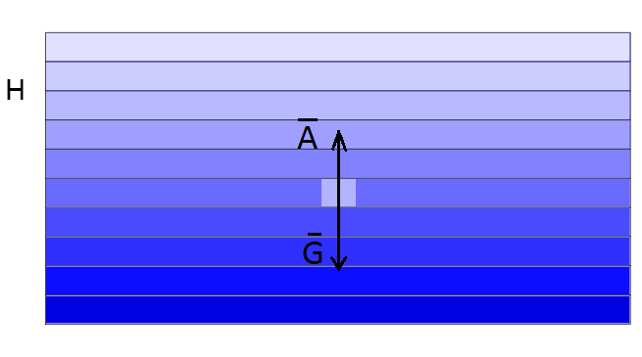
\includegraphics[scale=0.8]{Figs/Forces.png}
    \caption{Схематичное представление сил действующие на частицу выведенную из равновесия в стратифицированной жидкости, цветом показана плотность.}
    \label{fig:Forces}
\end{figure}

\begin{figure}
    \centering
    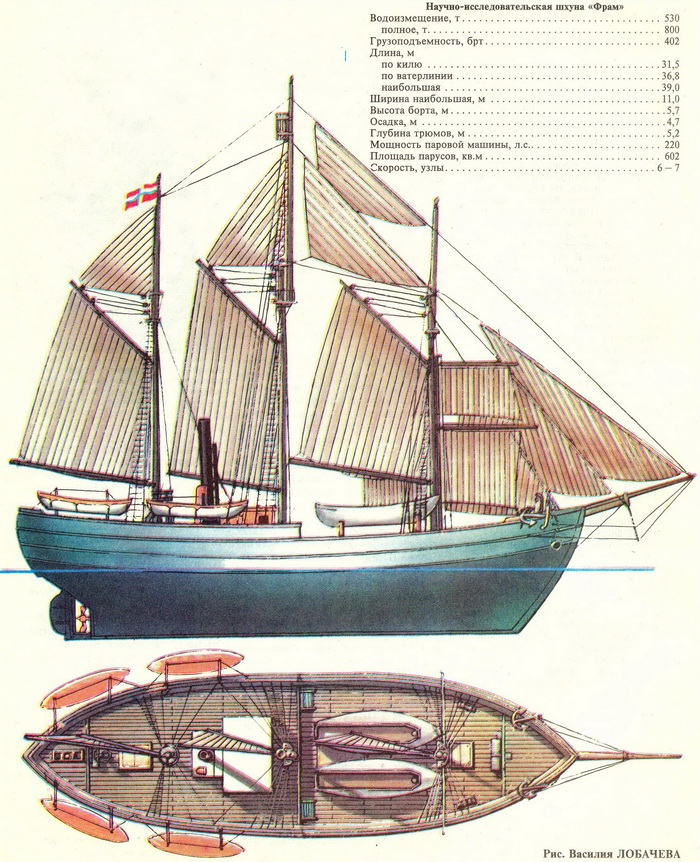
\includegraphics[width=1\textwidth]{Figs/FRAM.jpg}
    \caption{Исследовательское судно <<Фрам>>}
    \label{fig:fram}
\end{figure}

\begin{figure}
    \centering
    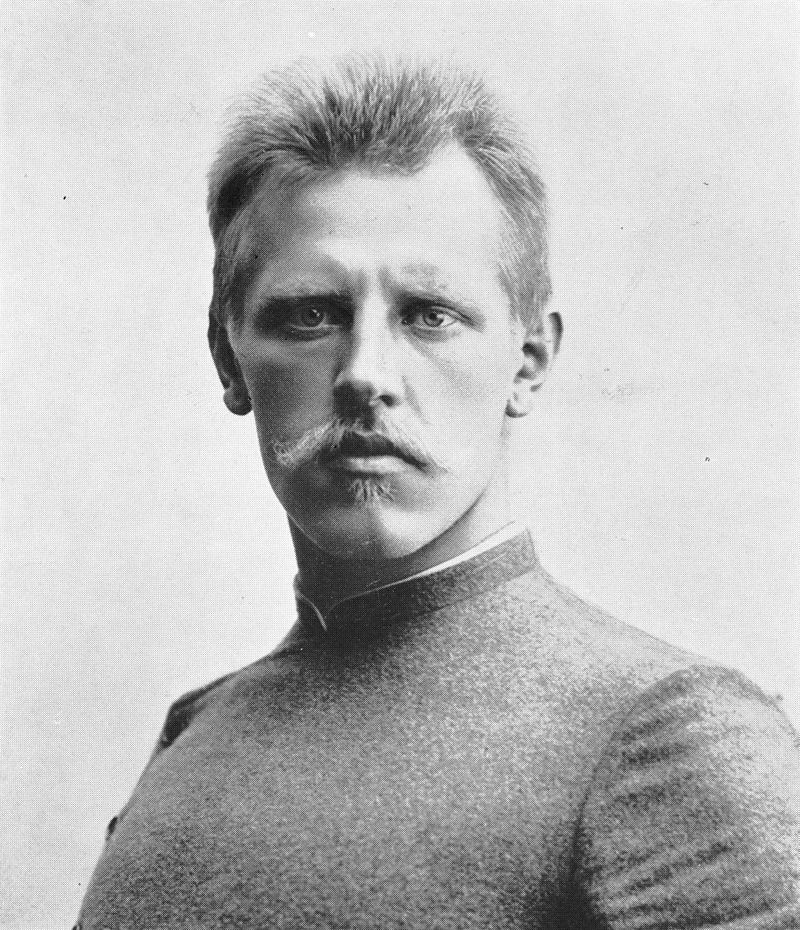
\includegraphics[scale=2.5]{Figs/800px-Fridtjof_Nansen.jpg}
    \caption{Фритьоф Ведель-Ярлсберг Нансен (1861-1930)}
    \label{fig:Nansen}
\end{figure}

\section{Обзор литературы}

Внутренние волны очень распространенное явление в океане. Существуют они благодаря перепадам плотности на разной глубине, сила плавучести играет роль восстанавливающей силы. Океаны являются одним из естественных примеров стратифицированных сред. Основные источники внутренних волн в океане это приливные эффекты, которые сопряжены с движением Земли относительно Солнца и Луны относительно Земли.

Внутренние волны активно взаимодействуют с другими океаническими структурами \cite{Rainville2006} и с неровностями океанического дна \cite{DAUXOIS1999}. Процессы перемещения внутренних волн их взаимодействия друг с другом и океаническими структурами различных масштабов образуют собой явление называемое энергетическим каскадом\cite{Garrett1972}. Энергетический каскад способствует поддержанию глобальной океанической циркуляции и перемешиванию\cite{Nikurashin2012,Munk1998}. Тем не менее, механизмы вносящие крупномасштабный приливный вклад в движение внутренних волн недостаточно понятны \cite{Ivey2008,Polzin1997} и каскадный процесс остается одной из фундаментальных проблем современной океанографии. Главным образом остаются вопросы связи крупномасштабных и мелкомасштабных явлений.

Одним из объяснений этой связи могут послужить аттракторы внутренних гравитационных волн. Это явление, при котором внутренние волны многократно отражаясь от поверхности океана, его дна и неровностей движутся по замкнутым орбитам. Возникновение такого явление возможно лишь в том случае, когда на дне океана имеются определенные комбинации геометрических неровностей. Аттракторы передают кинетическую энергию крупномасштабных эффектов, такие как приливы и внутренние волны большой длинны к мелкомасштабным явлениям волновой турбулентности и перемешиванию. Происходит это благодаря явлению фокусировки, в результате которого длинна внутренних волн уменьшается, но увеличивается амплитуда.

Возможность возникновения аттракторов в океане с реальной геометрией дна уже исследовалась\cite{Tang2010}. Например, топология северной части хребта Лусона имеет соответствующую геометрию. Эксперименты~\cite{ECHEVERRI2011} подтверждают возможность образования аттракторов внутренних волн. Кроме того при моделировании внутренних волн в условиях случайного разреза геометрии океанического дна, был сделан вывод, что с немалой вероятностью возможны возникновения аттракторов по одному на каждую сотню километров океанического дна \cite{Guo2015}. Тем не менее стоит отметить, что на данный момент нет свидетельств наблюдаемых волновых аттракторов. Возможно это связано с тем, что теоретические работы\cite{Guo2015} относятся к двумерному океану, но также существуют трехмерные конфигурации геометрий в которых возможны существования трехмерных волновых аттракторов\cite{Drijfhout2007,Manders2004}. Кроме того, в теоретическом представлении аттракторов внутренних волн не учитывается шероховатость поверхностей отражения. Однако надежность теоретических соображений о возможности существования трехмерных аттракторов была экспериментально проверена\cite{Hazewinkel2010}. Кроме того волновые явления в океане часто имеют целый спектр частот\cite{Garrett1972}, в то время как многочисленные эксперименты проводятся лишь с монохроматическим источником внутренних волн.

Предполагается, что аттракторы могут влиять не только на перемешивание, но и на движение мелких животных, явление седиментации и эрозию прибрежных конструкций.

Работы по фокусировке внутренних волн и образованию устойчивых аттракторов ведутся с конца двадцатого века. Первое теоретическое предсказание аттракторов было сделано Лео Маасом в 1995 году\cite{Maas1995}. Через два года последовали экспериментальные исследования этого явления, теоретические результаты были воспроизведены\cite{Maas1997}. Эффекты фокусировки характерны не только для стратифицированной жидкости, но и для вращающихся \cite{articleMaas2003,Veronis1970}. В дальнейшем теоретические основы явления были пересмотрены на основании данных эксперимента\cite{Lam2008}.

Вместе с развитием вычислительной техники развивались и инструменты численного моделирования физических явлений. Во втором десятилетии двадцать первого века стало возможным численное моделирование трехмерных аттракторов внутренних волн. Первая удачная попытка была предпринята с использованием метода спектральных элементов\cite{Brouzet2016,Brouzet_2016}. При сравнении с экспериментом ошибка численного моделирования составила не больше 10\%. Также была предпринята попытка моделирования аттрактора внутренних волн с помощью метода конечного объема\cite{Brouzet2014}. Количественно воспроизвести результаты, полученные с помощью метода спектральных элементов не удалось.
Традиционно для моделирования аттракторов применяются уравнения Навье-Стокса в приближении Буссинеска. Однако существует ряд работ, где вместо классического подхода используется квазигидродинамический\cite{ElizarBook}. Квазигидродинамические уравнения позволяют добиться большей точности\cite{Kraposhin20182} при моделировании методом конечного объема.

Результаты работы представляют собой интерес для приложений в океанологии, экологии, биологии, астрофизики и вращающихся технических систем. 

\paragraph{Цель работы} -- изучение явления бигармонического аттрактора, которое возникает при воздействии на стратифицированную жидкость двухчастотным волнопродуктором.  
С этой целбю были посталены следующие задачи \textbf{задачи}:

\begin{itemize}

  \item Нахождение интервала частот внешних воздействий, при которых возникает аттрактор внутренних волн.
  
  % Изучение интервалов частот внешних воздействий и других параметров, при которых происходит аккумуляция волновой энергии, в частности волновых аттракторов.

%    \item Нахождение частотных параметров приводящих к образованию аттракторов в резервуаре.
    
  % \item Обзор существующих методов моделирования аттракторов внутренних волн. Выявление их достоинств и недостатков.
    
  \item Реализация численных экспериментов с помощью двух подходов: спектрально-элементного и конечно-объемного.

  \item Разработка новой программы для моделирования аттракторов внутренних волн на основе квазигидродинамического подхода.
    
  \item Верификация результатов численного моделирования.

  \item Описание особенностей волновых режимов при бигармоническом воздействии и значительно отличающихся частотах воздействия и малых амплитудах.

  \item Описание особенностей волновых режимов при бигармоническом воздействии, близких частотах воздействия и малых амплитудах.
    
  \item Описание особенностей нелинейных волновых режимов при бигармоническом воздействии и близких частотах воздействия.

  \item Сравнение динамики средней кинетической энергии и пульсации кинетической энергии для монохроматического режима и различных бигармонических режимов.
    

    
\end{itemize}

\paragraph{Методы решения поставленных задач}

Для решения поставленых задач были использованы методы математического моделирования механики сплшных сред, такие как метод спектральных элементов и метд конечного объема. Для предсказания формы аттрактора внутренних волн использовался метод трассировки лучей. Для анализа данных использовался метод построения частотно-временных диаграмм при помощи быстрого преобразования Фурье.

\paragraph{Научная новизна работы} выражается в конкретных реузьтатах:
\begin{enumerate}[1.]
  \item Получены аналитические выражения для границ частотного интервала существования аттракторов внутренних волн.% конфигурации (1,1). 
    
  \item Получена геометрия течения, которая возникает в трапециевидном резервуаре, наполненном стратифицированной жидкостью при воздействии на жидкость внешними возмущениями с двумя различными частотами. 
    
  \item Проведён анализ результатов моделирования аттрактора внутренних волн при бигармоническом воздействии, полученных с помощью метода спектральных элементов. Для различных комбинаций возмущающих частот построен спектр, частотно-временная диаграмма и зависимость средней кинетической энергии от времени. 
    
  \item Реализован квазигидродинамический подход на базе метода конечного элемента. Проведено сопоставление результатов моделирования методов конечных объемов и методом спектральных элементов.
\end{enumerate}

\paragraph{Достоверность результатов}

Достоверность полученных результатов гарантируется строгой математической постановкой, верификацией и валидацией разработанного алгоритма для решения поставленной задачи.

% \paragraph{Объектом исследования} являются волновые режимы возникающие %в естественных условиях 
% при двух источниках внешних воздействий на стратифицированную жидкость в трапециевидном резервуаре.

% %Приложения включают в себя задачи океанологии, астрофизики и технических вращающихся систем при периодических воздействиях. 

% %\paragraph{В исследовании использованы следующие методы:}
% \begin{itemize}
%   \item [    В исследовании использованы \textbf{
% методы:}]
%   \item методы численного моделирования конечного объема;
%   \item метод спектральных элементов;
%   \item метод трассировки лучей;
%   \item Фурье анализ полученных результатов, в том числе по скользящему окну;
%   \item разложение по эмпирическим модам;
% \end{itemize}

% % В работе рассматриваются резервуары в форме трапеций различных конфигураций, заполненных стратифицированной жидкостью. Одна из стенок резервуара представляет собой волнопродуктор, который порождает внутренние волны в стратифицированной среде. Результаты разработки предоставляют возможность проводить моделирование аттракторов внутренних волн в условиях сложной геометрии и неортогональных сетках. 



\paragraph{Практическая значимость} 

Ранее эксперименты по исследованию бигармонических аттракторов, как численные так и натурные, не проводились. Теоретически, бигармонический аттрактор представляет собой новую устойчивую структуру, которая образуется в стратифицированной жидкости при воздействии на нее периодическим двухчастотным возмущением.

Положения и выводы диссертационного исследования могут быть использованы для подбора параметров  волнового аттрактора в лабораторных условиях или при численном моделировании. Среди возможных приложений результатов работы — задачи моделирования аттракторов внутренних волн на сложных геометриях, задачи моделирования течений со сложным спектром частотных воздействий на стратифицированную жидкость. Работа является первым шагом к моделированию течений, возникающих в условиях, приближенных к реальным океаническим, что позволит выяснить форму и вид природных аттракторов внутренних волн. Комбинация методов конечного объёма и квазигидродинамических уравнений позволила добиться существенного улучшения в точности моделирования и дала инструмент к  усложнению геометрии расчётной области. Разработанная программа может быть применена не только к задачам моделирования аттрактора, но и к другим задачам гидродинамики с дозвуковыми и трансзвуковыми скоростями.

\paragraph{На защиту выносятся следующие положения:}
\begin{itemize}

  \item Найдены аналитические выражения для границ диапазонов частот колебаний волнопродуктора, которые способны порождать аттракторы.

  \item Показано, что при значительном отличии частот внешних воздействий и малых амплитудах воздействий волновой режим представляет из себя совокупность независимо существующих волновых аттракторов.

  \item Показано, что при близких частотах внешних воздействий и малых амплитудах возникает режим с биениями, характерной особенностью которых является малая амплитуда пульсаций на убывающем склоне огибающей.

  \item Показано, что при близких частотах внешних воздействий и средних амплитудах возникают биения, на одном цикле которых успевает происходит переход к турбулентности через триадные резонансы, и реламинаризация.
    
  \item Обнаружено наличие фазового сдвига между биениями на волнопродукторе и биениями средней кинетической энергии во всем объеме.
    
%   \item 
%     Сравнение динамики средней кинетической энергии и пульсации кинетической энергии для монохроматического режима и различных бигармонических режимов указывает на то, что на убывающем склоне огибающей большая доля кинетической энергии переходит в бегущие волны по сравнению с возрастающей фазой.

  \item Разработана и верифицирована новая программа для моделирования аттракторов внутренних волн и в целом динамики стратифицированных сред.
    
%  \item Реализация численных экспериментов с помощью двух подходов: спектрально-элементного и конечно-объемного.

%  \item Проведена верификация результатов численного моделирования.
%    Проведение численных экспериментов различными методами.
    
%  \item Количественный анализ результатов численных экспериментов. 
    
%  \item Верификация разработанной программы.
    
\end{itemize}

\paragraph{Личный вклад автора}

Исследования, результаты которых выносятся на защиту, были получены лично соискателем. Соискатель аналитически нашел диапазон частот внешнего воздействия при которых образуется аттрактор внутренних волн. Соискатель подобрал параметры эксперемента, провел расчеты и проанализировал полученные данные. Также принимал непосредственное участие в разработке реализации квазигидродинамического подхода на базе открытого программного комлекса OpenFOAM. Научный руководитель И. Н. Сибгатуллин поставил первоначальную задачу и участввал в обсуждении результатов. 

\paragraph{Аппробация работы}

Материалы диссертации представлялись на различных конференциях, семинарах, как российсих так и международных:


\begin{itemize}
  \item Открытая международная конференция ИСП РАН им. В.П.Иванникова. 5-6 декабря 2019 г, г. Москва Главное здание Российской академии наук (устный доклад).
  \item Международная конференция «Суперкомпьютерные технологии математического моделирования» (СКТеММ’19), 19-21 июня 2019, г. Москва (устный доклад).
  \item 13th OpenFOAM Workshop, Shanghai, China, Китай, 24-29 июня 2018 (устный доклад).
  \item XXIII международная конференция «Нелинейные задачи теории гидродинамической устойчивости и турбулентность». 25 февраля - 4 марта 2018, Московская область, г. Звенигород (стендовый доклад).
  \item Рязанов Д.А. Открытая конференция ИСП РАН им. В.П. Иванникова. 30 ноября - 1 декабря 2017 г. Москва главное здание Российской академии наук (стендовый доклад).
\end{itemize}

\paragraph{Публикации}

По результатам диссертации опубликовано 12 научныйх работ, входящих в базы данных и системы цитирования РИНЦ, Scopus, Web of Science, 2 из них входят в Перечень рецензируемых научных изданий, рекомендованных Высшей раттестационной комиссией. Зарегестрирована программа для ЭВМ.

\paragraph{Сутрктура и объем диссертации}

% В ходе работ был разработан программный продукт, который подлежал государственной регистрации № 2018663951.

%
\mainmatter % это включает нумерацию глав и секций в документе ниже
%
\chapter{Обзор литературы}

Внутренние волны очень распространенное явление в океане\cite{holton_encyclopedia_2003}. Существуют они благодаря перепадам плотности на разной глубине, сила плавучести играет роль восстанавливающей силы \cite{Eckart1961}. Океаны являются одним из естественных примеров стратифицированных сред. Основные источники внутренних волн в океане это приливные эффекты, которые сопряжены с движением Земли относительно Солнца и Луны относительно Земли \cite{Egbert2000}.

\section{История развития интереса к явлению внутренних волн и текущее состояние}

Считается установленным, что впервые внутренние волны наблюдал американский ученый Франклин в восемнадцатом веке с помощью простой экспериментальной установки. Она представляла собой емкость, заполненную несмешивающимися жидкостями различной полости~\cite{Sudolski}. Однако в конце восемнадцатого века вблизи полуострова Таймыр произошло событие, которое заострило внимание научного сообщества на этом интересном явлении. В то время в этом районе пролегал маршрут исследовательского судна <<Фрам>>(Рис. \ref{fig:fram}) под руководством Фритьофа Нансена (Рис. \ref{fig:Nansen}).

\begin{figure}
    \centering
    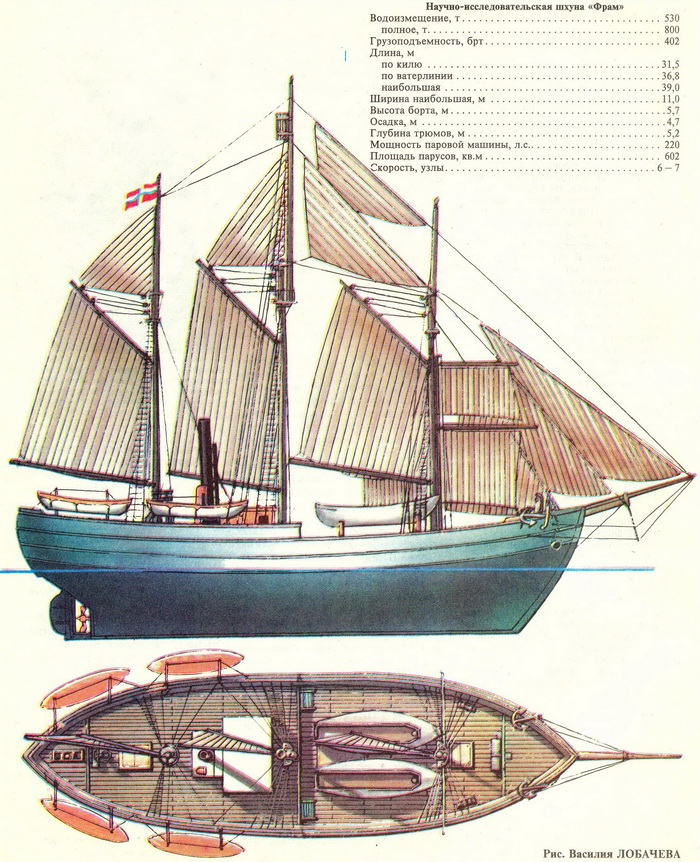
\includegraphics[width=1\textwidth]{Figs/FRAM.jpg}
    \caption{Исследовательское судно <<Фрам>>}
    \label{fig:fram}
\end{figure}

\begin{figure}
    \centering
    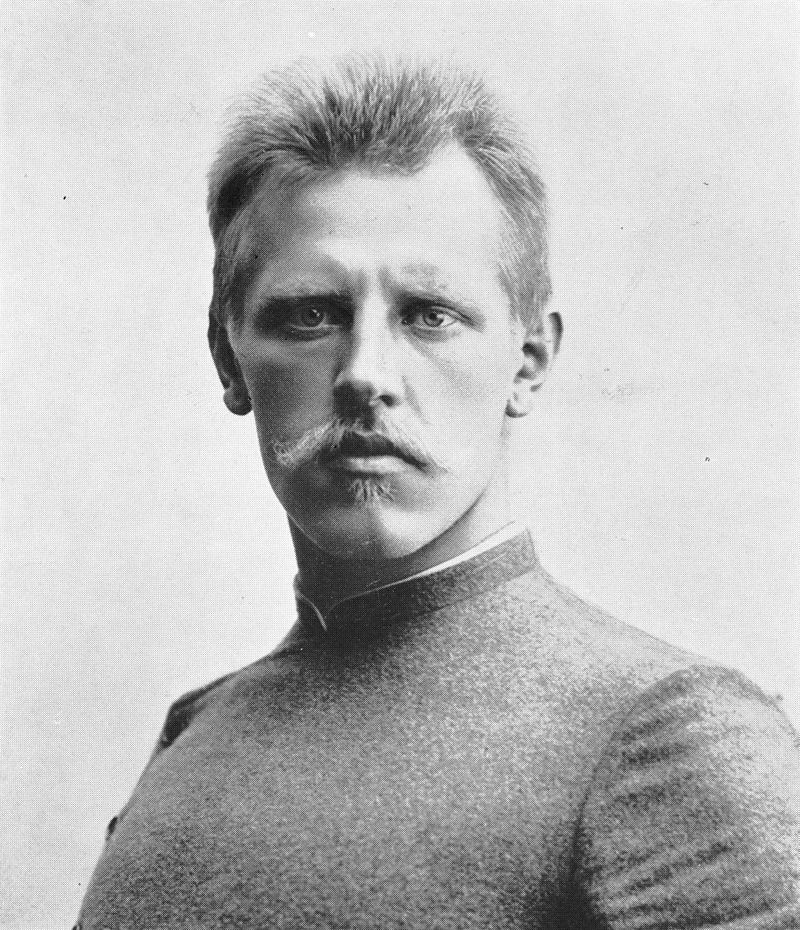
\includegraphics[scale=2.5]{Figs/800px-Fridtjof_Nansen.jpg}
    \caption{Фритьоф Ведель-Ярлсберг Нансен (1861-1930)}
    \label{fig:Nansen}
\end{figure}

Однажды во время штиля судно остановилось. Скорость его движения резко снизилась.  «Чтобы пройти то небольшое расстояние, которое мы и на веслах прошли бы в полчаса или того меньше, «Фраму» понадобилась целая вахта», -- как писал сам Нансен. При этом исследователь отмечал, что вода на поверхности была пресной, потому как натекла с оттаявших ледников. А на глубине сравнимой с осадкой судна, резко становилась соленой. Позднее его записи послужили стимулом для теоретических исследований этого явления. В итоге было установлено, что почти вся энергия судового двигателя сдвигает не судно, а образует волны на поверхности раздела между слоями пресной и соленой воды. Это явление получило название <<мертвая вода>>.

Также существует еще одно свидетельство этого явления. Теплоход «Маршал Жуков» при проходе пролива Дарданеллы угодил в <<мертвую воду>> летом 1981 года. Уже в сентябре в отраслевой газете <<черноморец>> капитан-наставник Александр Косилов подробно описал как в течение четырех суток судно, держащее курс из Канады в Новороссийск, боролось с феноменом. Согласно комментариям руководителя аналитико-исследовательской группы управления инвестиций и проектов ОАО «Новошип», кандидата технических наук, профессора кафедры судовождения ГМУ им. адмирала Ф.Ф. Ушакова Юрия Пескова современные суда в значительной степени подвержены влиянию подобных явлений\cite{MorVest}. На то есть причины:

\begin{itemize}
    \item Экономия топлива вынуждает снижать скоростные режимы
    \item Борьба за уменьшение углекислых выбросов предписывает снижать мощность двигателя
\end{itemize}


\begin{figure}
    \centering
    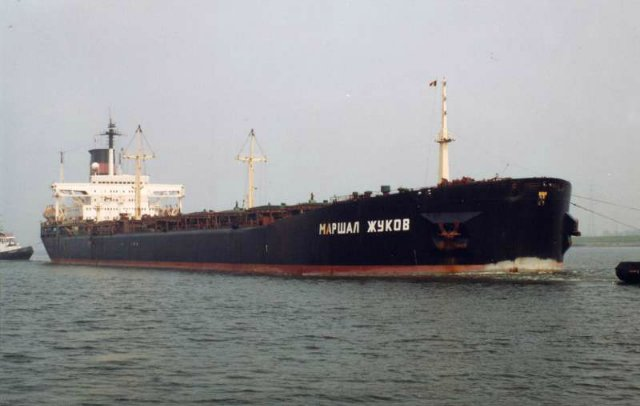
\includegraphics[scale=0.5]{Figs/marshl_jukov.jpg}
    \caption{Судно <<Маршал Жуков>>}
    \label{fig:jukov}
\end{figure}

И подобные явления, как оказалось, описывались и задолго до Франклина. В своей <<естественной истории>> Плиний Старший говорит о похожем явлении \cite{Plinii}. Позднее <<мертвая вода>> была воспроизведена в лабораторных условиях исследователями из франции \cite{deadWater}. Запись эксперимента доступна на видеохостинге youtube \cite{deadWaterVideo}.

О возможности внутренних волн многократно фокусироваться после отражения от наклонных поверхностей стало известно сравнительно недавно \cite{Gardner1989}. Благодаря этому в стратифицированной жидкости могут образовываться аттракторы внутренних волн -- замкнутые траектории по которым циркулируют внутренние волны \cite{Maas1995}.

Внутренние волны активно взаимодействуют с другими океаническими явлениями \cite{Rainville2006} и с неровностями океанического дна \cite{DAUXOIS1999}. Процессы перемещения внутренних волн их взаимодействия друг с другом и океаническими структурами различных масштабов образуют собой явление называемое энергетическим каскадом \cite{Garrett1972}. Энергетический каскад способствует поддержанию глобальной океанической циркуляции и перемешиванию \cite{Nikurashin2012,Munk1998}. Тем не менее, механизмы вносящие крупномасштабный приливный вклад в движение внутренних волн недостаточно понятны \cite{Ivey2008,Polzin1997} и каскадный процесс остается одной из фундаментальных проблем современной океанографии. Главным образом остаются вопросы связи крупномасштабных и мелкомасштабных явлений.

Одним из объяснений этой связи могут послужить аттракторы внутренних гравитационных волн. Это явление, при котором внутренние волны многократно отражаясь от поверхности океана, его дна и неровностей движутся по замкнутым орбитам. Возникновение такого явления возможно лишь в том случае, когда на дне океана имеются определенные комбинации геометрических неровностей. Аттракторы передают кинетическую энергию крупномасштабных эффектов, такие как приливы и внутренние волны большой длинны к мелкомасштабным явлениям волновой турбулентности и перемешиванию. Происходит это благодаря явлению фокусировки, в результате которого длинна внутренних волн уменьшается, но увеличивается амплитуда.

Возможность возникновения аттракторов в океане с реальной геометрией дна уже исследовалась\cite{Tang2010}. Например, топология северной части хребта Лусона имеет соответствующую геометрию. Эксперименты~\cite{ECHEVERRI2011} подтверждают возможность образования аттракторов внутренних волн. Кроме того при моделировании внутренних волн в условиях случайного разреза геометрии океанического дна, был сделан вывод, что с немалой вероятностью возможны возникновения аттракторов по одному на каждую сотню километров океанического дна \cite{Guo2015}. Тем не менее стоит отметить, что на данный момент нет свидетельств наблюдаемых волновых аттракторов. Возможно это связано с тем, что теоретические работы \cite{Guo2015} относятся к двумерному океану, но также существуют трехмерные конфигурации геометрий в которых возможны существования трехмерных волновых аттракторов \cite{Drijfhout2007,Manders2004}. Кроме того, в теоретическом представлении аттракторов внутренних волн не учитывается шероховатость поверхностей отражения. Однако надежность теоретических соображений о возможности существования трехмерных аттракторов была экспериментально проверена \cite{Hazewinkel2010}. Кроме того волновые явления в океане часто имеют целый спектр частот \cite{Garrett1972}, в то время как многочисленные эксперименты проводятся лишь с монохроматическим источником внутренних волн.

Предполагается, что аттракторы могут влиять не только на перемешивание, но и на движение мелких животных, явление седиментации и эрозию прибрежных конструкций.

Работы по фокусировке внутренних волн и образованию устойчивых аттракторов ведутся с конца двадцатого века. Первое теоретическое предсказание аттракторов было сделано Лео Маасом в 1995 году\cite{Maas1995}. Через два года последовали экспериментальные исследования этого явления, теоретические результаты были воспроизведены\cite{Maas1997}. Эффекты фокусировки характерны не только для стратифицированной жидкости, но и для вращающихся \cite{articleMaas2003,Veronis1970}. В дальнейшем теоретические основы явления были пересмотрены на основании данных эксперимента\cite{Lam2008}.

Вместе с развитием вычислительной техники развивались и инструменты численного моделирования физических явлений. Во втором десятилетии двадцать первого века стало возможным численное моделирование трехмерных аттракторов внутренних волн. Первая удачная попытка была предпринята с использованием метода спектральных элементов \cite{Brouzet2016,Brouzet_2016}. При сравнении с экспериментом ошибка численного моделирования составила не более 10\%. Помимо этого аттракторы внутренних волн моделировались с помощью метода конечного объема \cite{Brouzet2014}. Количественно воспроизвести результаты, полученные с помощью метода спектральных элементов не удалось.
Традиционно для моделирования аттракторов применяются уравнения Навье-Стокса в приближении Буссинеска. Однако существует ряд работ, где вместо классического подхода используется квазигидродинамический \cite{ElizarBook}. Квазигидродинамические уравнения позволяют добиться большей точности \cite{Kraposhin20182} при моделировании методом конечного объема.



\section{Общая теория внутренних гравитационных волн}

\subsection{Стратификация}

\begin{figure}
    \centering
    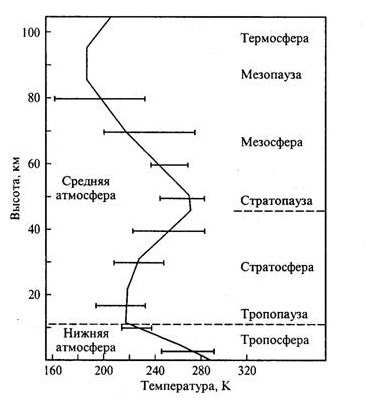
\includegraphics{pics/tempDistrib.jpg}
    \caption{Распределение температуры в атмосфере по высоте}
    \label{fig:temperatureDistrib}
\end{figure}

Рисунок \ref{fig:temperatureDistrib} из \cite{geoThermins} показывает типичное распределение температуры воздуха по высоте. Стратификация в атмосфере измеряется с помощью метеозондов. Выделяются различные регионы с примерно постоянным градиентом температуры: тропосферу, стратосферу, мезосферу и термосферу \cite{saha2008the}. Границы между этими зонами называют тропопауза, стратопауза и мезопауза. Температурный профиль не монотонен, но плотность атмосферы зависит от температуры и давления, которые значительно меняются с высотой. Например, от земли (Высота $= 0$ км.) до стратопаузы (Высота $= 50$ км.), давление уменьшается на три порядка и на шесть до верхних слоев атмосферы (Высота $= 100$ км.). Для этого вводится понятие потенциальной температуры, которая измеряется при одинаковом давлении \cite{gidrometDict}.  Частота плавучести в атмосфере составляет порядка $10^{-2}$ 1/с. 

Океан стратифицирован по солености, как это показано на рис \ref{fig:salVSdepth}. Стратификация зависит от географического положения. Однако можно выделить три основных типа слоев:

\begin{itemize}
    \item Смешанный слой, расположенный несколько ниже поверхности. Этот слой имеет толщину около $100$ м и однороден по температуре и солености. Перемешивание происходит из-за различных взаимодействий с атмосферой. 
    
    \item Область ниже смешанного слоя. В этой области плотность изменяется квазилинейно с глубиной на несколько километров. Частота плавучести в этом слое обычно составляет $10^{-4}$ --- $10^{-3}$ рад/с.
    
    \item Пикноклин, где плотность резко меняется. Этот слой очень тонкий и расположен между смешанным слоем и глубинной областью. Таким образом, он демонстрирует сильные градиенты плотности, а частота плавучести в этом слое обычно составляет $10^{-2}$ рад/с. Пикноклин ограничивает обмены между смешанным слоем и глубинной областью из-за сильных градиентов плотности.
\end{itemize}


\begin{figure}
    \centering
    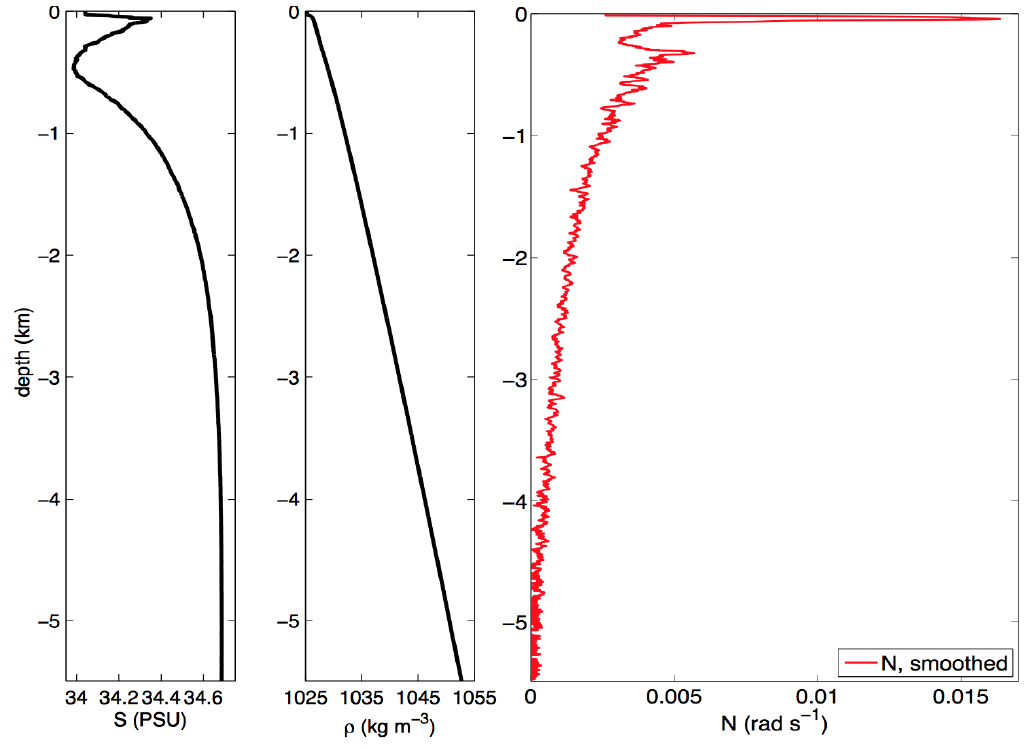
\includegraphics[scale = 0.6]{pics/salinityAndNVsDepth.png}
    \caption{Распределение солености, плотности и частоты плавучести в океане по глубине}
    \label{fig:salVSdepth}
\end{figure}

\subsection{Генерация внутренних волн}

В атмосфере внутренние волны рождаются от взаимодействия ветров и рельефа земной поверхности.

В океане есть два механизма ответственных за происхождение внутренних волн:

\begin{itemize}
    \item Излучение внутренних волн топографией морского дна во время приливных течений. К примеру обтекание приливным потоком топологической возвышенности высотой 100 м при частоте плавучести $10^{-3}$ рад/приведет к возникновению внутренних волн если скорость потока превышает $0.4$ м/с. Рисунок \ref{fig:intWaveGen} из \cite{GarrettSc} показывает как приливное воздействие генерирует внутренние волны. Также от взаимодействия с шельфом, как показано в левой части рисунка \ref{fig:intWaveGen}
    \item Из-за взаимодействия с атмосферой посредством ветра. 
\end{itemize}

\begin{figure}
    \centering
    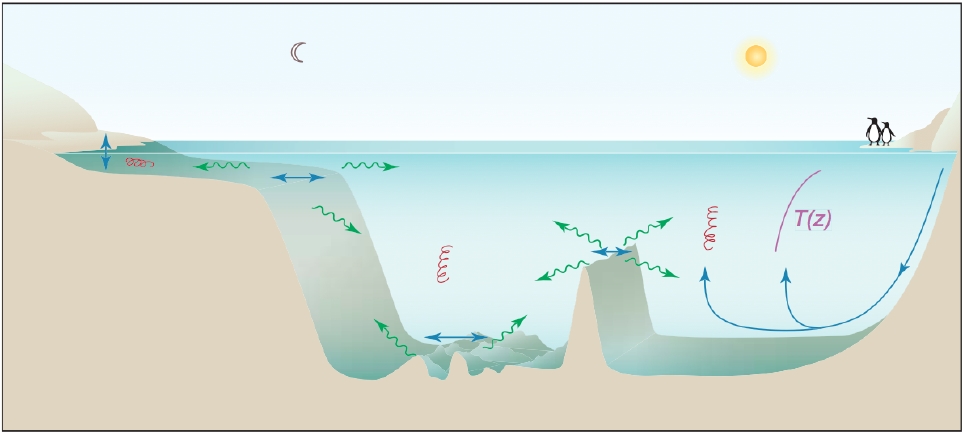
\includegraphics[scale=0.6]{pics/IntGen.png}
    \caption{Генерация внутренних волн за счет приливного воздействия \cite{GarrettSc}. В центре волны вызваны приливами. Слева волны вызваны приливами вблизи континентального шельфа. Волны способствуют возникновению турбулентности, и перемешиванию в океане, влияют на профиль плотности, как показано справа.}
    \label{fig:intWaveGen}
\end{figure}

Внутренние волны могут вызывать перемешивание в океане и играть существенную роль в океанографической циркуляции. Вертикальное перемешивание в стратифицированной жидкости имеет первостепенное значение для глобального обращения. В около 90\% из примерно 60 ТВт мощности, поступающей от ветра в океан, рассеивается в пределах 100 м от поверхности воды \cite{Ferrari2009} за счет волновой турбулентности \cite{nazarenko2011wave, Yarom2014} и опрокидывания внутренних волн \cite{Perlin2013}. Механизм перемешивания при больших глубинах менее изученное явление. Океанографические данные говорят о том, что для поддержания имеющийся стратификации необходимо 1 ТВт мощности \cite{Munk1998}. Постоянное воздействие приливных эффектов на океан имеет мощность порядка 11 ТВт \cite{Garrett2007}. Поэтому должен существовать механизм конвертации (так называемый энергетический каскад) мощности поступающей со стороны приливных эффектов в многообразие внутренних волн различных масштабов и перемешиванию \cite{Munk1998}.

Причем нет единой точки зрения на то какие механизмы перемешивания в глубинных слоях океана являются доминирующими \cite{Ivey2008}. Существуют описания составляющих энергетического каскада, фокусировка внутренних волн \cite{BHLER2007}, отражение внутренних волн \cite{dauxois_young_1999}, преломление волн в слоях с резким перепадом плотности \cite{mathur_peacock_2009}, интерференция волн и их взаимодействие со сложной топографией морского дна \cite{ECHEVERRI2011}, внутренние волны Ли \cite{MacKinnon2013,Nikurashin2013}. Допускаются сценарии с триадной резонансной неустойчивостью \cite{Bourget2013}, гидростатической неустойчивостью \cite{mathur_peacock_2009}, сдвиговой неустойчивостью и неустойчивостью нижнего слоя на склонах \cite{Gayen2010, Lamb2014}.

Математически описать возникновение внутренних волн можно записав уравнение для сил, которые действуют на выведенную из равновесия частицу жидкости(Рис. \ref{fig:Forces}):

\begin{figure}
    \centering
    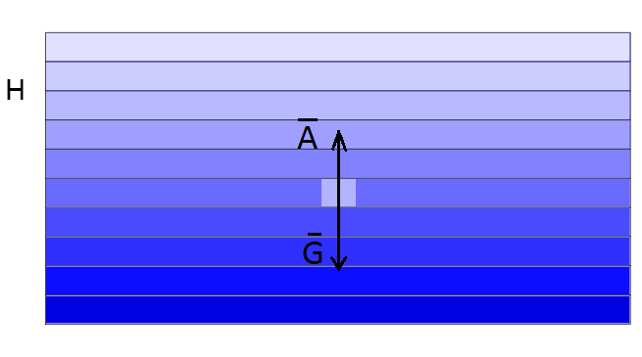
\includegraphics[scale=0.8]{Figs/Forces.png}
    \caption{Схематичное представление сил действующие на частицу выведенную из равновесия в стратифицированной жидкости, цветом показана плотность.}
    \label{fig:Forces}
\end{figure}

\begin{equation}
    m_b \vec{a}_b = \vec{P} + \vec{G}
\end{equation}
где $\vec{P}=\rho_w \vec{g} S \cdot h$ это сила Архимеда, $\rho_w$ плотность жидкости того слоя на котором находится частица, $\vec{g}$ -- ускорение свободного падения, $S$ -- площадь стороны частицы, $h$  -- глубина. $\vec{G} = \rho_b \vec{g} S \cdot h$,  $\rho_b$ -- плотность частицы жидкости.

В проекции на вертикальную ось:

\begin{equation}
    \frac{d^2 \xi}{dt^2} = \frac{(\rho_w-\rho_b)}{\rho_b}\cdot g
\end{equation}

Тут $\xi$ будет обозначать отклонение от положения равновесия $z_0$, тогда очевидно что плотность воды вокруг частицы и плотность частицы будет равна в положении равновесия при $\xi=0$ $\rho_w(z_0)=\rho_b$ тогда уравнение можно переписать:

\begin{equation}
    \frac{d^2 \xi}{dt^2} = \frac{\rho_w(z_0+\xi)-\rho_b}{\rho_b}\cdot g
    \label{eq:beg}
\end{equation}

Введем переобозначение, $z=z_0+\xi$ тогда правая часть уравнения запишется $$\frac{\rho_w(z_0+\xi)-\rho_b}{\rho_b}\cdot g = \frac{\rho_w(z)-\rho_w(z_0)}{\rho_w(z_0)}\cdot g = \frac{1}{\rho(z_0)} \frac{\rho_w(z)-\rho_w(z_0)}{z-z_0}\cdot(z-z_0) g$$

При достаточно малом $t$ отклонении от положения равновесия $z$ будет также мало, что дает нам возможность перейти к производной по $z$, а $\rho_w$ переобозначим как $\rho$ и окончательно запишем:

\begin{equation}
    \frac{d^2 \xi}{dt^2} =\frac{1}{\rho} \frac{d\rho}{z}\xi \cdot g
\end{equation}

Решение этого дифференциального уравнения ищется в виде периодической функции, это значит, что частица совершает колебания около своего положения равновесия:

\begin{equation}
    \xi(t)=A cos(\omega t + \phi)
\end{equation}

подставим выражения $\xi(t)$ в уравнение:

\begin{equation}
    \ddot{\xi} = - A \omega^2 cos(\omega t + \phi )
\end{equation}

или если выразить правую часть через $\xi$

\begin{equation}
    \ddot{\xi} = - \omega^2  \xi
    \label{eq:final}
\end{equation}

Подставим (\ref{eq:final}) в (\ref{eq:beg}):

\begin{equation}
    -\omega^2 \xi = \frac{1}{\rho_0}\cdot \frac{d \rho}{d z} \xi g
\end{equation}

Выразим частоту колебаний частицы:

\begin{equation}
    \omega(z) = N(z) = \sqrt{- \frac{g}{\rho_0}\cdot\frac{d \rho(z)}{dz}}
\end{equation}

Эта частота называется частота плавучести или Частота Брента — Вяйсяля. В океане она составляет величину порядка $10^{-3}$ $\frac{1}{\textup{с}}$ \cite{King2012}.


\subsection{Математические модели для изучения внутренних гравитационных волн}

Для описания движения несжимаемой жидкости используется уравнение Навье-Стокста. Но при небольшом перепаде плотности допустимо использовать уравнение Навье-Стокса в приближении Буссинеска, которое учитывает сжимаемость в члене с плавучестью.

\begin{equation}
 \large \frac{\partial \vec U}{\partial t} + (\vec U \cdot \nabla) \vec U = - \frac{1}{\rho_m} \nabla \hat p + \nu \Delta \vec U  + \vec f,
 \label{eq:momClassic}
\end{equation}
Уравнение переноса соли $s$:
\begin{equation}
 \large \frac{\partial \rho_s}{\partial t} + \vec U \cdot \nabla \rho_s  = \nabla \cdot \frac{\nu}{Sc} \left ( \nabla \rho_s \right ),
 \label{eq:transClassic}
\end{equation}
\begin{equation}
 \large \nabla \cdot \vec U  = 0.
 \label{eq:contClassic}
\end{equation}

Здесь $\vec{U}$ -- вектор скорости с компонентами $u_x,u_y; \nu$ -- кинематическая вязкость жидкости; $\rho_m$ -- значение плотности на верхней границе; $\rho_s$ -- добавка к плотности обусловленная наличием солености; приведенное давление $\hat{p}=p-p_0$, разница между полным и гидростатическим давлением; $\vec{f}=\frac{\rho_s}{\rho_m} \vec{g}$ -- восстанавливающая сила; Число Шмидта представляет собой отношение кинематической вязкости и коэффициента диффузии:  $Sc = \frac{\nu}{D}$. 

В данной работе помимо классических уравнений Навье-Стокса в приближении Буссинеска используются квазигидродинамические уравнения, работа над которыми ведется в институте прикладной математики имени Келдыша с восьмидесятых годов двадцатого века \cite{bookELIZ}. Различие между уравнениями Навье-Стокса несжимаемой жидкости и квазигидродинамическими уравнениями заключается в дополнительных диссипативных слагаемых. Эти слагаемые были первоначально введены для разреженного газа как способ сохранить инвариантность при пространственно-временном усреднении\cite{AIAAJ1995}. Физическая интерпретируемость в случае несжимаемой жидкости после обобщения теряется, но математически уравнения все еще верны \cite{Elizarova2011}. Как будет показано ниже диссипативные слагаемые могут быть весьма полезны при численном моделировании. 

\subsection{Линеаризованная теория внутренних гравитационных волн}

Ранее рассмотрена полная система уравнений, описывающая движение стратифицированной жидкости. Чтобы упростить задачу, можно предположить, что поток является двумерным и содержится в плоскости $xOz$ без изменений в направлении $y$. В этих рамках, используя уравнение неразрывности (\ref{eq:contClassic}), можно ввести функцию тока, определяемую как

\begin{equation}
    \frac{\partial \psi}{\partial x} = - u_z \;\;\;\;\;\;\;\; и \;\;\;\;\;\;\;\; \frac{\partial \psi}{\partial z} = - u_x
\end{equation}

тогда можно переписать уравнения (\ref{eq:momClassic}), (\ref{eq:transClassic}) и (\ref{eq:contClassic}) как

\begin{equation}
    \partial_{tz} \psi + J(\partial_z \psi, \psi) = - \frac{1}{\rho} \partial_x P + \nu \partial_z \Delta \psi,
    \label{eq:tokz}
\end{equation}

\begin{equation}
    \partial_{tx} \psi + J(\partial_x \psi, \psi) = \frac{\rho_s}{\rho_m}\vec{g}+\frac{1}{\rho}\partial_z P + \nu \partial_x \Delta \psi,
    \label{eq:tokx}
\end{equation}

\begin{equation}
    \partial_t \rho_s + J(\rho_s,\psi) = \nabla \cdot \frac{\nu}{Sc} (\nabla \rho_s) + \frac{d \rho}{dz} \partial_x \psi,
\end{equation}
где $J$ это яклбиан определенный как $J(f,g) = \partial_x f \partial_z g - \partial_z f \partial_x g.$ Обозначим как $\partial_j \psi =\frac{\partial \psi}{\partial j}$, где $j$ обозначает $x,y$ или $t$. 

В дальнейшем предполагается, что возмущения плотности $\rho_s(x; z; t)$ малы по сравнению с фоновой стратификацией $\rho(z)$. Это предположение полностью верно как в океане, так и экспериментах, рассматриваемых тут. Таким образом, возмущения плотности ограничиваются менее чем 10\% средней стратификации. 

Дифференцируя уравнение (\ref{eq:tokz}) по $z$, а (\ref{eq:tokx}) по $x$ и складывая их получаем

\begin{equation}
    \partial_t(\Delta \psi) + J (\Delta \psi, \psi) - \nu \Delta (\Delta \psi) = \frac{g}{\rho_m} \partial_x \rho_s,
    \label{eq:tokzz}
\end{equation}

\begin{equation}
    \partial_t \rho_s + J(\rho_s,\psi) - \nabla \cdot \frac{\nu}{Sc} (\nabla \rho_s) = -N^2 \frac{\rho_m}{g}\partial_x \psi.
    \label{eq:tokxx}
\end{equation}

Уравнения (\ref{eq:tokzz}) и (\ref{eq:tokxx}) описывают нелинейную динамику вязкой стратифицированной жидкости с диффузией. Уравнения для линейной динамики получаются путем пренебрежения нелинейными членами. Это приводит к

\begin{equation}
    \partial_t(\Delta \psi) + \nu \Delta (\Delta \psi) = \frac{g}{\rho_m} \partial_x \rho_s,
\end{equation}

\begin{equation}
    \partial_t \rho_s - \nabla \cdot \frac{\nu}{Sc} (\nabla \rho_s) = -N^2 \frac{\rho_m}{g}\partial_x \psi.
\end{equation}

Рассмотрим решение в виде плоской волны к линеаризованной системе: $\psi = \psi_0 exp(i\omega t - i \vec{k} \cdot \vec{r})$ и $\rho_s=\rho_m exp(i\omega t - i \vec{k}\cdot \vec{r})$. Волновой вектор $\vec{k}=k_x \vec{e}_x + k_z \vec{e}_z$ и его модуль $k$.

Линейная система может быть записана в матричном виде

\begin{equation}
    \left(\begin{array}{cc} -k^2(i\omega + \nu k^2) & i \frac{g}{\rho_m}k_x
    \\[15pt] iN^2 \frac{\rho_m}{g}kx & i\omega + \frac{\nu}{Sc} k^2 \end{array}\right)
    \left(\begin{array}{c}\psi \\[15pt] \rho_s\end{array}\right) = 
    \left(\begin{array}{c}0 \\[15pt] 0\end{array}\right).
\end{equation}

Можно найти нетривиальное решение этой системы

\begin{equation}
    k^2 \left( i\omega + \nu k^2 \right) \left(i \omega \frac{\nu}{Sc} k^2 \right) + N^2 k^2_x = 0.
\end{equation}

Если рассмотреть систему без диссипативных членов, убрать диффузию и теплопроводность то уравнение примет вид:

\begin{equation}
    \left(\frac{\omega}{N}\right)=\frac{k^2_x}{k^2} \;\;\;\;\;\;\;\; или \;\;\;\;\;\;\;\; \frac{\omega}{N}=\pm \frac{|k_x|}{k}.
\end{equation}

Это дисперсионное соотношение линейных внутренних волн в невязкой и недиффузионной жидкости. Его можно записать, используя угол $\theta$ между вертикальной осью $z$ и волновым вектором $\vec{k}$

\begin{equation}
    \frac{\omega}{N} = \pm sin \theta.
    \label{eq:dispersion}
\end{equation}

Это чисто геометрическое соотношение, которое показывает как распространяются волны в стратифицированной жидкости(Рис. \ref{fig:ermExp}). Угол распространения определяется только частотой плавучести и частотой вынужденных колебаний. Наконец, стоит отметить, что в дисперсионном соотношении отсутствует характерный масштаб длины. Таким образом, длина внутренних волн определяется граничными условиями, только источником волн.

\begin{figure}
    \centering
    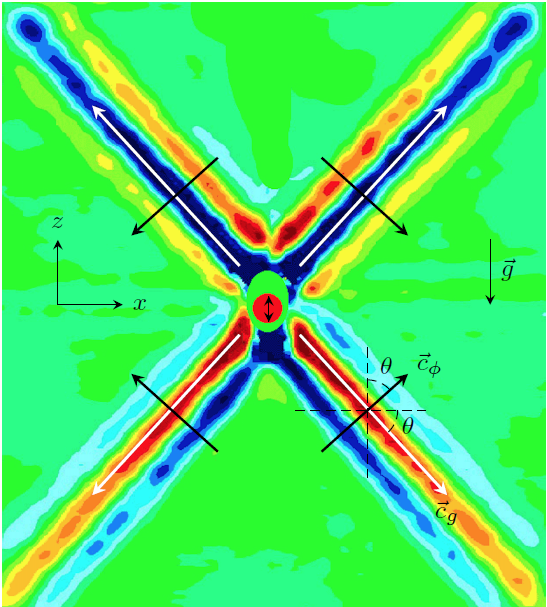
\includegraphics[scale=0.5]{Figs/Experement_Erm.png}
    \caption{Внутренние волны, излучаемые вертикально колеблющимся цилиндром, распространяются в линейно стратифицированной жидкости и  показаны красным в центре рисунка. Векторы групповой скорости показаны белым цветом, а векторы фазовой скорости — черным. Цветами обозначены поля горизонтального градиента плотности, полученные экспериментально Евгением Ерманюком с использованием методики SyS. Рисунок из \cite{brouzet:tel-01361201}}
    \label{fig:ermExp}
\end{figure}

%\subsection{Численные методы исследования волновых течений в неоднородных средах}

\section{Аттракторы внутренних волн}

Первые работы по аттракторам внутренних волн были проведены Лео Маасом, сначала теоретические \cite{Maas1995}, а потом и экспериментальные \cite{brouzet1997laboratory}.  

Дисперсионное соотношение дает мощный инструмент позволяющий качественно предсказать траекторию движения пучков внутренних волн, не только по удалению от источника, но и при отражении от препятствий (Рис. \ref{fig:internalReflection}). Поле отражения внутренняя волна сохраняет угол с вертикалью. Кроме того внутренние волны обладают свойством фокусировки, что выражается в сокращении расстояния между двумя параллельно пущенными лучами поле отражения от наклонной стенки. 

\begin{figure}
    \centering
    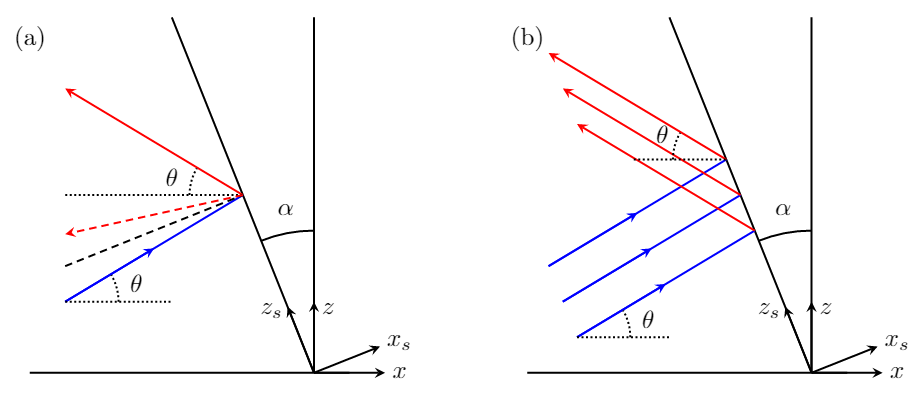
\includegraphics[scale=0.5]{Figs/angle_of_reflection.png}
    \caption{Отражение пучка внутренних волн от наклонной стенки. а) Отражение одного пучка, падающий волновой луч изображен синим цветом, отраженный от наклонной стенки красным, точками обозначена биссектриса. Черным пунктиром обозначен перпендикуляр к наклонной поверхности, красным пунктиром луч отраженный <<зеркально>> по правилу Евклида. b) Отражение нескольких волновых лучшей от наклонной поверхности, отраженные лучи стали ближе, чем были падающие.}
    \label{fig:internalReflection}
\end{figure}

Многократное отражение от стенок трапециевидного резервуара приведет к постепенному сближению лучей, которые, в конечном итоге замкнуться на траектории в форме параллелепипеда (Рис. \ref{fig:RayTr}). 

\begin{figure}
    \centering
    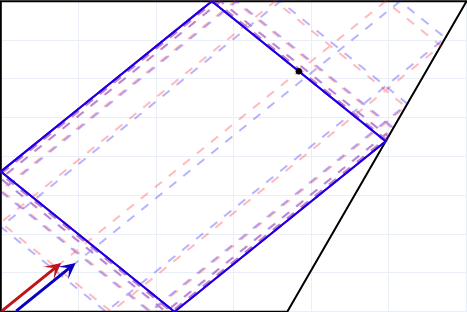
\includegraphics[scale=0.8]{Figs/RayTracing.png}
    \caption{Результат многократного отражения двух параллельных лучей внутренних волн}
    \label{fig:RayTr}
\end{figure}



\subsection*{Заключение к главе 1}

Явление внутренних волн широко распространенное в океане оказывает огромное влияние на природные процессы происходящих в его недрах, на климатические процессы в атмосфере, а также на жизнедеятельность человека. 

В этой главе рассматривается история открытия и развития теории внутренних волн, переломным моментом в исследовании явлений связанных с динамикой стратифицированной жидкости можно считать экспедицию Нансена. Проведен обзор литературы по теме внутренних гравитационных волн, благодаря специальному закону отражения от наклонных поверхностей, который определяется дисперсионным соотношением у внутренних волн имеется свойство фокусировки. Фокусировка позволяет внутренним волнам образовывать аттракторы внутренних волн в закрытых акваториях. В главе рассмотрены геометрические и физические принципы фокусировки. 
\chapter{Методы исследования аттракторов внутренних волн}

Качественно, аттракторы внутренних волн, возникающие после многократной фокусировки в акватории, выражаются в повышенной интенсивности движения стратифицированной жидкости около геометрического контура фокусировки. Первичный способ изучить форму аттрактора -- это метод трассировки лучей \cite{Maas1997}. Этот метод помогает при в поиске аттракторов в акваториях с различными геометрическими характеристиками \cite{Guo2015}. Метод трассировки лучей дает ответ на вопрос о принципиальном существовании аттрактора в конкретной геометрии. Однако, Этот метод не дает данных о поле скорости вблизи аттрактора и не учитывает вязкость жидкости, в которой это явление может возникать.

Получение количественных характеристик аттрактора внутренних волн невозможно без использования экспериментальных установок или численного моделирования \cite{Brouzet2016}. Экспериментальными исследованиями аттракторов внутренних волн впервые начал заниматься Лео Маас с 1997 года \cite{Maas1997}. В 2011 году была построена установка в Массачусетском технологическом университете и проведены серии экспериментов \cite{Hazewinkel2011} после сотрудничества с Лео Маасом \cite{Hazewinkel2010}. Сейчас экспериментальным исследованием аттракторов занимаются Терри Доксуа \cite{Dauxoisetal2018} во Франции, а в России -- Евгений Ерманюк \cite{brouzet1997laboratory}.

Наиболее точным методом численного моделирования аттракторов внутренних волн является метод спектральных элементов \cite{NEK5000}. Разница с экспериментом составила всего 10\% \cite{Brouzet2014}. Однако, у него имеются свои недостатки о которых упоминается в этой главе. Альтернативой методу спектральных элементов служит метод конечных элементов \cite{ferziger2002computational} и широко используемые в рамках этого метода алгоритм PISO \cite{Issa1986-PISO}. Алгоритм PISO также не лишен недостатков о которых будет сказано позднее. Еще одной альтернативой является квазигидродинамический подход и регуляризированные уравнения \cite{ElizarBook}. Предполагается, что такой подход при сохранении удобства использования и модификации методов будет обладать повышенной точностью. 

\section{Исследование свойств волновых течений с помощью трассировки лучей}

В предыдущей главе уже была затронута тема трассировки лучей. Это геометрическое представление пучков внутренних волн в виде лучей \cite{Maas1995}, которые отражаются от поверхностей согласно дисперсионному соотношению (\ref{eq:dispersion}).

Прослеживая траекторию лучей в замкнутом трапециевидном резервуаре можно определить будет ли при данных геометрических параметрах и частоте волнопродуктора образовываться аттрактор внутренних волн. Каждое отражение от наклонной стенки увеличивает амплитуду фазовой скорости внутренней волны, но уменьшает ее длину. На существование и форму аттрактора влияют несколько факторов:

\begin{itemize}
    \item Угол наклона фокусирующей поверхности ($\alpha$)
    \item Частота плавучести $N$
    \item Частота колебаний волнопродуктора $\omega$
    \item Длинна резервуара $L_1$
    \item Высота резервуара $H$
\end{itemize}

Для простоты рассмотрим трапециевидный резервуар 

\begin{figure}[!ht]
    \centering
    \begin{tikzpicture}[scale=1, z={(-.707,-.5)}]
    \draw (3.6,0,0) -- (0,0,0) -- (0,4,0)--(6,4,0)--(3.6,0,0);
    %\draw (3.6,0,0) -- (3.6,0,-1) -- (6,4,-1) -- (6,4,0) -- cycle;
    %\draw (6,4,0) -- (0,4,0) -- (0,4,-1) -- (6,4,-1);
    \draw (-0.5,2,0) node{};
    \draw (4.1,-.2,-1.5) node{};
    \draw (3.5,5,0) node{};
    \draw[<->] (-0.1,0) --node[above,rotate=90] {$H$} (-0.1,4);
    \draw[<->] (0,4.1,0) --node[above,] {$L_1$} (6,4.1,0);
    \draw[<->] (0,-0.1,0) --node[below,] {$L_2$} (3.6,-0.1,0);
    \draw [black, thick] (5.5,4) arc [start angle=180, end angle=240, radius=0.5cm]
        node [left] {$\alpha$};
    \draw[thick,->] (5.5,1,0) -- (6.5,1,0) node[anchor=north east]{$x$};
    \draw[thick,->] (5.5,1,0) -- (5.5,2,0) node[anchor=north west]{$z$};
    \draw[thick,->] (0,0,0) -- (3,2,0) ;

    \draw [black, thick] (0.42,0.31) arc [start angle=30, end angle=90, radius=0.5cm] node [above right] {$\theta$};
    
    \end{tikzpicture}
    \caption{Область фокусировки лучей внутренних волн, где $\theta = sin \frac{\omega}{N}$}
    \label{fig:domainup}
\end{figure}

Задачу трассировки лучей можно упростить, введя параметры. В своей работе он предлагает параметризовать резервуар фокусировки внутренних волн следующим образом(Рис. \ref{fig:domainTran}):

Применяется преобразование горизонтальной координаты, которое перемещает систему координат таким образом, чтобы левый конец резервуара соответствовал координате $-1$, а правый $1$. Вводится параметр $d$ который обозначает расстояние от нуля новой горизонтальной оси до точки соприкосновения наклонной стенки с горизонтальной осью.
\begin{equation}
    x'=\frac{x\cdot 2}{L_1}-1
    \label{eq:transformX}
\end{equation}

Затем преобразование вертикальной координаты, которое сжимает или растягивает высоту резервуара так, чтобы угол отражения и распространения внутренних волн стал $45^\circ$. При этом вводится параметр $\tau$, который обозначает новую высоту резервуара. 
\begin{equation}
    z'=\frac{z\cdot 2}{L_1}\sqrt{\frac{N^2}{\omega^2}-1}
    \label{eq:transformZ}
\end{equation}

Таким образом вместо пяти определяющих параметров для геометрической задачи, остаются всего два, $d$ и $\tau$.

Благодаря методу трассировки лучей можно геометрически предсказать форму аттрактора внутренних волн. 

\begin{figure}
    \begin{subfigure}{\textwidth}
    \centering
    \begin{tikzpicture}[scale=0.7]
        \draw[thick] (0,0)--(0,4)node[left]{$H$}--(6,4)--(3.7,0)--(0,0);
        \draw[dashed] (6,4) -- (6,0)node[below]{$L_1$};
        \draw[thick,->] (6.2,2)->node[above]{$x'=\frac{x\cdot 2}{L_1}-1$}(14,2);
        \draw[->] (0,0)->(0,5)node[above]{$z$};
        \draw[->] (0,0)->(7.5,0)node[right]{$x$};
        \draw[->] (0,0)->(1.2,1);
        \draw[black] (0.5,0) arc [start angle=0, end angle=75, radius=0.25cm] node [right] {$\theta$};
        \draw[thick] (14.2,0)node[below]{$-1$}--(14.2,4)node[left]{$H$}--(20.2,4)--(17.9,0)node[below]{$d$}--(14.2,0);
        \draw[dashed] (20.2,4) -- (20.2,0)node[below]{$1$};
        \draw[->] (17.2,0)->(21.7,0)node[right]{$x'$};
        \draw[->] (17.2,0)->(17.2,5)node[above]{$z$};
        \draw[->] (14.2,0)->(15.4,1);
        \draw [black] (14.7,0) arc [start angle=0, end angle=75, radius=0.25cm] node [right] {$\theta$};
    \end{tikzpicture}
    \caption{Горизонтальное преобразование расчетной области}
    \end{subfigure}
    
    \begin{subfigure}{\textwidth}
    \centering
    \begin{tikzpicture}[scale=0.7]
        \draw[thick] (0,0)--(0,4)node[left]{$H$}--(6,4)--(3.7,0)--(0,0);
        \draw[dashed] (6,4) -- (6,0)node[below]{$L_1$};
        \draw[thick,->] (6.2,2)->node[above]{$z'=\frac{z\cdot 2}{L_1}\sqrt{\frac{N^2}{\omega^2}-1}$}(14,2);
        \draw[->] (0,0)->(0,5)node[above]{$z$};
        \draw[->] (0,0)->(7.5,0)node[right]{$x$};
        \draw[thick] (14.2,0)--(14.2,4.8)node[left]{$\tau$}--(20.2,4.8)--(17.9,0)--(14.2,0);
        \draw[black] (0.5,0) arc [start angle=0, end angle=75, radius=0.25cm] node [right] {$\theta$};
        \draw [black] (14.7,0) arc [start angle=0, end angle=80, radius=0.25cm] node [right] {$45^\circ$};
        \draw[->] (0,0)->(1.2,1);
        \draw[->] (14.2,0)->(15.4,1.2);
        \draw[dashed] (20.2,4.8) -- (20.2,0)node[below]{$L_1$};
        \draw[->] (17.2,0)->(21.7,0)node[right]{$x$};
        \draw[->] (14.2,0)->(14.2,6)node[above]{$z'$};
    \end{tikzpicture}
    \caption{Вертикальное преобразование расчетной области}
    \end{subfigure}
    \caption{Преобразования расчетной области для процедуры получения диаграммы Мааса}
    \label{fig:domainTran}
\end{figure}

На рисунке \ref{fig:RayTr923x1455} изображен резервуар до перехода и после перехода к параметрам $(d,\tau)$.

\begin{figure}
    \begin{subfigure}[с]{0.45\textwidth}
        \centering
        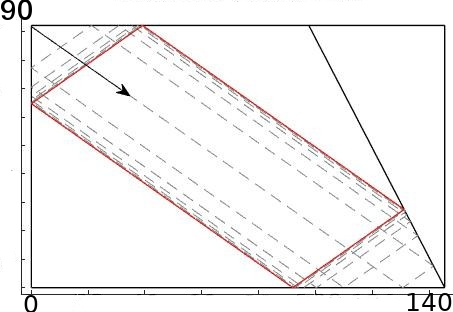
\includegraphics[scale=0.45]{Figs/RayTr923x1455.jpeg}
        \caption{Трассировка лучей,\\ $H=92.3$, $L=145.5$, $\theta = 35.13^{\circ}$,\\ $\alpha = 27.4^{\circ}$}
    \end{subfigure}
    \begin{subfigure}[r]{0.45\textwidth}
        \centering
        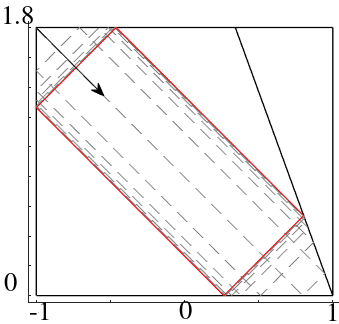
\includegraphics[scale=0.45]{Figs/RTdtau.png}
        \caption{Трассировка лучей в преобразованной геометрии, \\ $\tau = 1.8$, $d = 0.34$}
    \end{subfigure}
    
    \caption{Результат работы процедуры трассировки лучей и результат перехода к параметрам $(d,\tau)$}

    \label{fig:RayTr923x1455}
\end{figure}

После преобразования можно перейти в плоскость параметров и отобразить цветом среднюю кинетическую энергию в резервуаре \cite{Maas1997} и области формирования аттрактора внутренних волн. Средняя кинетическая энергия в резервуаре получена прямым численным моделированием (Рис. \ref{fig:diagramm}). 

\begin{figure}
    \centering
    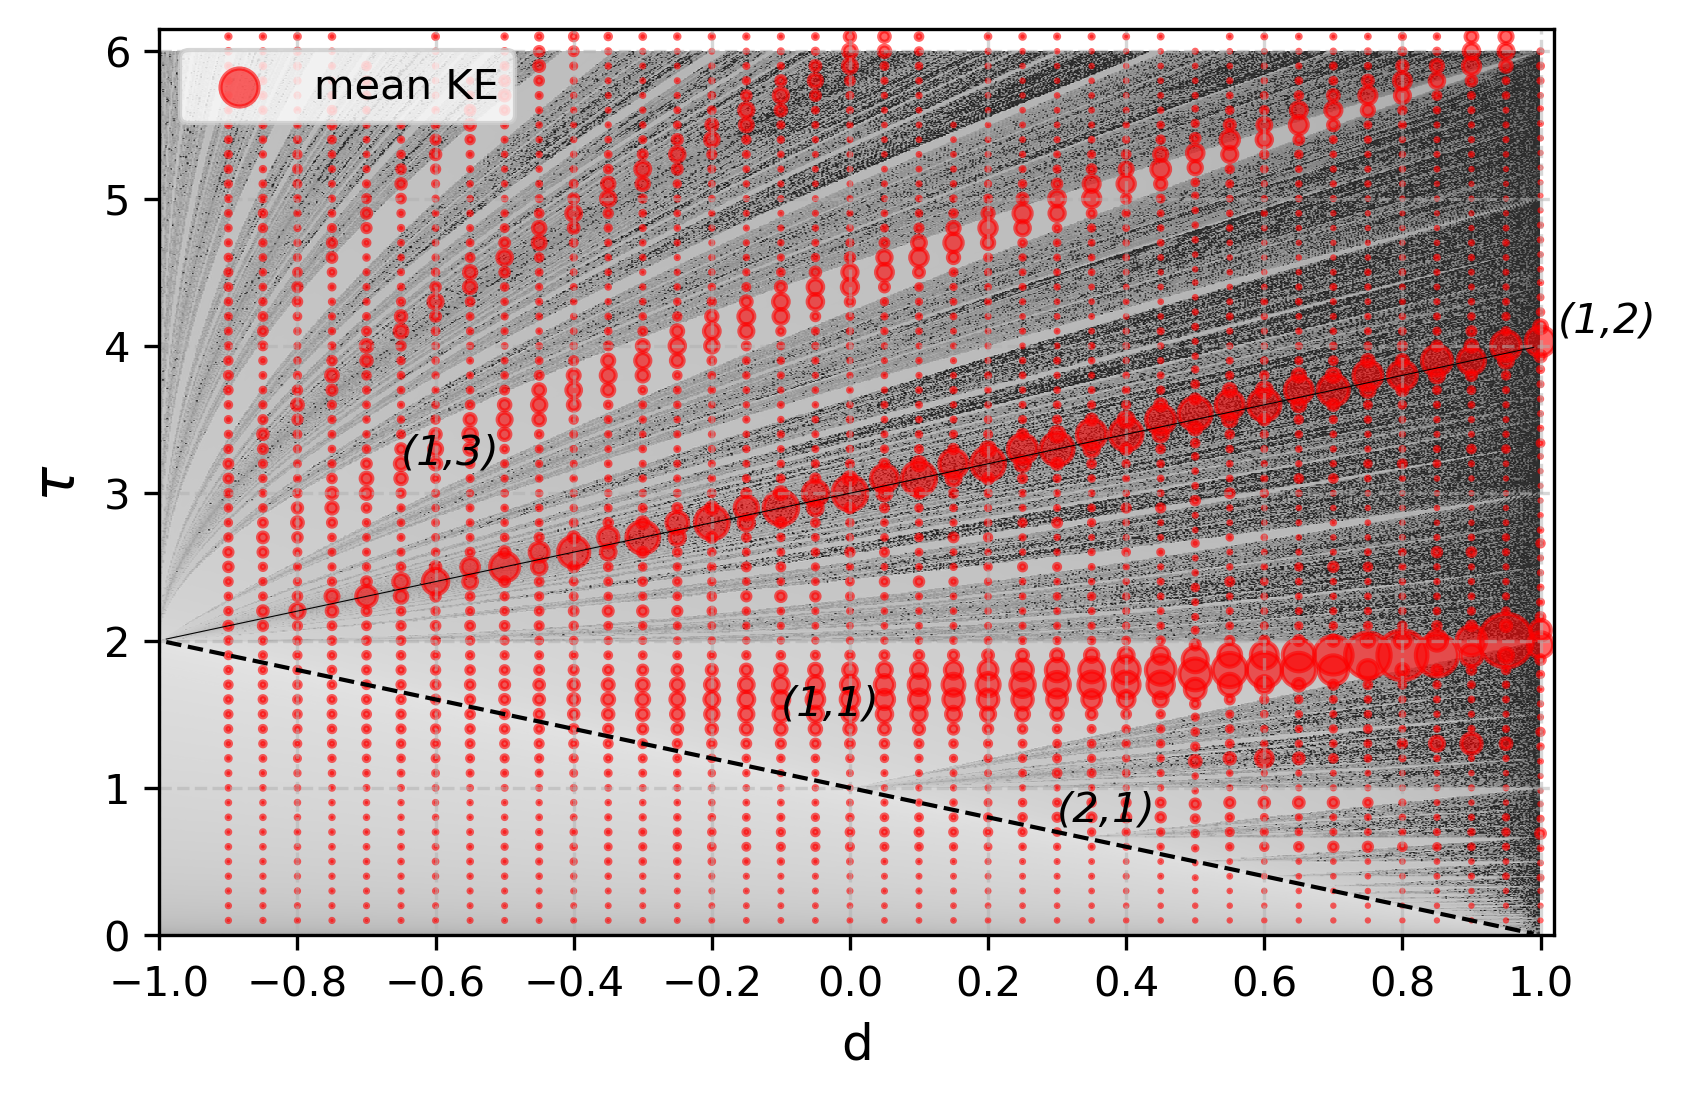
\includegraphics{pics/KEandLyap.png}
    \caption{Средняя кинетическая энергия во множестве резервуаров, в координатах ($\tau$,$d$). Величина точки показывает относительное количество кинетической энергии в резервуаре. Светлые области -- области существования аттрактора. }
    \label{fig:diagramm}
\end{figure}

\subsection{Критические частоты и диапазон существования аттракторов внутренних волн}

В этой работе рассматривается зона существования аттракторов помеченная на рисунке \ref{fig:diagramm} маркером $(1,1)$. Влиять на параметр $d$ можно изменяя геометрические характеристики резервуара. А параметр $\tau$ регулируется изменением частоты колебаний волнопродуктора. Если изменяется параметр $\tau$, или просто $\omega$, то изменяется и форма аттрактора внутренних волн. Аналитически можно получить диапазон частот в зависимости от геометрических параметров резервуара, который определит существование аттрактора или его отсутствие при данных параметрах.

Найдем такие параметры системы, чтобы аттрактор вырождался в отрезки для этого положим $\tau=2$. Выбор такого значения обусловлен углом распространения внутренних волн $\theta = 45^{\circ}$. Это значит, что волна пущенная из левого верхнего угла упрется в правый нижний угол так как длинна резервуара $=2$ от $-1$ до $1$(см рис. \ref{fig:trivAttr}). Если в уравнение (\ref{eq:transformZ}) подставить вместо $z$ высоту резервуара $H$, то получим:

\begin{equation}
    \tau=\frac{2H}{L} \sqrt{\frac{N^2}{\omega^2}-1}.
\end{equation}

Теперь подставим $\tau=2$:

\begin{equation}
    1=\frac{H}{L} \sqrt{\frac{N^2}{\omega^2}-1}.
\end{equation}

Выразим отсюда $\omega$:

\begin{equation}
    \omega=\frac{NH}{\sqrt{L^2+H^2}}.
\end{equation}

\begin{figure}
    \centering
    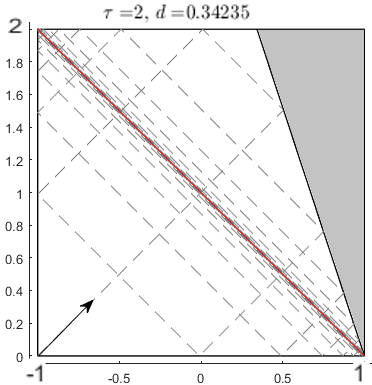
\includegraphics[scale=0.8]{Figs/CritAttrFreq.png}
    \caption{Вырожденный аттрактор внутренних волн.}
    \label{fig:trivAttr}
\end{figure}

Теперь найдем второй случай, при котором аттрактор зажимается между двумя противоположными углами. Это означает что луч пущенный из левого нижнего угла должен попасть в точку $d$. То есть $\tau = 1+d$:

\begin{equation}
    1+d=\frac{2H}{L} \sqrt{\frac{N^2}{\omega^2}-1}.
\end{equation}

Выразим отсюда частоту $\omega$:

\begin{equation}
    \omega = \frac{NH}{\sqrt{\left( 1-H\cdot tg(\alpha) \right)^2+H^2}}.
\end{equation}

После процедуры рейтрейсинга(см рис. \ref{fig:attrTriv})
    
\begin{figure}
    \centering
    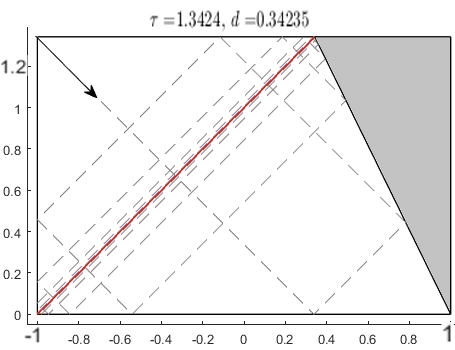
\includegraphics[scale=0.6]{Figs/AttrCritFreq.png}
    \caption{Вырожденный аттрактор внутренних волн.}
    \label{fig:attrTriv}
\end{figure}


Также с помощью метода спектральных элементов были смоделированы случаи вырожденных аттракторов (см. рис. \ref{fig:critNekfr}).

\begin{figure}
    \centering
    
    \begin{subfigure}[с]{1\textwidth}
        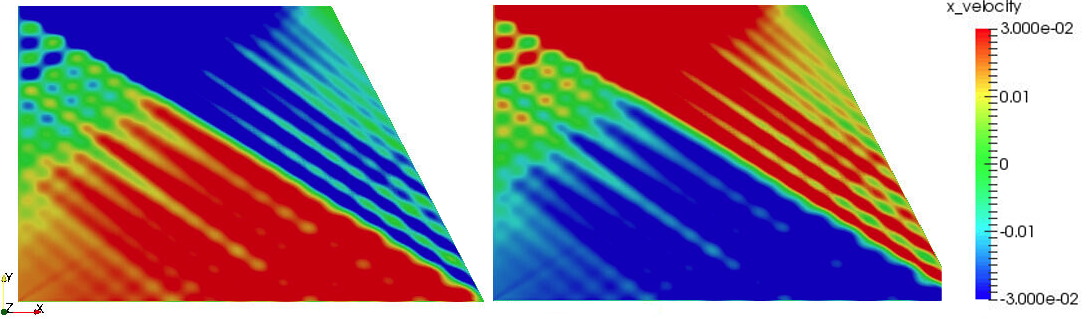
\includegraphics[scale=0.45]{Figs/AttrNEKcrit1.png}
        \caption{Расчет при помощи метода спектральных элементов с первой критической частотой}
    \end{subfigure}
    
    \begin{subfigure}[r]{1\textwidth}
        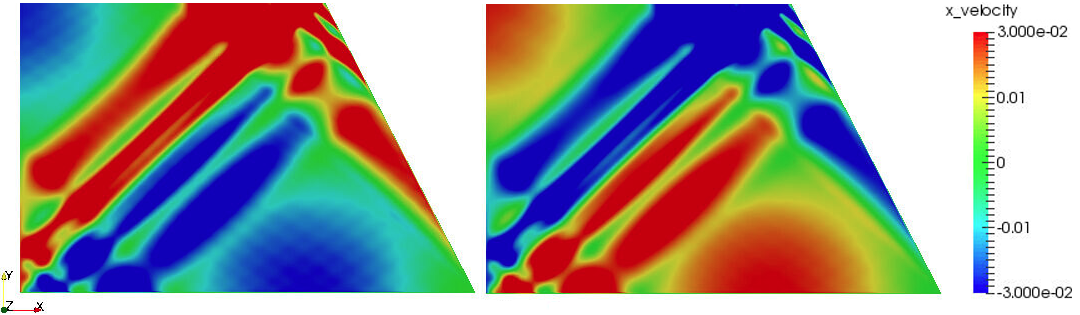
\includegraphics[scale=0.45]{Figs/AttrNekCrit2.png}
        \caption{Расчет при помощи метода спектральных элементов со второй критической частотой}
    \end{subfigure}
    \caption{Результаты расчетов при колебании волнопродуктора с критическими частотами}
    \label{fig:critNekfr}
\end{figure}

Критические значения замыкают собой диапазон частот, колебания волнопродуктора с которыми будет приводить к образованию аттрактора:

\begin{equation}
    \omega_{c_{1}}=\frac{NH}{\sqrt{L^2+H^2}}, \;\;\;\;\;\;\;\;\; \omega_{c_{2}} = \frac{NH}{\sqrt{\left( 1-H\cdot tg(\alpha) \right)^2+H^2}},
\end{equation}


\begin{equation}
    \omega_{c_{1}} \leq \omega_A \leq \omega_{c_{2}}.
\end{equation}


\section{Экспериментальные исследования}

Океан и атмосфера -- это естественные системы, обладающие стратификацией благодаря чему в них могут возникать внутренние волны. В этом разделе рассматриваются способы изучения внутренних волн в естественных условиях таких как в океане и атмосфере, а также методы воспроизвести эти условия экспериментально. Следует отметить, что в океане и атмосфере наблюдаются гравито-инерционные волны.

В лабораторных условиях рассматривается упрощенная модель, которая не учитывает эффекты связанные с вращением Земли, нелинейной стратификацией и сложной геометрией резервуара. Однако, рассматриваемые условия учитывают упрощенно основные характеристики океана. 

\subsection{Экспериментальная установка}

Экспериментальная установка представляет собой резервуар трапециевидной формы наполненный линейно стратифицированной жидкостью. Левая стенка резервуара является волнопродуктором, который производит внутренние волны. На рисунке \ref{fig:attrSetup} из \cite{Brouzet2016} изображена схема экспериментальной установки. Правая стенка наклонена на угол $\alpha$ с вертикальной стенки. Трапеция прямоугольная, с основанием $L$, высотой $H$ и глубиной $W$ вдоль оси $y$. 

\begin{figure}
    \centering
    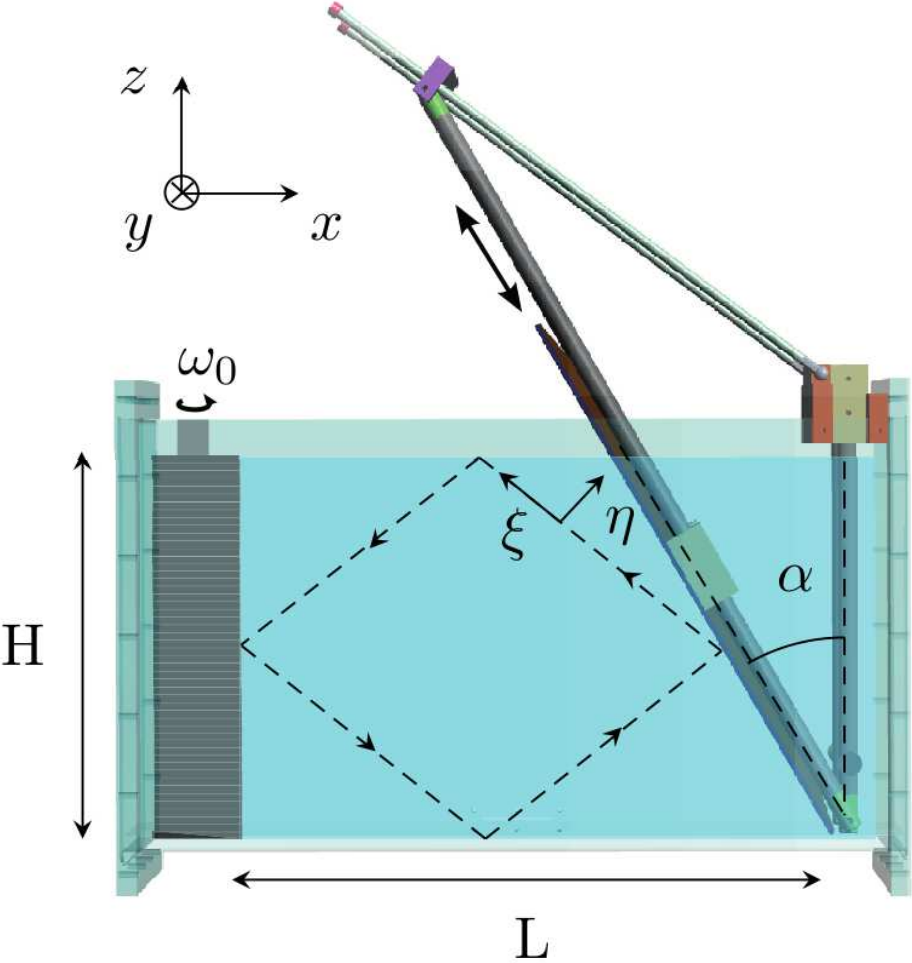
\includegraphics[scale=0.6]{pics/SetupAttr.png}
    \caption{Экспериментальная установка для воспроизведения эффекта многократной фокусировки внутренних волн. Взято из \cite{Brouzet2016}.}
    \label{fig:attrSetup}
\end{figure}

Установка для получения аттрактора внутренних волн расположена во Франции, город Лион. Внутренние волны продуцируются с помощью специального генератора. Исторически внутренние волны создавались в лаборатории путем колебания цилиндра в стратифицированной жидкости. Цилиндр создает четыре волновых луча в четырех квадрантах, как показано на рисунке \ref{fig:ermExp}. Так впервые было измерено дисперсионное соотношение для внутренних волн \cite{Grtler1943, Mowbray1967}.

Условия на левой стенке можно описать следующим уравнением:

\begin{equation}
    \zeta (z,t) = a \sin (\omega_0 t) \cos \left( \frac{\pi z}{H} \right) 
    \label{eq:wmOsc}
\end{equation}
где $a$ это амплитуда максимального смещения. 

Физически в эксперименте это достигается путем вращения дисков с эксцентриситетом в квадратных кожухах, схема изображена на рисунке. Диски размещены в разных фазах и согласованны друг с другом. Вращаясь диск сдвигает кожух, а кожух сдвигает жидкость. Профиль волнопродуктора в целом представляет собой полу косинус меняющий свою амплитуду во времени.

\begin{figure}
    \centering
    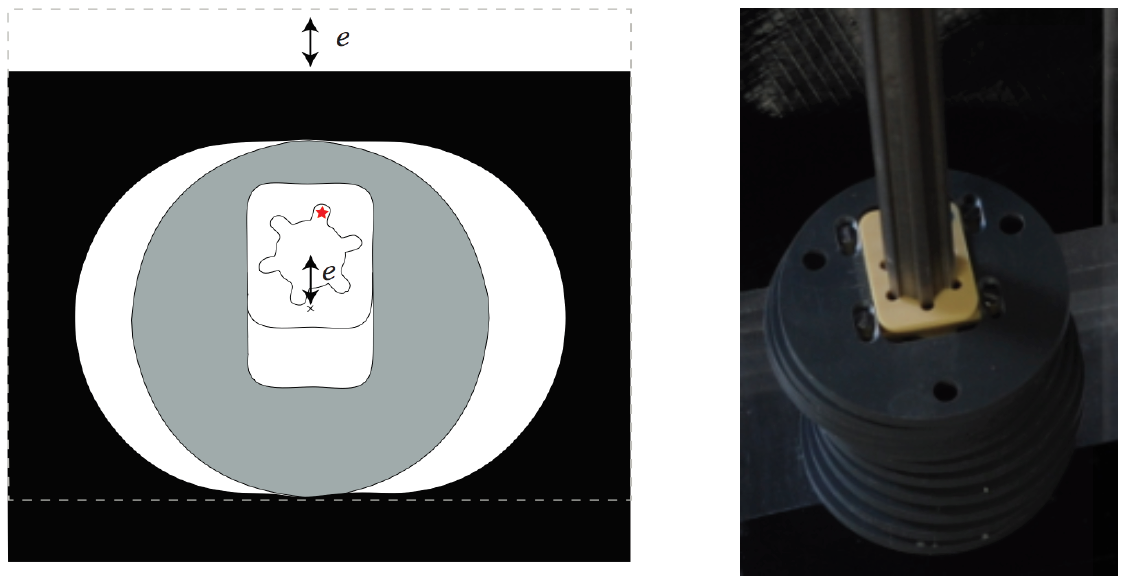
\includegraphics[scale = 0.5]{pics/wawemakerScheme.png}
    \caption{Устройство волнопродуктора для продуцирования внутренних волн в резервуаре наполненном стратифицированной жидкостью. Вращательное движение оси преобразуется в поступательное движение волнопродуктора. Изображение из \cite{Bordes2012InteractionsND, bourget, phdthesisGW}}
    \label{fig:WMrot}
\end{figure}

Такая конструкция волнопродуктора была разработана и описана в работе \cite{Gostiaux2006}, исследована \cite{MERCIER2010}, а в последствии и улучшена \cite{Bordes2012InteractionsND}. Такая конструкция позволяет очень тонко настраивать частоту амплитуду генерируемых волн.

Экспериментальная установка очень чувствительна из-за тонкой настройки стратификации. Поэтому сначала производится настройка волнопродуктора, установка фаз на дисках и амплитуд колебаний, затем резервуар заполняется водой, а потом туда аккуратно вставляется наклонная стенка под заданным углом. Регулировать после заполнения резервуара водой можно только частоту колебаний волнопродуктора. Для изменения других параметров придется заново наполнять резервуар. 

В \cite{Brouzet_2016} использовался несколько иной волнопродуктор. Идея его состоит в том, чтобы деформировать гибкую пластину, и таким образом получить закон колебания (\ref{eq:wmOsc}). На рисунке (\ref{fig:WMplate}) изображено устройство этого волнопродуктора. 

\begin{figure}
    \centering
    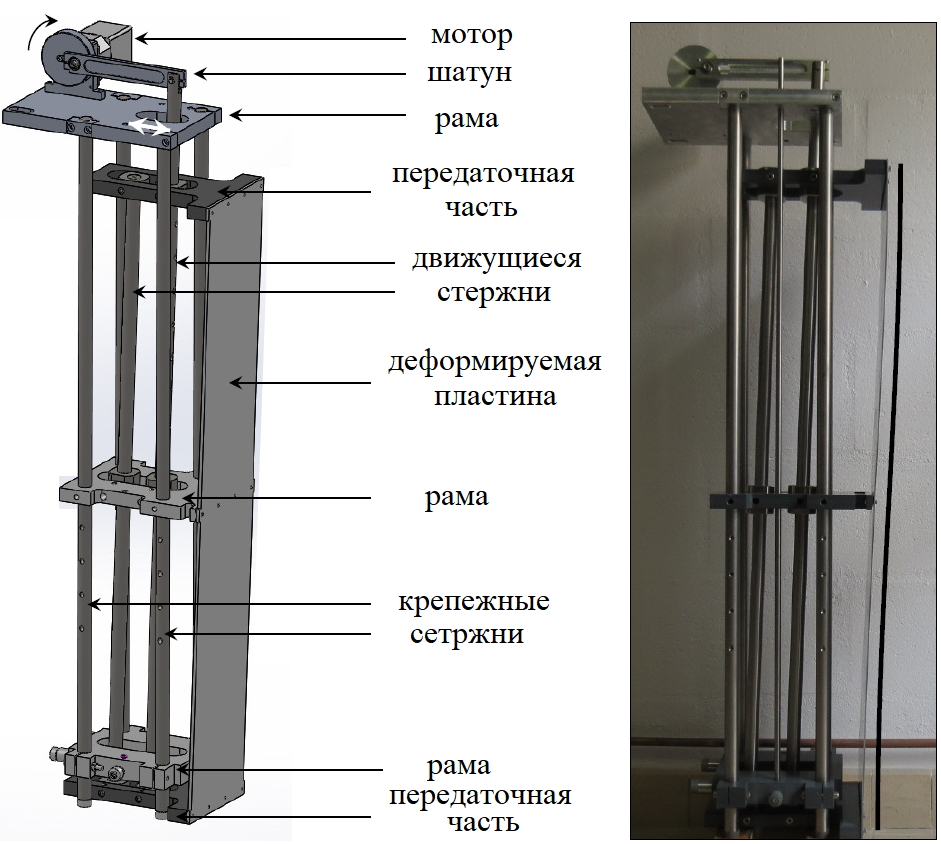
\includegraphics[scale=0.45]{pics/WMplate.png}
    \caption{Схема и фотография волнопродуктора используемого в Лионском эксперименте \cite{Brouzet_2016}}
    \label{fig:WMplate}
\end{figure}

Фиксированная часть волнопродуктора, состоит из трех различных горизонтальных частей, расположенных внизу, в середине и наверху волнопродуктора. Эти детали соединены четырьмя вертикальными стержнями. Деформируемая пластина прикреплена сверху и снизу к горизонтально перемещающимся деталям. Они движутся противофазно благодаря двум движущимся стержням по принципу деформируемого параллелограмма. Кроме того, середина пластины горизонтально прикреплена к раме, чтобы получить неподвижную точку в центре волнопродуктора. Верхняя и нижняя части двигаются поступательно благодаря двигателю в верхней части волнопродуктора. Пластина имеет ту же ширину $W$, что и резервуар, и герметизирована по бокам, чтобы избежать. Сплошная линия, имеющая форму половины косинуса, показывает, что деформация пластины очень близка к форме, которая задается формулой \ref{eq:wmOsc}. Можно изменить амплитуду колебаний, изменив стержень кривошипа после заполнения резервуара. Это позволяет проводить различные эксперименты, варьируя только амплитуду воздействия. Частоту воздействия также легко настроить, управляя двигателем.

Первые эксперименты с аттракторами внутренних волн датированы 1997 годом \cite{Maas1997}. Проведены в институте морских исследований в Нидерландах. Прямоугольный контейнер из плексигласа был заполнен экспоненциально расслоенным солевым раствором, так что частота плавучести была постоянной и составляла $N = 1.89 \; c^{-1}$. Контейнер имел трапециевидную форму в безразмерных геометрических парамерах $(\tau, d)$ $d=0$. Размеры были: глубина $(W)$ $96$ мм; высота $(H)$ $261$ мм; и длина $(L_1)$ $261$ мм. Жидкость подкрашена для визуализации внутренних волн. Краситель периодически впрыскивается в раствор, маркируя частицы жидкости заданной плотности. Вертикальная лазерная плоскость подсвечивает деформацию полосок красителя.

Внутренние волны в этом эксперименте возбуждаются колебаниями всего резервуара с частотой $\omega$ и амплитудой $a$. Тогда любая волна с частотой q параметрически усиливается. Волны повсюду возбуждаются с одинаковой фазой, задаваемой воздействием. Примерно через пять минут после начала колебания становится видимым двумерное колебательное движение линий красителя с частотой $\omega / 2$. Это колебание локализовано, принимает форму параллелограмма и наиболее ярко проявляется вокруг предсказанного с помощью трассировки лучей местоположения. 

\begin{figure}
    \centering
    \begin{subfigure}[t]{0.45\textwidth}
        \centering
        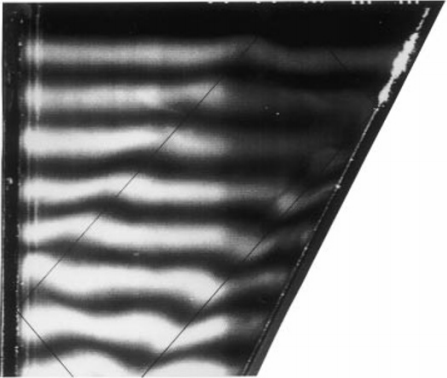
\includegraphics[scale=0.6]{pics/Exp1997Maas.png}
        \caption{предсказанная форма аттрактора с помощью метода трассировки лучей}
        \label{fig:maasExperA}
    \end{subfigure}
    \begin{subfigure}[t]{0.45\textwidth}
        \centering
        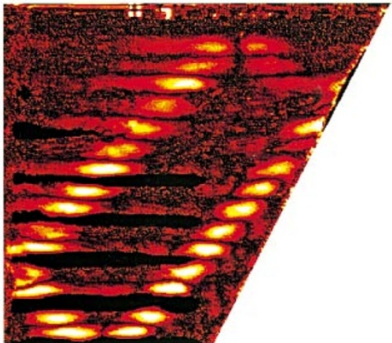
\includegraphics[scale=0.67]{pics/Exp1997MaasB.png}
        \caption{Визуализированные колебания стратифицированной жидкости после фокусировки}
        \label{fig:maasExperB}
    \end{subfigure}
    \caption{Нидерландский эксперимент проведенный Лео Маасом в 1997 году \cite{Maas1997}}
    \label{fig:maasEper1997}
\end{figure}

Затем были проведены эксперименты описанные в \cite{Brouzet_2016,Brouzet2016,brouzet1997laboratory} с волнопродукторами, изображенными на рисунках \ref{fig:WMplate} и \ref{fig:WMrot}. 

В России эксперименты со стратифицированной жидкостью проводятся Евгением Ерманюком \cite{Shmakova2019}. В числе экспериментов опыты с генерированием внутренних волн \cite{Shmakova2017} и фокусировкой в тороидальном резервуаре \cite{Ermanyuk2017}.  

\section{Численные исследования}

Помимо экспериментальных исследований в лабораторных условиях проводятся и исследования численные. Одной из самых успешных практик численного моделирования аттракторов внутренних волн является моделирование при помощи метода спектральных элементов \cite{Brouzet2016} и его конкретной реализации \cite{NEK5000}. Очевидные преимущества этого метода -- скорость и точность расчетов. Недостатки также имеются.

Второй способ моделирования течения стратифицированной жидкости -- метод конечного объема и его конкретная реализация openFOAM \cite{OpenFOAM}. Попытки моделирования были проведены в 2014м году \cite{Brouzet2014}. Очевидные достоинства этого метода и реализации -- гибкость, понятность и подробная документация исходного кода. Однако и этот пусть не обделен недостатками.

В работе рассматриваются различные конфигурации расчетной области (Рис. \ref{fig:dominleft},\ref{fig:domainup}).

\begin{figure}[!ht]
        \centering
          \begin{tikzpicture}[scale=1.0, z={(-.707,-.5)}]
            \draw (0,0,0) -- (6,0,0) -- (4,4,0)--(0,4,0) --cycle;
            \draw (0,0,0)     -- (6,0,0)   -- (4,4,0)   -- (0,4,0)    -- cycle;
            \draw[style = dashed] (2.7,4,0)   -- (0,1.8,0) -- (2.2,0,0) -- (5,2.1,0)-- cycle;
            %\draw[style = dashed] (0,0.985,0) -- (3.3,4,0) -- (4.5,3,0) -- (1.1,0,0)  -- cycle;

            \draw[<->] (-0.1,0) --node[above,rotate=90] {$H = 40$ cm} (-0.1,4);
            \draw[<->] (0,-0.1,0) --node[below,] {$L_2 = 60$ cm} (6,-0.1,0);
            \draw[<->] (0,4.1,0) --node[above,] {$L_1 = 40$ cm} (4,4.1,0);

            \draw[color=red] (3.0,0)--(3.0,4.0);
            
            \draw (3.15,0) node[above] {$A$};
            \draw (3.15,4.0) node[below] {$B$};

            \draw[thick,->] (4.95,3.5,0) -- (5.95,3.5,0) node[anchor=north east]{$x$};
            \draw[thick,->] (4.95,3.5,0) -- (4.95,4.5,0) node[anchor=north west]{$z$};
            \draw[thick,->] (5.3,3,0) -- (5.3,2,0) node[anchor=west]{$\vec{g}$};
          \end{tikzpicture}
          \caption{Вычислительная область для аттракторов внутренних волн, красным показана линия пробы, пунктиром показана предполагаемая форма аттрактора}
          \label{fig:dominleft}
\end{figure}

\begin{figure}[!ht]
    \centering
    \begin{tikzpicture}[scale=1, z={(-.707,-.5)}]
    \draw (3.6,0,0) -- (0,0,0) -- (0,4,0)--(6,4,0)--(3.6,0,0);
    %\draw (3.6,0,0) -- (3.6,0,-1) -- (6,4,-1) -- (6,4,0) -- cycle;
    %\draw (6,4,0) -- (0,4,0) -- (0,4,-1) -- (6,4,-1);
    \draw (-0.5,2,0) node{};
    \draw (4.1,-.2,-1.5) node{};
    \draw (3.5,5,0) node{};
    \draw[<->] (-0.1,0) --node[above,rotate=90] {$H = 40$cm} (-0.1,4);
    \draw[<->] (0,4.1,0) --node[above,] {$L_1 = 60$ cm} (6,4.1,0);
    \draw[<->] (0,-0.1,0) --node[below,] {$L_2=36.9$ cm} (3.6,-0.1,0);
    \draw [black, thick] (5.5,4) arc [start angle=180, end angle=240, radius=0.5cm]
        node [left] {$60^\circ$};
    \draw[thick,->] (5.5,1,0) -- (6.5,1,0) node[anchor=north east]{$x$};
    \draw[thick,->] (5.5,1,0) -- (5.5,2,0) node[anchor=north west]{$z$};
    \draw[thick,->] (3,3,0) -- (3,1,0) node[anchor=west]{$\vec{g}$};
    \end{tikzpicture}
    \caption{Конфигурация вычислительной области для аттрактора внутренних гравитационных волн}
    \label{fig:domainup}
\end{figure}

Принципиальной разницы в этих двух вариантах нет в первом случае волнопродуктор располагается на левой стенке, а во втором сверху.

\subsection{Численное моделирование аттракторов внутренних волн с помощью метода спектральных элементов}

Метод спектральных элементов\cite{Patera1984}. Результаты полученные при помощи метода спектральных элементов были достаточно близки к результатам натурных экспериментов\cite{Brouzet2016,Brouzet_2016}. Недостатком метода является отсутствие реализаций с открытым исходным кодом позволяющие встроить дополнительные физические модели и проводить расчеты на сложной геометрии приближенной к реальной топологии океанического дна.

Используемая реализация -- пакет с открытым исходным кодом nek5000\cite{NEK5000}. 

В методе спектральных элементов решение и данные представлены в виде полиномов тензорного произведения $N$-го порядка внутри каждого из $E$ деформируемых шестигранных (кирпичных) элементов. Типичные дискретизации включают $E = 100 - 10 000$ элементов порядка $N = 8 - 16$ (что соответствует $512 - 4096$ точкам на элемент). Векторизация и эффективность кеширования проистекают из локального лексикографического упорядочения в каждом макроэлементе и из того факта, что действие дискретных операторов, которые номинально имеют $O(E\cdot N \cdot 6)$ ненулевых значений, может быть оценено только за $O(E\cdot N \cdot 4)$ и $O(E\cdot N\cdot 3)$. хранение за счет использования факторизации тензор-произведение-сумма. Метод спектральных элементов демонстрирует очень небольшую числовую дисперсию и диссипацию, что может быть важно, например, при расчетах устойчивости, для длительного интегрирования и для потоков с большим числом Рейнольдса.

Nek5000 решает нестационарные несжимаемые двумерные, осесимметричные или трехмерные уравнения Стокса или Навье-Стокса с вынужденной или естественной конвекцией теплопередачи как в стационарной (фиксированной), так и в движущейся геометрии. Он также решает уравнение Навье-Стокса для сжимаемой жидкости при низких числах Маха.

На данный момент это самый точный способ численно воспроизвести экспериментальные данные\cite{Brouzet2016,Brouzet_2016}. Недостаток реализации заключается в том, что геометрия задается путем аффинных преобразований. Подобрать преобразование, которое отображало бы прямоугольник в сложную геометрию океанического дна представляется трудоемкой задачей. 

Для моделирования методом спектральных элементов используется конфигурация расчетной области представленная на рисунке \ref{fig:domainup}. На протяжении всего эксперимента на верхней стенки задается граничное условие для скорости:

\begin{equation}
    U_z = A\cdot cos\left(\frac{\pi \cdot z}{L_1}\right)\cdot \omega \cdot  sin(\omega_0 t)
\end{equation}

Где $\omega_0$ -- частота волнопродуктора. 

На остальных стенках для скорости:

\begin{equation}
    \vec{U} = 0
\end{equation}

Граничные условия для давления на стенках:

\begin{equation}
    \nabla p = 0
\end{equation}

Условие для градиента солености на стенках:

\begin{equation}
    \frac{\partial s}{\partial n} = grad(s_0)
\end{equation}

$s_0$ -- начальное распределение солености в резервуаре.

\begin{figure}[!ht]
    \centering
    \begin{subfigure}[с]{0.45\textwidth}
        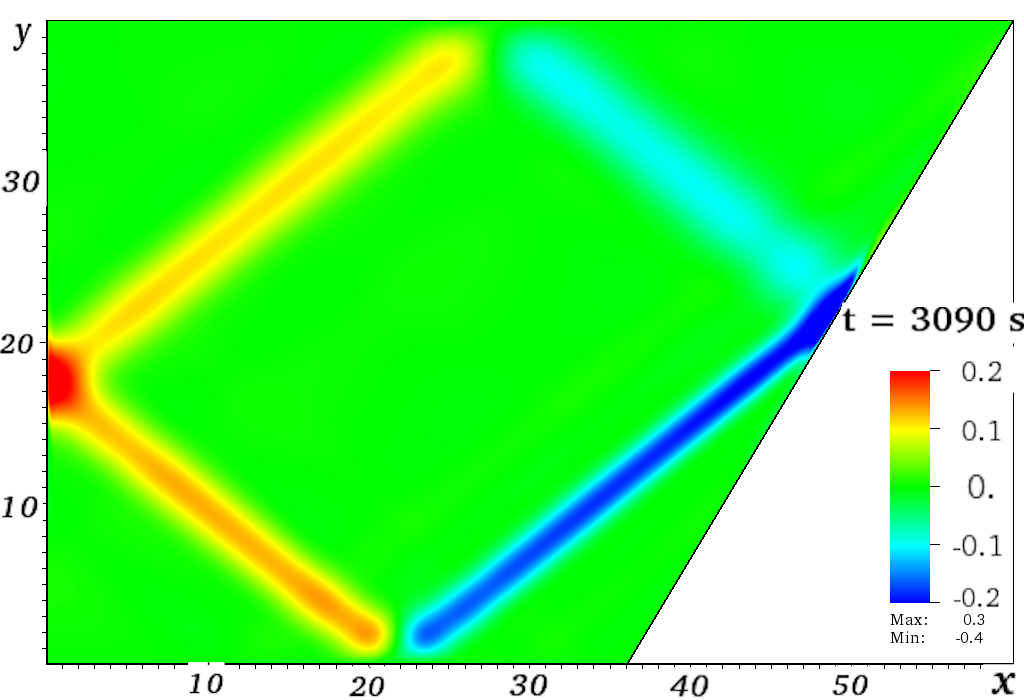
\includegraphics[scale=0.15]{pics/H40L60N1ap02dp20w0p63/2D36x36DiagramH40L60N1ap02dp20w0p63Vyn06179.png}
        \caption{Горизонтальная компонента скорости}
    \end{subfigure}
    \begin{subfigure}[с]{0.45\textwidth}
        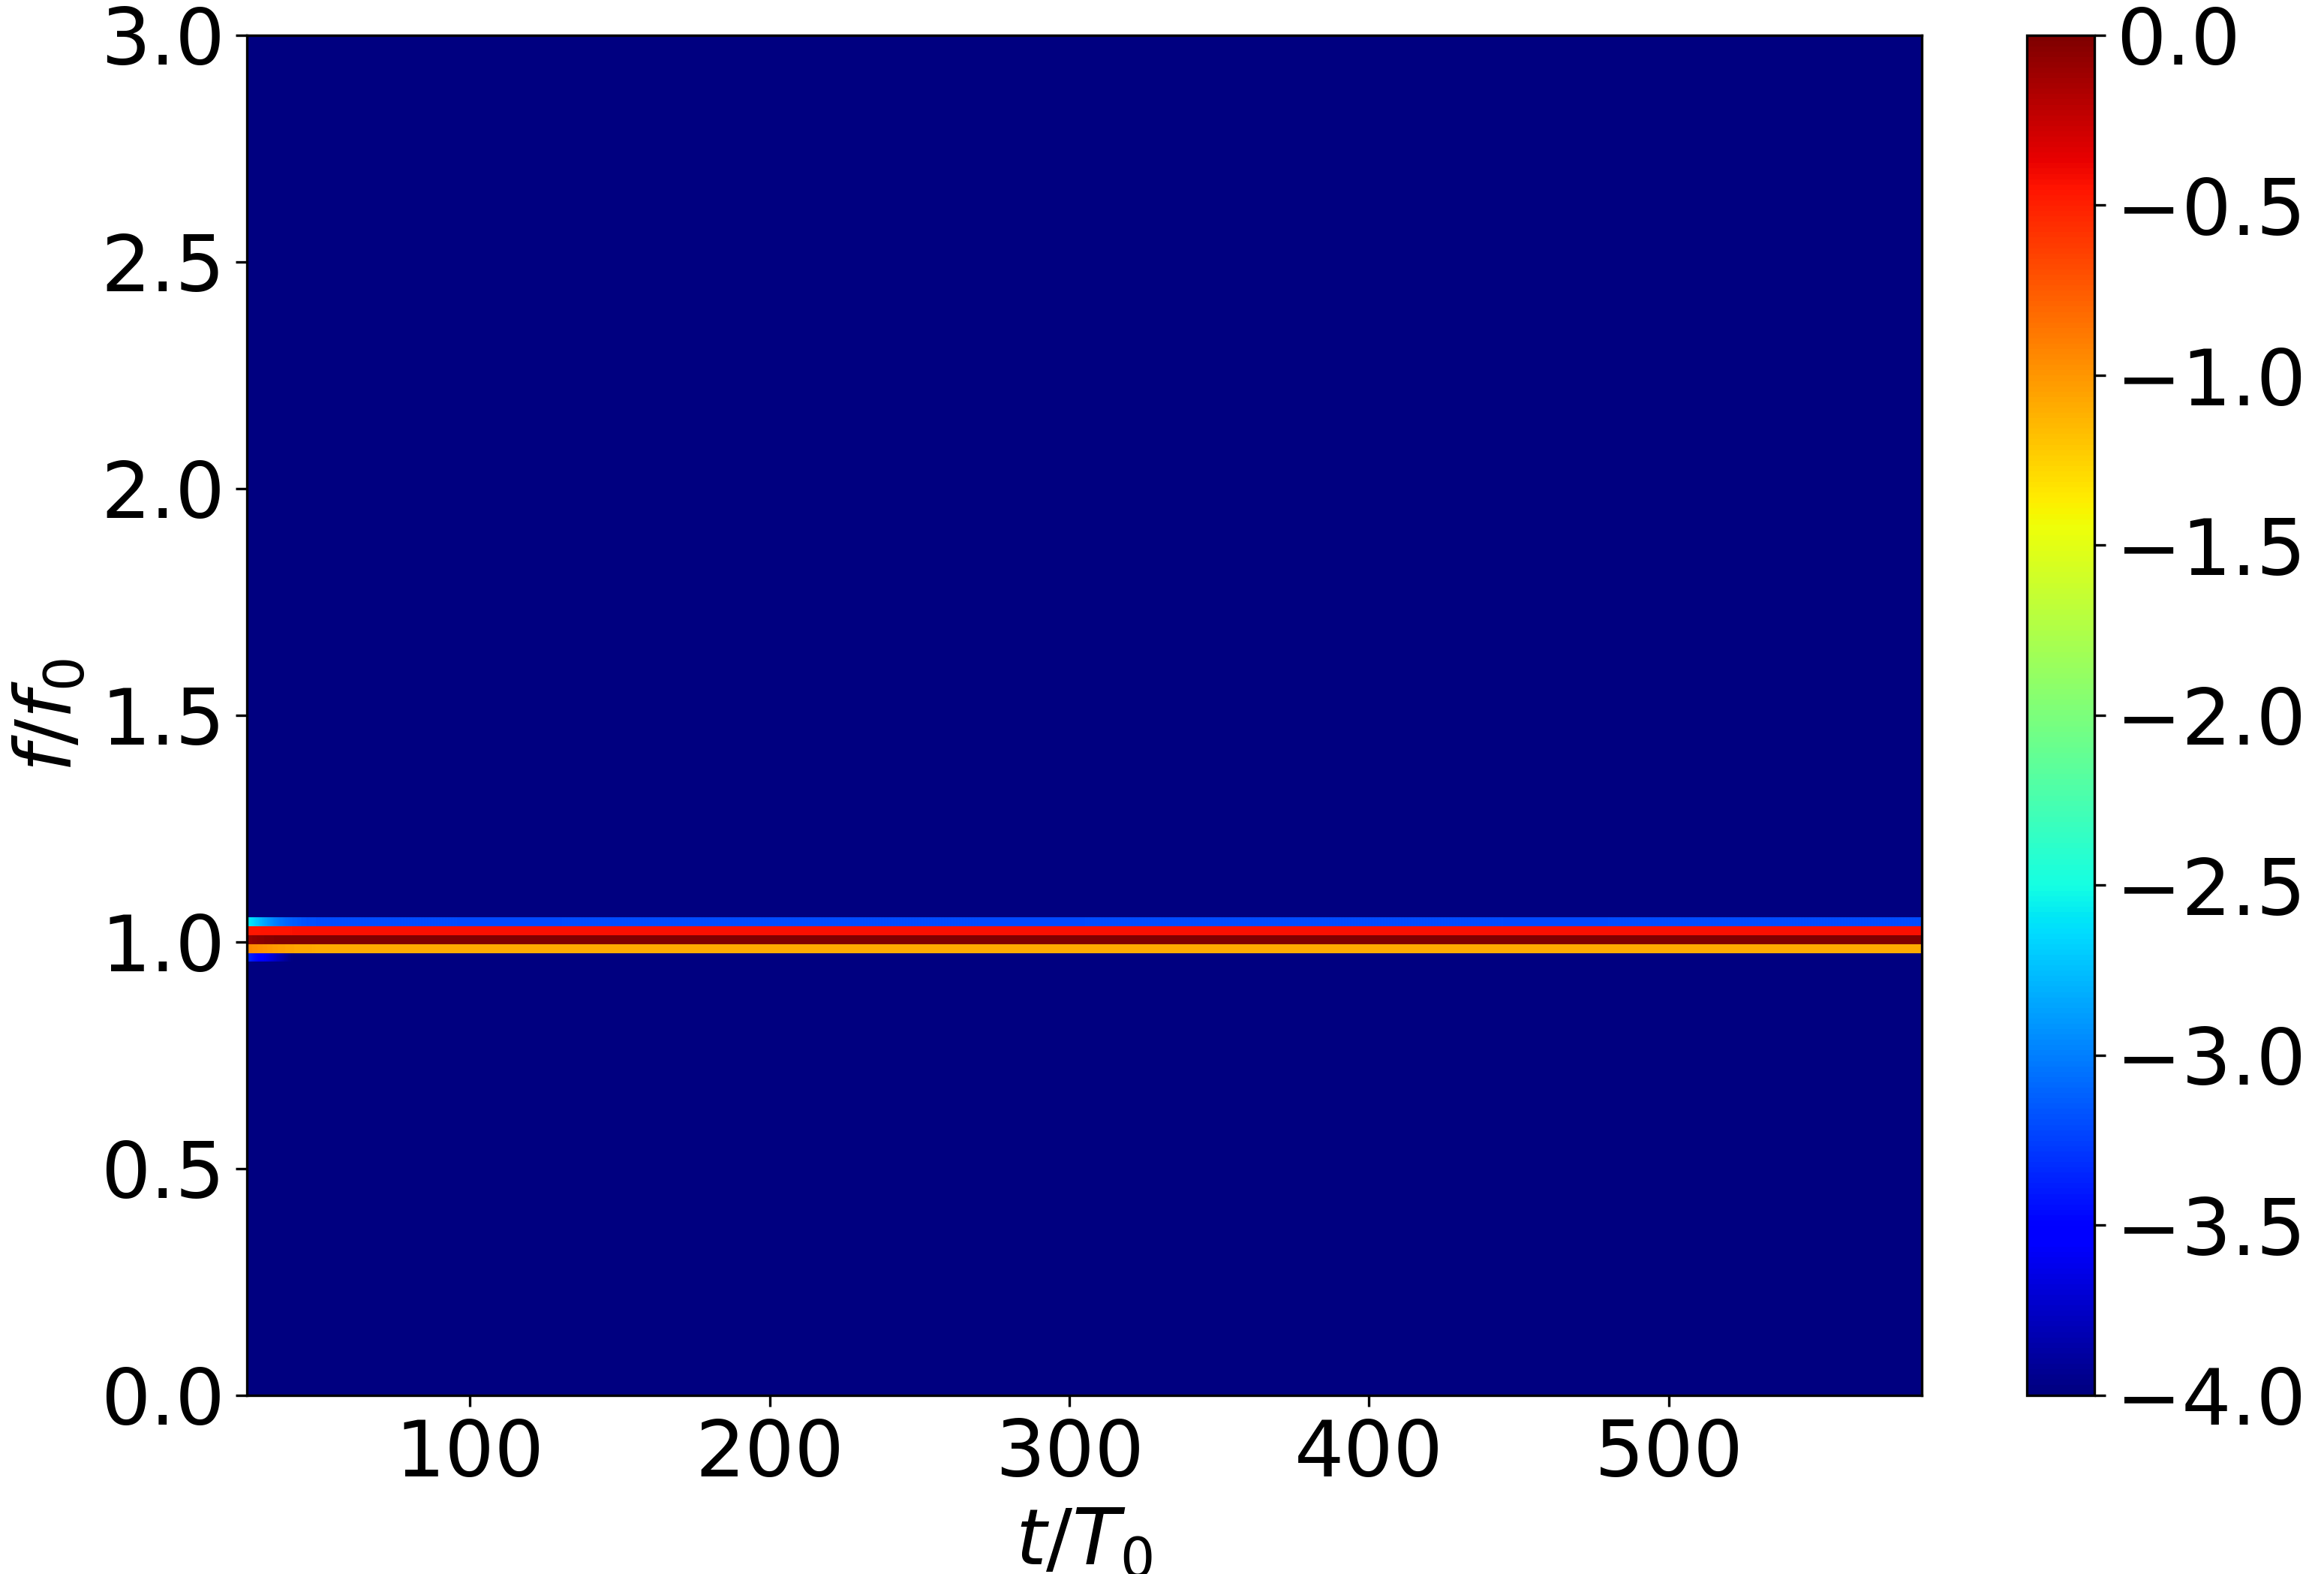
\includegraphics[scale=0.07]{pics/H40L60N1ap02dp20w0p63/TFspectrumX356Y112N1024.png}
        \caption{Частотно-временная диаграмма на аттракторе}
    \end{subfigure}
    \begin{subfigure}[с]{0.45\textwidth}
        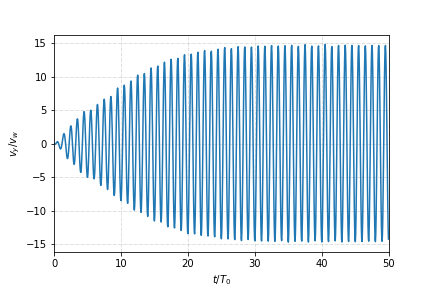
\includegraphics[scale=0.5]{pics/H40L60N1ap02dp20w0p63/vyX355662118341Y112748618745t1000.png}
        \caption{Амплитуда скорости в зависимости от времени на аттракторе}
    \end{subfigure}
    \begin{subfigure}[с]{0.45\textwidth}
        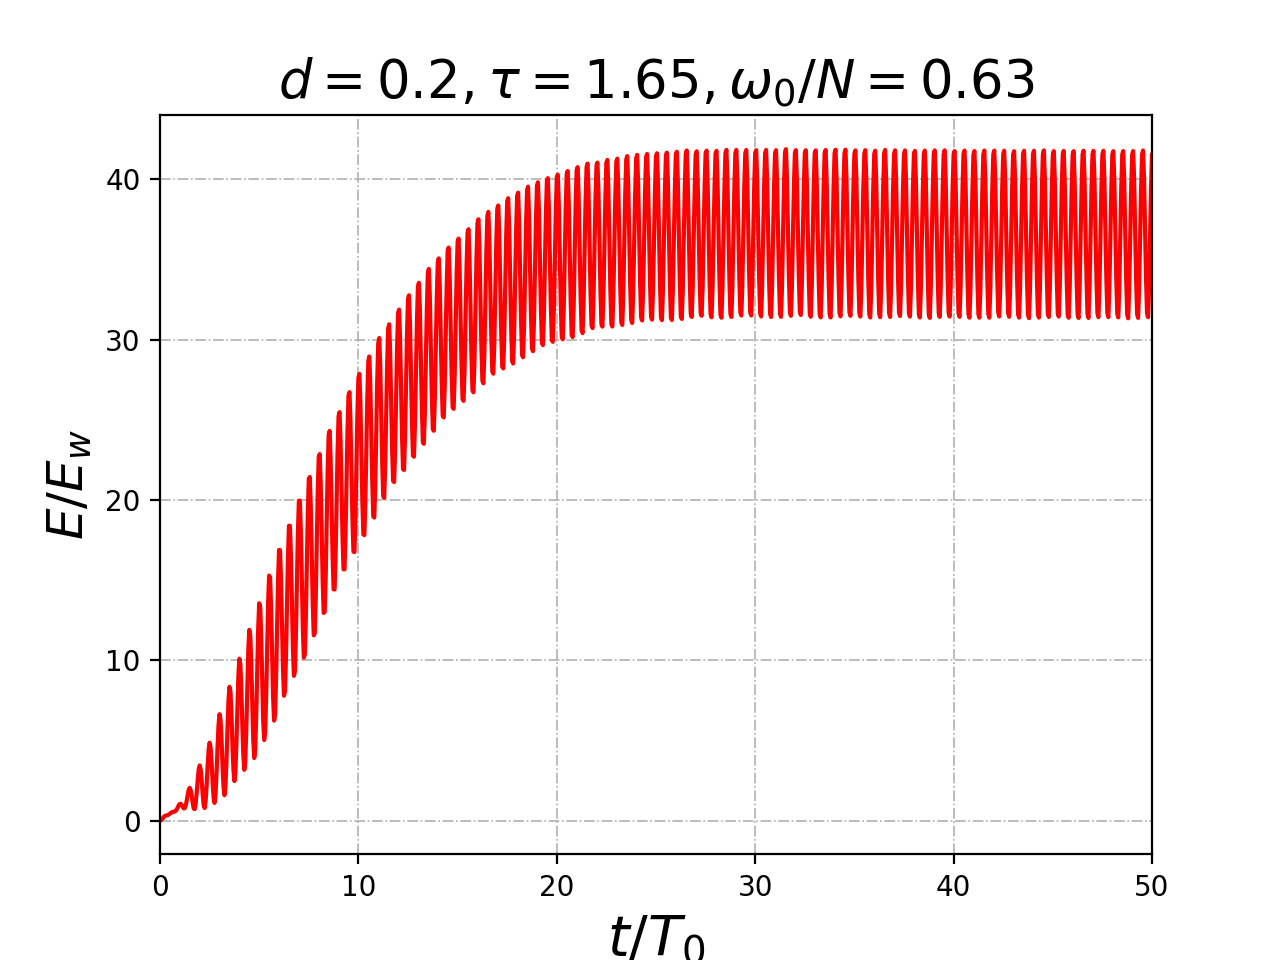
\includegraphics[scale=0.4]{pics/H40L60N1ap02dp20w0p63/2D36x36DiagramH40L60N1ap02dp20w0p63totKEnonDim.png}
        \caption{Средняя кинетическая энергия в резервуаре}
    \end{subfigure}
    
    \caption{Результат моделирования аттрактора внутренних волн методом спектральных элементов}

\end{figure}

В заключении можно сказать, что алгоритм высокого порядка точности хорошо воспроизводит результаты натурного эксперимента. В дальнейшем они будут использоваться как эталон для сравнения с остальными методами решения. 

\subsection{Численное моделирование аттракторов внутренних волн с помощью метода контрольного объема}

Для моделирования методом конечного объема используется конфигурация представленная на рисунке \ref{fig:dominleft} в этом случае волнопродуктор установлен на левой стенке и колеблется по следующему правилу:

\begin{equation}
    U_x = A\cdot cos\left(\frac{\pi \cdot z}{H}\right)\cdot \omega \cdot  sin(\omega_0 t)
\end{equation}

Аналогично условия на остальных стенках:

\begin{equation}
    \vec{U} = 0
\end{equation}

Для давления:

\begin{equation}
    \nabla p = 0
\end{equation}

Для градиента солености:

\begin{equation}
    \frac{\partial s}{\partial n} = grad(s_0)
\end{equation}

Уравнения движения стратифицированной жидкости (\ref{eq:momClassic} - \ref{eq:contClassic}) представляются в виде дискретных аналогов. Аналог производной по времени:

\begin{equation}\label{eq:qhd_Euler}
    \frac{\partial \vec{U}}{\partial t} \approx \frac{ \vec{U}^n-\vec{U}^o}{\Delta t}, \,\,\,  \frac{\delta \vec{U}}{\delta t} =  \frac{ \vec{U}^n-\vec{U}^o}{\Delta t},
\end{equation}
разностный аналог уравнения движения:

\begin{multline}\label{eq:qhd_approx_momentum}
    \frac{\delta \vec{U}}{\delta t} + \frac{1}{V} \sum_f \vec{S}_f \cdot \vec{U}^o_f \otimes \vec{U}^n_f  - \frac{1}{V} \sum_f \nu_f \frac{\delta\vec{U}^n}{\delta \vec{n}_f} |\vec{S}_f| - \frac{1}{V} \sum_f \nu_f \vec{S}_f \cdot [\nabla \vec U^o]_f^T = \\
    = - \frac{1}{\rho_0} \frac{1}{V} \sum_f \tilde p^o_f \vec S_f + \vec{F}^o,
\end{multline}
и аналог уравнения неразрывности:

\begin{equation}
    \sum_f \vec{S_f} \cdot \vec{U}_f^n = 0.
\end{equation}

Производные по направлению вычисляются согласно шаблону приведённому на рис. \ref{qhd}:

\begin{equation}
    \vec{U}_w^n= \frac{\vec{U}_W^n-\vec{U}_P^n}{|\vec{d}_f|}|\vec{d}|+\vec{U}_P, \,\,\, \frac{\delta\vec{U}^n}{\delta \vec{n}_w} = \frac{\vec{U}^n_P-\vec{U}^n_W}{|\vec{d}|},
\end{equation}

\begin{figure}
    \centering
    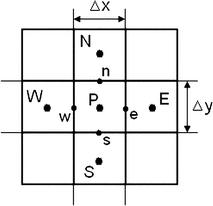
\includegraphics{pics/b701170a-f6.jpeg}
    \caption{Расчетный шаблон для метода конечных элементов}
    \label{qhd}
\end{figure}

В качестве алгоритма нахождения численного решения используется PISO \cite{IssaGosmanWatkins-PISO}. Вкратце изложить алгоритм нахождения полей скорости и давления можно так:

\begin{enumerate}[1.]
    \item Устанавливаются граничные условия.
    \item Решается дискредитированное уравнение движения для вычисления промежуточных значений поля скорости.
    \item Вычисляются массовые потоки через границы ячеек.
    \item Решается уравнение для давления.
    \item Корректируются массовые потоки.
    \item Корректируется поле скорости согласно новому давлению.
    \item Обновляются граничные условия.
    \item Вернуться к третьему шагу.
    \item Перейти на следующий временной шаг и начать с первого пункта.
\end{enumerate}

Внутри шага по времени имеется цикл между пунктом 3 и пунктом 8. Более того возможны коррекции неортогональности ячеек сетки если зациклить этот алгоритм между пунктом 4 и 5. дискредитированное уравнение движение в матричном виде можно записать следующим образом: 

\begin{equation}
    \left[
        \begin{array}{cccc}
            m_{11} & m_{12} & \ldots & m_{1n}\\[0.055cm]
            m_{21} & m_{22} & \ldots & m_{2n}\\[0.055cm]
            \vdots & \vdots & \ddots & \vdots\\[0.055cm]
            m_{n1} & m_{n2} & \ldots & m_{nn}
        \end{array}
        \right]
        \left[
        \begin{array}{c}
            \vec{U}_{1}^* \\[0.1cm] 
            \vec{U}_{2}^* \\[0.1cm]
            \vdots \\[0.1cm]
            \vec{U}_{n}^*  
        \end{array}
        \right]
        =
        \left[
        \begin{array}{c}
            \vec{R}_{1} \\[0.1cm] 
            \vec{R}_{2} \\[0.1cm]
            \vdots \\[0.1cm]
            \vec{R}_{n}  
        \end{array}
    \right],
\end{equation}

или в полудискретной записи:

\begin{equation}
    \mathcal{M} \vec{U}^* = -\frac{\nabla p}{\rho_m} + \vec{F}.
\end{equation}

Где матрица  $\mathcal{M}$ состоит из коэффициентов   которые вычисляются как сумма потоков через соответствующие грани контрольного объема. $\vec{U}^*$ -- искомые промежуточные значения поля скоростей. Для получения уравнения давления эта матрица коэффициентов расщепляется следующим образом:

\begin{equation}
    \left[
        \begin{array}{cccc}
            m_{11} & m_{12} & \ldots & m_{1n}\\[0.055cm]
            m_{21} & m_{22} & \ldots & m_{2n}\\[0.055cm]
            \vdots & \vdots & \ddots & \vdots\\[0.055cm]
            m_{n1} & m_{n2} & \ldots & m_{nn}
        \end{array}
        \right]
        \left[
        \begin{array}{c}
            \vec{U}_{1}^* \\[0.1cm] 
            \vec{U}_{2}^* \\[0.1cm]
            \vdots \\[0.1cm]
            \vec{U}_{n}^*  
        \end{array}
        \right]
        =
        \left[
        \begin{array}{c}
            \vec{H}_{1} \\[0.1cm] 
            \vec{H}_{2} \\[0.1cm]
            \vdots \\[0.1cm]
            \vec{H}_{n}  
        \end{array}
        \right]
        -
        \left[
        \begin{array}{c}
            \frac{\nabla p_1}{\rho_m} \\[0.1cm] 
            \frac{\nabla p_2}{\rho_m} \\[0.1cm]
            \vdots \\[0.1cm]
            \frac{\nabla p_n}{\rho_m}
        \end{array}
        \right],
\end{equation}

или в полудискретной записи:

\begin{equation}
    \mathcal{M} \vec{U}^* = \mathcal{A} \vec{U}^* - \mathcal{\vec{H}},
\end{equation}
где $\mathcal{\vec{H}}$ -- источниковые члены для уравнения давления. $\mathcal{A}=diag(\mathcal{M})$. Подставляем расщепленную матрицу коэффициентов в уравнение движение:
\begin{equation}
    \mathcal{A} \vec{U}^* - \mathcal{\vec{H}}= -\frac{\nabla p}{\rho_m} + \vec{F}    
\end{equation}
Умножаем обе части на $\mathcal{A}^{-1}$, выражаем $\vec U$

\begin{equation}
    \mathcal{A}^{-1} \mathcal{A} \vec{U} = \mathcal{A}^{-1} \mathcal{\vec{H}} - \mathcal{A}^{-1} \nabla p + \mathcal{A}^{-1} \vec{F} \;\;=>\;\;
    \vec{U} = \mathcal{A}^{-1} \mathcal{\vec{H}} - \mathcal{A}^{-1} \nabla p + \mathcal{A}^{-1} \vec{F}
\end{equation}
согласно уравнению неразрывности $\nabla \vec{U} = 0$, это дает нам уравнение для давления:

\begin{equation}
    \nabla \cdot (\mathcal{A}^{-1} \nabla p) = \nabla \cdot (\mathcal{A}^{-1} \mathcal{\vec{H}} + \mathcal{A}^{-1} \vec{F})
\end{equation}

Алгоритм PISO не прост в понимании и сложен из-за двух вложенных циклов внутри одного временного шага. Но очень популярен и долгое время остается одним из самых востребованных инструментов вычислительной  гидродинамики. Блок-схема алгоритма проиллюстрирована на рис. \ref{fig:blockSchemePIMPLE}

\begin{figure}[h]
    \tikzstyle{decision} = [diamond, draw, 
    text width=4.5em, text badly centered, node distance=2cm, inner sep=0pt, minimum width=10em]
    \tikzstyle{block} = [rectangle, draw
    %, text width=30em
    , text centered, minimum height=2em, node distance=1.5cm
    %,minimum width=30em
    ]
    \tikzstyle{line} = [draw, -latex']
    \tikzstyle{cloud} = [draw, ellipse,fill=red!20, node distance=4cm,
    minimum height=2em]
    \centering
    \begin{tikzpicture}[node distance = 2cm, auto,scale = 1]
    % Place nodes
        \node [block] (UpdateF) {Начало};
        
        \node [block, below of=UpdateF] (Control) {Вчисление потоков};
        \node [block, below of=Control] (Stability) {Решение уравнения движения};
        \node [block, below of=Stability] (Increasing) {Решение уравнения давления с учетом неортогональности};
        \node [block, below of=Increasing] (Store) {Обновление давления и скорости};

        \node [decision, below of=Store] (Pressure) {PISO?};
        \tikzstyle{block} = [rectangle, draw, text centered, minimum height=2em, node distance=2.5cm]
        \node [block, below of=Pressure] (Salinity) {Обновление оператора при уравнении движения};
        
        \tikzstyle{block} = [rectangle, draw, text centered, minimum height=2em, node distance=1.5cm]    
        
        \node [block, below of=Salinity] (SolvePressure) {Решение уравнения давления с учетом неортогональности};
        

        %\tikzstyle{decision} = [diamond, aspect=2,draw, text width=10em, text badly centered, node distance=2cm, inner sep=0pt, minimum width=2em,minimum height=2em]
       % \node [decision, below of=Salinity] (NoNOrth) {Non-orthogonal corrections?};
        \tikzstyle{block} = [rectangle, draw, text centered, minimum height=2em, node distance=1.7cm]
        \node [block, below of=SolvePressure] (pressureUpd) {Обновление давления и скорости};
        \tikzstyle{block} = [rectangle, draw, text centered, minimum height=2em, node distance=1.7cm]
        \node [block, below of=pressureUpd] (solveOther) {Решение уравнения переноса};
        
        \node [decision, below of=solveOther] (conv){Сошлось?};
        \tikzstyle{block} = [rectangle, draw, text centered, minimum height=2em, node distance=2.5cm]
        \node [block, below of=conv] (end) {Конец};
        \tikzstyle{block} = [rectangle, draw, text centered, minimum height=2em, node distance=2cm]


        \path [line,distance = 5cm] (UpdateF) -- (Control);
        \path [line] (Control) -- (Stability);
        \path [line] (Stability) -- (Increasing);
        \path [line] (Increasing) -- (Store);
        \path [line] (Store) -- (Pressure);
        \path [line] (Pressure) -- node {да} (Salinity);
        \path [line] (Pressure) -| node [near start] {нет} ($(solveOther.west)-(4,0)$) -- (solveOther.west);

        %\path [line] (Salinity) -- (pressureUpd);
        \path [line] (Salinity) -- (SolvePressure);
        \path [line] (SolvePressure) -- (pressureUpd);
        %\path [line] (NoNOrth) -- node {no} (pressureUpd);
        %\path [line] (NoNOrth) -| node[near start] {yes} ($(Increasing.east)+(2,0)$) -- (Increasing.east);
        \path [line] (pressureUpd) -- (solveOther);
        \path [line] (solveOther) -- (conv);
        \path [line] (conv) -- node {да} (end);
        \path [line] (conv) -| node[near start] {нет} ($(Control.east)+(5,0)$) -- (Control.east);
        %path [line] (setValues.north) -| ($(Control.east)+(1.45,0)$) -- (Control.east);
    \end{tikzpicture}
    
    \caption{Схема алгоритма PISO}
    \label{fig:blockSchemePIMPLE}
\end{figure}

К сожалению, результаты моделирования аттрактора внутренних волн алгоритмом PISO количественно не соответствуют результатам полученным при помощи метода спектральных элементов. 

Подведя итог можно сказать следующее, популярный алгоритм качественно воспроизводит картину течения, образующуюся при многократном отражении внутренних волн от стенок трапециевидного резервуара. Но количественно нет. Преимуществом алгоритма является способность работать с неортогональными сетками и сложной геометрией. К недостаткам можно отнести сложность и нелинейность процедуры нахождения гидродинамических полей.

\begin{figure}[!ht]
    \centering
        \begin{tikzpicture}[scale=5.34, z={(-.707,-.5)}]
          \node[anchor=south west,inner sep=0] at (0,0) {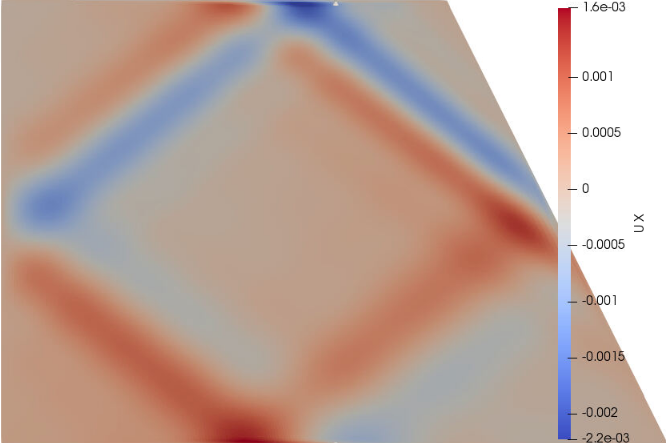
\includegraphics[width=\textwidth]{Figs/Attr200s.png}};
          \draw[thick,style = dashed] (1.5, 0, 0) -- (1.5, 2, 0);
        \end{tikzpicture}
    \caption{Поле горизонтальной компоненты скорости, пунктиром показана линия пробы}
    \label{fig:attractorRes}
\end{figure}

\begin{figure}[!ht]
    \centering
            \begin{tikzpicture}[scale = 1]
            \begin{axis}
                [scale only axis, grid=major,legend style={at={(0,1),font=\LARGE},anchor=north west}, ymin=-0.8*10^-3, ymax=1.7*10^-3,legend style={nodes={scale=0.5, transform shape}}, x post scale=1.6,xlabel={$y$}, ylabel={$U_x$}]

                \addplot[solid,color=red,thick] table [x=Points:1, y=Result, col sep=comma] {CSV/snappy180x180nCor4NonOrth4.csv};

                \addplot[solid,color=blue,thick] table [x=Points:1, y=Result, col sep=comma] {CSV/FVMnocor.csv};

                \addplot[solid,color=orange,thick,dashed] table [x=Points:1, y=Result, col sep=comma] {CSV/FVM450x2.csv};

                \legend{PISO 225x150*, PISO 225x150, PISO 450x300}
            \end{axis}
            \begin{axis}
                [scale only axis, ymin=-0.8*10^-1, ymax=1.7*10^-1, yticklabels={,,},xticklabels={,,},legend style={at={(0,0.76),font=\LARGE},anchor=north west},legend style={nodes={scale=0.5, transform shape}},x post scale=1.6]
%                \addplot[solid,thick] table [x=Points:1, y=x_velocity, col sep=comma] {CSV/Ux30Nek500T200.csv};
                \legend{NEK5000}
            \end{axis}
        \end{tikzpicture} 
    \caption{Результат моделирования с помощью алгоритма PISO, отсутствие сеточной сходимости. звёздочкой отмечены результаты моделирования с дополнительными коррекциями.}
    \label{fig:PISOattr}
\end{figure}

\begin{figure}
    \centering
        \begin{tikzpicture}[scale = 1.1]
          \begin{axis}
             [scale only axis, grid=major,legend style={at={(0.3,1),font=\LARGE},anchor=north west}, ymin=-1.2*10^-3, ymax=1.7*10^-3, xmin=0.0,legend style={nodes={scale=0.5, transform shape}}, x post scale=1.5,xlabel={$y$}, ylabel={$U_x$}];

            \addplot[solid,thick, color=orange, dashed] table [x=y, y=U_0m, col sep=comma]
            {CSV/U225x300A01w623corr31300_U.csv};
            \addplot[solid,thick, color=cyan] table [x=y, y=U_0m, col sep=comma]
            {CSV/U300x450A01w623corr31300_U.csv};
            \addplot[solid,thick, color=blue] table [x=y, y=U_0m, col sep=comma]
            {CSV/U450x600A01w623corr31300_U.csv};

            \legend{PISO 225x300,PISO 300x450,PISO 450x600}
          \end{axis}
          \begin{axis}
            [scale only axis, ymin=-1.2*10^-1, ymax=1.7*10^-1, xmin=0.0,  yticklabels={,,},xticklabels={,,},legend style={at={(0.3,0.8),font=\LARGE},anchor=north west},legend style={nodes={scale=0.5, transform shape}},x post scale=1.5];
            \addplot[solid,thick, color = red] table [x=Points:1, y=x_velocity, col sep=comma] {CSV/NEK300s0.csv};
            \legend{NEK 5000}
          \end{axis}
        \end{tikzpicture}
    \caption{Сравнение горизонтальной компоненты скорости полученной при различных размерах расчетной сетки для алгоритма PISO с той же величиной полученной при помощи метода спектральных элементов.  Время = 300 с.}
    \label{fig:meshAttr300PISO}
\end{figure}


\section{Исследование аттракторов внутренних волн на базе квазигидродинамического подхода}

Предлагается эффективный подход к моделированию аттракторов внутренних волн, который совмещает в себе точность метода спектральных элементов и гибкость реализации метода конечных объемов. Данный подход основан на моделях, которые обобщают уравнения для описания движения течения жидкости и газа. Расширенная, квазигидродинамическая система Навье-Стокса отличается от классической диссипативными слагаемыми. Преимущество состоит в простоте и удобстве численной реализации.

 Разработка квазигидродинамических и квазигазодинамических подходов ведется с восьмидесятых годов сотрудниками института прикладной математики им. М.В. Келдыша под руководством Б.Н. Четверушкина \cite{ElizarBook}. Позднее Ю.В. Шеретовым уравнения были представлены в виде законов сохранения обоснованы и детально исследованы  \cite{Elizarova1999}.

В этом разделе приводятся аспекты реализации квазигидродинамических уравнений на основе открытого математического пакета openFAOM \cite{OpenFOAM}. Реализация проводилась с соблюдением принципов объектно ориентированного программирования и метода конечного объема.

Проводится верификация разработанного кода на распространённых задачах гидродинамики и валидация для задачи моделирования аттракторов внутренних волн.

\subsection{Квазигидродинамические уравнения}

Сейчас краеугольным камнем математического движения жидкости с помощью OpenFOAM является алгоритм PISO \cite{IssaGosmanWatkins-PISO}. Основа для этого алгоритма -- уравнения Навье-Стокса. В случае моделирования динамики жидкости с небольшим(<10\%) перепадом плотности возможно использование приближения Буссинеска. 

Однако, есть альтернативный способ решить уравнения движения несжимаемой жидкости совместно с уравнением неразрывности избегая громоздкие процедуры коррекции. Этот подход заключается в использовании обобщенных уравнений Навье-Стокса, называемых квазигидродинамическими или регуляризованными уравнениями сокращенно КГиД уравнениями. Работа над ними ведется с 80х годов под руководством Б.Н. Четверушкина \cite{SherBook,ElSh2001}. Изначально подход был разработан для сжимаемых и разреженных газов и носил название квазигазодинамического подхода, но позднее была получена система уравнений для несжимаемой жидкости Ю.В. Шеретовым \cite{SherBook,ElSh2001}. Главные отличия этих уравнений в наличии дополнительного диссипативного слагаемого зависящего от малого параметра $\tau$, которые имеет размерность времени. Эти члены в зависимости от значений градиента плотности и градиента могут сильнее или слабее размазывать решение, создавая дополнительную численную устойчивость вычислительным алгоритмам. Когда же значение малого параметра $\tau$ близится к нулю, квазигидродинамическая система вырождается в классическую систему Навье-Стокса. Основные уравнения записываются следующим образом:

\begin{equation}\label{eq:qhd_cont}
    \nabla \cdot \left (\vec U - \vec W \right ) = 0,
\end{equation}

\begin{equation}\label{eq:qhd_momentum}
      \frac{\partial \vec U}{\partial t} + \nabla \cdot \left ( (\vec U - \vec W)\otimes \vec U  \right )
      -
      \nabla \cdot \nu \left ( \nabla \vec U + (\nabla \vec U)^T \right ) - \nabla \cdot \left  (   \vec U \otimes \vec W \right )
      = 
      - \frac{1}{\rho_0} \nabla \Tilde{p} + \vec F,
\end{equation}

\begin{equation}\label{eq:qhd_stransport}
      \frac{\partial s }{\partial t} + \nabla \cdot \left ( (\vec U - \vec W) s \right )
       - \nabla \cdot \frac{\nu}{Sc} \left ( \nabla s \right ) - \nabla \cdot \left (\tau \vec{U} (\vec{U} \cdot) \nabla s \right) = 0,
\end{equation}

Уравнение (\ref{eq:qhd_cont}) -- регуляризованный аналог уравнения неразрывности. (\ref{eq:qhd_momentum}) -- регуляризованный аналог уравнения движения, а (\ref{eq:qhd_stransport}) -- реугуляризованное уравнение переноса пассивного скаляра. 

\noindent где $\vec U$ -- скорость, $\nu$ -- кинематическая вязкость, $\rho_0$ -- референстное значение плотности; $\vec{F} = \beta \vec g \tilde s$ -- плотность массовой силы, $\tilde p=p(t,\vec x)-p(0,\vec x)$ -- колебания $p(t,\vec x)$ давления, $Sc=\frac{\nu}{D}$ -- число Шмидта для жидкости определяемое как отношение кинематической вязкости  $\nu$ и коэффициента массовой диффузии $D$, $s$ -- переносимый скаляр (температура или конценнтрация соли), который влияет на массовую силу $\rho_0 \vec F$ связанную с плавучестью, $\tilde s = s(t,\vec x) - s(0, \vec x)$ -- обозначает отклонение переносимого скаляра от начального состояния $s$ и $\beta=\frac{1}{\rho_0}\frac{\partial \rho }{\partial s}$ -- коэффициент температурного расширения или соленосного сжатия для рассматриваемой жидкости.

$\vec{W}$ -- дополнительная скорость, которая участвует в уравнения(\ref{eq:qhd_cont})-(\ref{eq:qhd_stransport}) и определяется как:

\begin{equation}\label{eq:qhd_W}
      \vec W = \tau \left ( (\vec U \cdot \nabla) \vec U + \frac{1}{\rho_0} \nabla \tilde p - \vec F  \right ).
\end{equation}

Преимущество квазигидродинамической системы над классической появляется сразу путем подстановки выражения для дополнительной скорости (\ref{eq:qhd_W}) в уравнение неразрывности (\ref{eq:qhd_cont}):

\begin{equation}\label{eq:qhd_pressure}
     \nabla \cdot \frac{\tau}{\rho_0}\nabla \Tilde{p} = 
     \nabla \cdot \left (\vec{U} - \tau (\vec{U} \cdot \nabla) \vec{U} +  
     \tau \vec{F} \right ).
\end{equation}

\ref{eq:qhd_pressure} -- уравнение Пуассона для давления, которое можно получить избегая громоздких процедур описанных для алгоритма PISO в предыдущем разделе. 

Граничные условия для жидкости, движение которой описывается приближением Буссинеска (\ref{eq:qhd_momentum})--(\ref{eq:qhd_pressure}) можно задать как условия на входе:

\begin{equation}\label{eq:qhd_inlet}
    \vec{U} = \vec{U}_b, \,\,\, \frac{\partial \tilde p}{ \partial \vec{n}} = \rho_0 \vec n \cdot \left ( -\vec U_b \cdot \nabla \vec U + \vec F \right), \,\,\, s = s_b,
\end{equation}  

граничные условия для выхода из расчетной зоны:

\begin{equation}\label{eq:qhd_outlet}
        \frac{\partial \vec{U}}{\partial \vec{n}} = 0, \,\,\, \tilde p = 0, \,\,\, \frac{\partial s}{ \partial \vec{n}} = 0,
\end{equation}

граничные условия на стенках:

\begin{equation}\label{eq:qhd_walls}
        \vec{U} = 0, \,\,\, \frac{\partial \tilde p}{ \partial \vec{n}} = \rho_0 \vec n \cdot \left ( -\vec U_b \cdot \nabla \vec U + \vec F \right), \,\,\, \lambda \frac{\partial s}{ \partial \vec{n}} + \gamma s = \psi,
\end{equation}

\noindent где $\vec U_b$ и $s_b$ -- заданные значения на входе для скорости и пассивного скаляра $s$ соотвественно. $\lambda$, $\gamma$ и $\psi$ -- константы определяющие тип граничных условий (Дирихле или Неймана) для пассивного скаляра. Граничное условие Неймана для давления выводится из условия, наложенного на регуляризованный поток массы на соответствующей границе: $\vec n \cdot \vec W = 0$.

Когда твердые стены неподвижны, объемная сила незначительна и нормальный градиент скорости на входе равен нулю, граничные условия (\ref{eq:qhd_inlet}) и (\ref{eq:qhd_walls}) сводятся к (\ref{eq:qhd_inlet0}) и (\ref{eq:qhd_walls0}):

\begin{equation}\label{eq:qhd_inlet0}
      \vec{U} = \vec{U}_b, \,\,\, \frac{\partial \tilde p}{ \partial \vec{n}} = 0, \,\,\, s = s_b,
\end{equation}
  
\begin{equation}\label{eq:qhd_walls0}
      \vec{U} = 0, \,\,\, \frac{\partial \tilde p}{ \partial \vec{n}} = 0, \,\,\, \lambda \frac{\partial s}{ \partial \vec{n}} + \gamma s = \psi,
\end{equation}

Значения физических констант кинематической вязкости, числа Шмидта (или Прандтля для тепловой конвекции), плотности, коэффициент соленосного сжатия и ускорение свободного падения соответствуют свойствам жидкости в заданных условиях. В первом приближении значения регуляризационного параметра $\tau$ можно было бы вычислить как характерное гидродинамическое время рассматриваемой задачи. Например:

\begin{equation}\label{eq:qhd_tau_hydro_scale}
      \tau = \frac{\nu}{U_{ref}^2},
\end{equation}

\noindent где $U_{ref}$ некоторая характерная скорость. Такое приближение приводит к разумному решению с точки зрения баланса между точностью и вычислительными затратами.

\subsection{Аппроксимация}

КГиД уравнения (\ref{eq:qhd_momentum}) - (\ref{eq:qhd_pressure}) вместе с граничными условиями (\ref{eq:qhd_inlet}) - (\ref{eq:qhd_walls}) для задачи динамики жидкости можно записать в виде дискретных аналогов для решения конечно объемным методом на неструктурированных сетках.

Производные по времени от скорости $\vec U$ и пассивного скаляра $s$ в уравнении переноса аппроксимируется при помощи Эйлеровой (\ref{eq:qhd_Euler}) схемы первого порядка или схемы Адамса-Башфорда (\ref{eq:qhd_Adams}) второго порядка:

\begin{equation}\label{eq:qhd_Euler}
    \frac{\partial \vec{U}}{\partial t} \approx \frac{ \vec{U}^n-\vec{U}^o}{\Delta t}, \,\,\, 
    \frac{\partial s}{\partial t} \approx \frac{ s^n-s^o}{\Delta t},
\end{equation}

\begin{equation}\label{eq:qhd_Adams}
    \frac{\partial \vec{U}}{\partial t} \approx \frac{1}{\Delta t} \left  (\frac{3}{2}\vec{U}^n - 2\vec{U}^o + \frac{1}{2} \vec{U}^{oo} \right), \,\,\,
    \frac{\partial s}{\partial t} \approx \frac{1}{\Delta t} \left (\frac{3}{2}{s}^n - 2{s}^o + \frac{1}{2} {s}^{oo}\right),
\end{equation}

где $\Delta t$ -- шаг по времени, индекс $^n$ означает значение величины на новом шаге по времени. Индекс $^o$ означает значение величины на старом (предшествующим новому) временном шаге и индекс $^{oo}$ означает значение величины на шаге предшествующем тому которому соответствует индекс $^o$. 

Конвекционные и диффузионные члены аппроксимируются с использованием приближения Гаусса и линейной интерполяцией \cite{PericCFDLecture,FerzigerPeric}, которая обеспечивает центральную разностную схему второго порядка на декартовых прямоугольных сетках. Дискретный аналог члена Лапласовского типа $\nabla \cdot \frac{\tau}{\rho_0}\nabla \Tilde{p}$ для уравнения давления представляется в виде:


\begin{equation}
    \nabla \cdot \frac{\tau}{\rho_0}\nabla \Tilde{p} \approx 
    \frac{1}{V} \frac{\tau}{\rho_0} \sum_f |\vec{S}_f|
    \frac{\delta \tilde p }{\delta \vec{n}_f} ,
\end{equation}
где $\frac{\delta \tilde p }{\delta \vec{n}_f}$ обозначает аппроксимацию производной по нормали $\tilde p$ в центре грани $f$, $\vec S_f$ -- это произведение нормали $\vec n_f$ к грани $f$ и ее площади $|\vec S_f|$, $V$ -- объем расчетной ячейки, около которой оператор Лапласа дискретизируется.

Нормальная производная поля (к примеру, $\tilde p$) аппроксимируется в центре грани $f$ (Fig. \ref{fig:derOnFace}) как конечная разность между значениями  в соседних ячейках $P$ and $N$ с центрами $\vec x^P$ и $\vec x^N$:

\begin{equation}
    \frac{\delta \tilde p }{\delta \vec{n}_f} = 
    \frac{\tilde p^P - \tilde p^N}{|\vec x^P - \vec x^N|} .
\end{equation}

\begin{figure}
    \centering
      \begin{tikzpicture}[scale=1.1, every node/.style={scale=1}]
      
       %FACE DRAW
        \filldraw[color=blue,fill opacity=0.1,thick] (1.5,0,1)--(-1.5,0,-1)--(-1.5,2,-1)--(1.5,2,1)--cycle;
        %\draw[style=dashed,color=blue] (1.5,0,1)--(-1.5,2,-1);
        %\draw[style=dashed,color=blue] (1.5,2,1)--(-1.5,0,-1);
        \node at (0,1,0) {\textbullet};
        \draw (0,1,0) node[below] {$f$};
        
        \draw  (1.5,0,1) node[below] {$4$};
        \draw  (-1.5,0,-1) node[below] {$1$};
        \draw  (-1.5,2,-1) node[below right] {$2$};
        \draw  (1.5,2,1) node[left] {$3$};

        \draw [color=blue] (0,1,0)--(-0.01,1,6);
        \draw [color=blue,dashed] (0,1,0)--(0.01,1,-6);
        \draw  (-0.01,1,6) node[below] {$P(5)$};
        \draw  (0.01,1,-6) node[above] {$N(6)$};
        
        \draw [color=blue,thick] (-0.01,1,6)--(1.5,0,1);
        \draw [color=blue,thick] (-0.01,1,6)--(-1.5,0,-1);
        \draw [color=blue,thick] (-0.01,1,6)--(-1.5,2,-1);
        \draw [color=blue,thick] (-0.01,1,6)--(1.5,2,1);
        
        \draw [color=blue,thick,dashed] (0.01,1,-6)--(1.5,0,1);
        \draw [color=blue,thick,dashed] (0.01,1,-6)--(-1.5,0,-1);
        \draw [color=blue,thick,dashed] (0.01,1,-6)--(-1.5,2,-1);
        \draw [color=blue,thick,dashed] (0.01,1,-6)--(1.5,2,1);
        
      \end{tikzpicture}
    \caption{Геометрическая схема шаблона для численного нахождения частной производной на поверхности конечного объема $f$: $P$ обозначает центр ячейки с нормалью к $f$, $N$  обозначает центр ячейки, нормаль которой направлена внутрь конечного объема}
    \label{fig:derOnFace}
\end{figure}

Аппроксимация регуляризационных членов или, другими словами, $\tau$-слагаемых требует вычисления частных производных в центрах граней $f$, поскольку в выражениях потоков используются дифференциальные операторы градиента, дивергенции и их комбинации. В то время как нормальный к поверхности граней расчетных ячеек компонент дифференциальных операторов может быть аппроксимирован с помощью линейной интерполяции значений в центрах смежных с гранями ячеек, тангенциальные компоненты требуют особого подхода. Рассмотрены несколько подходов к аппроксимации $\tau$-слагаемых:
\begin{enumerate}
    \item вычисление с помощью центров ячеек использую линейную интерполяцию;
    \item метод пониженного порядка, предполагающий использование только нормальных компонентов производных, в то время как тангенциальными компонентами пренебрегается \cite{Kraposhin2017};
    \item метод наименьших квадратов \cite{Kraposhin2017};
    \item Метод Гаусса к фиктивному контрольному объему, определенному вокруг рассматриваемой грани $f$ \cite{Istomina2019}. В рамках этого метода расчетный шаблон включает вершины грани и точки в ячейках, прилегающих к грани (см рис. \ref{fig:derOnFace}). Например, выражение для $x$-производной скалярного поля $\alpha$ на четырехугольной грани имеет следующий вид::
    \begin{equation}
        \frac{\partial \alpha}{\partial x} \approx
        \frac{1}{V_f} \sum_{m=1}^8 n_{m,x} \alpha_m,
    \end{equation}
    где $V_f$ это объем фиктивной ячейки ограниченной поверхностями $f$, $m$ это индекс грани этой ячейки, $\alpha_m$ среднее значение $\alpha$ по грани $m$, $n_{m,x}$ это  $x$-компонент нормали к грани $m$.
    
\end{enumerate}

Наконец, дискретный аналог исходной системы состоит из:

\begin{itemize}
     \item дискретное алгебраическое уравнение (\ref{eq:qhd_approx_momentum}) для скорости $\vec U$, соответствующее уравнению импульса (\ref{eq:qhd_momentum});
     \item алгебраическое уравнение переноса (\ref{eq:qhd_approx_stransport}) для скаляра $s$, соответствующего уравнению (\ref{eq:qhd_stransport});
     \item выражение для регуляризованной скорости $\vec W^n $ (\ref{eq:qhd_approx_W});
     \item алгебраическое уравнение Пуассона для возмущения давления ~ (\ref{eq:qhd_approx_pressure}), соответствующее уравнению давления (\ref{eq:qhd_pressure}).
\end{itemize}

\begin{multline}\label{eq:qhd_approx_momentum}
    \frac{\delta \vec{U}}{\delta t} + \frac{1}{V} \sum_f \vec{S}_f \cdot \left( \vec{U}^o - \vec{W}^n \right)_f \otimes \vec{U}^o_f  - \frac{1}{V} \sum_f \nu_f \frac{\delta\vec{U}^n}{\delta \vec{n}_f} |\vec{S}_f| - \frac{1}{V} \sum_f \nu_f \vec{S}_f \cdot [\nabla \vec U^o]_f^T \\
    - \frac{1}{V} \sum_f \vec{S}_f \cdot \left( \vec{U}^o \otimes \vec{W}^n \right)_f = - \frac{1}{\rho_0} \frac{1}{V} \sum_f \tilde p^n_f \vec S_f + \vec{F}^o,
\end{multline}

\begin{multline}\label{eq:qhd_approx_stransport}
    \frac{\delta s}{\delta t} + \frac{1}{V}\sum_f \vec{S}_f \cdot \left (\vec{U}^o - \vec{W}^n \right)_f s^o_f - \frac{1}{V} \sum_f \frac{\nu_f}{Sc} \frac{\delta s^n}{\delta \vec{n_f}} |\vec{S}_f| - \\
    - \frac{1}{V} \sum_f \vec{S}_f \cdot \left( \tau_f \vec{U}_f  (\vec{U}_f \cdot [\nabla s^o]_f) \right) = 0,
\end{multline}

\begin{equation}\label{eq:qhd_approx_W}
    \vec W^n_f = \tau_f \left ( \vec U^o_f \cdot [\nabla \vec U^o]_f + \frac{1}{\rho_0} [\nabla \Tilde{p}^n]_f - \vec F^o_f  \right ),
\end{equation}

\begin{equation}\label{eq:qhd_approx_pressure}
        \frac{1}{V} \sum_f \frac{\tau_f}{\rho_0} \frac{\delta \tilde p^n}{\delta \vec{n_f}} |\vec{S}_f|  = \frac{1}{V} \sum_f \vec{S}_f \cdot \left( \vec{U}^o_f - \tau_f (\vec{U}^o_f \cdot [\nabla \vec{U}^o]_f ) + \tau_f \vec{F}^o_f \right),
\end{equation}
где $\frac{\delta}{\delta t}$ обозначает аппроксимацию производных по времени (например, Эйлера или Адамса-Башфорта), $\frac{\delta}{\delta \vec{n_f}} $ обозначает аппроксимацию производных по нормали к поверхности и квадратные скобки $[\cdot]_f$ обозначают аппроксимацию значения на грань $f$, которое может быть выполнено любым упомянутым ранее методом (приведенным, методом наименьших квадратов и т.д.).

Оценка значения $\tau$ (как среднего времени свободного пробега или характерного гидродинамического времени в случае жидкостей) дает диапазон от $\sim 10^{-10}$ c, для воздуха в атмосферных условиях до $\sim 10^{-13}$ c для воды в аналогичных условиях, что делает теоретическое определение $\tau$ непрактичным для реальных задач численного моделирования. Однако параметр регуляризации $\tau $ можно рассматривать как настраивающий коэффициент численной модели, которая вводит дополнительную управляемую диссипацию и гасит численные колебания и нестабильности. В этом случае значение $\tau $ может быть определено характерным временем: $\sim \nu / (\vec U \cdot \vec U) $ или в безразмерной форме с использованием чисел Рейнольдса и Грасгофа. Некоторые соображения по выбору $\tau$ для сжимаемых течений приведены в \cite{Kraposhin2018}.

Для несжимаемой жидкости определение $\tau$ включает в себя несколько шагов:

\begin{enumerate}
     \item Сделать приблизительную оценку, например, используя выражение $\tau = \frac{\nu}{\vec{U} \cdot \vec{U}}$ и соотношение $ \tau \sim Re^{-1} $ или $ \tau \sim Gr^{-1} $ и т.д.;
     \item Выполнть первое вычисление с заданным временным шагом и пространственным разрешением сетки и убедитесь, что решение гладкое. Если нет, то увеличьте значение $\tau $.
     \item Постепенно уменьшать $\tau$, чтобы проверить сходимость численного алгоритма (уточнение и исследование чувствительности).
\end{enumerate} 

\subsection{Реализация}

Алгебраические аналоги дифференциальных уравнений были реализованны на базе математического пакета с открытым исходным кодом OpenFOAM \cite{OpenFOAM}. Это набор средств для операций с полями, который включает в себя структуры данных для гидродинамических полей, эффективные инструменты для параллелизации, утилиты для решения алгебраических уравнений и средства выражения дифференциальных уравнений в частных производных на языке C++. 

Процедура реализации заключалось в разработке собственной программы-решателя квазигидродинамических уравнений. Ранее на базе openFOAM реализовывалась только классическая система уравнений Навье-Стокса \cite{PericCFDLecture}. 

Уже по алгоритму решения системы уравнений (рис. \ref{fig:blockSchemeQHD}) видно насколько он проще чем PISO. 

\begin{figure}
    \tikzstyle{decision} = [diamond, draw, 
    text width=4.5em, text badly centered, node distance=3cm, inner sep=0pt]
    \tikzstyle{block} = [rectangle, draw, 
    text width=30em, text centered, minimum height=3em, minimum width=30em]
    \tikzstyle{line} = [draw, -latex']
    \tikzstyle{cloud} = [draw, ellipse,fill=red!20, node distance=3cm,
    minimum height=2em]
    \centering
    \begin{tikzpicture}[node distance = 2cm, auto]
    % Place nodes
    	\node [block] (Start) {Начало};
        \node [block, below of=Start] (UpdateFl) {Вычисление потоков (1)};
        \node [block, below of=UpdateFl] (Pressure) {Решение уравнения давления (2)};
        \node [block, below of=Pressure] (Velocity) {Решение уравнения движения (3)};
        \node [block, below of=Velocity] (Salinity) {Решение уравнения переноса (4)};
        \node [block, below of=Salinity] (End) {Конец};

		\path [line] (Start) -- (UpdateFl);
        \path [line] (UpdateFl) -- (Pressure);
        \path [line] (Pressure) -- (Velocity);
        \path [line] (Velocity) -- (Salinity);
        \path [line] (Salinity) -- (End);
    \end{tikzpicture}   
    \caption{Блок-схема QHD алгоритма}
    \label{fig:blockSchemeQHD}
\end{figure}

\definecolor{codegreen}{rgb}{0,0.6,0}
\definecolor{codegray}{rgb}{0.5,0.5,0.5}
\definecolor{codepurple}{rgb}{0.58,0,0.82}
\definecolor{backcolour}{rgb}{0.95,0.95,0.92}

\lstdefinestyle{mystyle}{
    backgroundcolor=\color{backcolour},   
    commentstyle=\color{codegreen},
    keywordstyle=\color{magenta},
    numberstyle=\tiny\color{codegray},
    stringstyle=\color{codepurple},
    basicstyle=\ttfamily\footnotesize,
    breakatwhitespace=false,         
    breaklines=true,                 
    captionpos=b,                    
    keepspaces=true,                 
    numbers=left,                    
    numbersep=5pt,                  
    showspaces=false,                
    showstringspaces=false,
    showtabs=false,                  
    tabsize=2
}

\lstset{style=mystyle}

Перед началом расчета создаются основные поля в центрах ячеек, реализация приведена на рисунке \ref{fig:fieldsC}. Реализация использует типы данных математического пакета, такие как \verb|volScalarField| или \verb|volVectorField|, которые используются для скалярных и векторных полей соответственно.


\begin{figure}
    \centering
    \begin{lstlisting}
        volScalarField rho
        (
            IOobject
            (
                "rho",
                runTime.timeName(),
                mesh,
                IOobject::NO_READ,
                IOobject::AUTO_WRITE
            ),
            thermo.rho()
        );
        
        volVectorField W
        (
            IOobject
            (
                "W",
                runTime.timeName(),
                mesh,
                IOobject::NO_READ,
                IOobject::NO_WRITE
            ),
            U
        );
    \end{lstlisting}
    \caption{Пример выделения памяти для гидродинамических полей в центрах расчетных ячеек в терминах openFOAM}
    \label{fig:fieldsC}
\end{figure}

Затем вычисляются гидродинамические поля на гранях расчетных ячеек (\ref{fig:fieldsF}), для этого используется линейная интерполяция с центров двух соседних ячеек с помощью функции \verb|linearInterpolate|.

\begin{figure}
    \centering
    \begin{lstlisting}
        // Density
        surfaceScalarField rhof
        (
            "rhof",
            linearInterpolate(rho)
        );
    
        // Velocity
        surfaceVectorField Uf
        (
            "Uf",
            linearInterpolate(U)
        );
    
        // Additional velocity
        surfaceVectorField Wf
        (
            "Wf",
            linearInterpolate(W)
        );
    \end{lstlisting}
    \caption{Пример выделения памяти для гидродинамических полей на гранях в терминах openFOAM}
    \label{fig:fieldsF}
\end{figure}

После этого вычисляются производные на гранях вычислительных ячеек (рис. \ref{fig:fieldsFD}). 

\begin{figure}
    \centering
    \begin{lstlisting}
    surfaceVectorField gradPf
    (
        "gradPf", fvsc::grad(p)
    );

    surfaceTensorField gradUf
    (
        "gradUf",
        fvsc::grad(U)
    );

    surfaceTensorField gradWf
    (
        "gradWf",
        fvsc::grad(W)
    );

    surfaceVectorField gradTf
    (
        "gradTf",
        fvsc::grad(T)
    );
    \end{lstlisting}
    \caption{Пример вычисления производных на гранях вычислительных ячеек.}
    \label{fig:fieldsFD}
\end{figure}

Вычисления производных на гранях регулируется пользователем, имеется возможность выбрать одну из схем перечисленных выше.

\begin{figure}
    \centering
    
\begin{lstlisting}

    fvsc
    {
        default    GaussVolPoint;
    }

\end{lstlisting}

    \caption{Интерфейс управления схемой вычисления производных на гранях вычислительного объема.}
    \label{fig:fvscList}
\end{figure}

Затем начинается вычислительный цикл изображенный на рисунке \ref{fig:blockSchemeQHD}. В ходе этого цикла вычисляются потоки (рис. \ref{fig:fluxes}).

\begin{figure}
    \centering
    \begin{lstlisting}
    phiu  = mesh.Sf() & Uf;
    phiu.setOriented(true);
    
    phiwo = mesh.Sf() & (tauQGDf*((Uf & gradUf) - BdFrcf));
    phiwo.setOriented(true);
    
    taubyrhof = tauQGDf/rhof;
    \end{lstlisting}
    \caption{Пример вычисления производных на гранях вычислительных ячеек.}
    \label{fig:fluxes}
\end{figure}

Потом решается уравнение для давления (рис. \ref{fig:peqn}).

\begin{figure}
    \centering
    \begin{lstlisting}
    
    //Continuity equation
    p.correctBoundaryConditions();
    fvScalarMatrix pEqn
    (
         fvc::div(phiu)
        -fvc::div(phiwo)
        -fvm::laplacian(taubyrhof,p)
    );
    
    pEqn.setReference(pRefCell, getRefCellValue(p, pRefCell));
    
    pEqn.solve();
    
    phi = phiu - phiwo + pEqn.flux();
    
    \end{lstlisting}
\caption{Решение уравнения для давления в терминах openFOAM}
\label{fig:peqn}
\end{figure}

После этого решается уравнение баланса импульса (рис. \ref{fig:velList})

\begin{figure}
\centering
\begin{lstlisting}
    gradPf = fvsc::grad(p);
    Wf = tauQGDf*((Uf & gradUf) + gradPf/rhof - BdFrcf);
    surfaceVectorField phiUfWf = mesh.Sf() & (Uf * Wf);
    phiUf -= phiUfWf;

    {
    solve
        (
            fvm::ddt(U)
            +
            fvc::div(phiUf)
            -
            fvm::laplacian(muf/rhof,U)
            -
            fvc::div(muf/rhof * mesh.Sf() 
            & qgdInterpolate(Foam::T(fvc::grad(U))))
            ==
            -
            fvc::grad(p)/rho
            +
            BdFrc
            +
            USu
        );
    }
\end{lstlisting}
\caption{Решение уравнения баланса импульса в терминах openFOAM}
\label{fig:velList}
\end{figure}

И наконец решается уравнение переноса (рис. \ref{fig:trans}).


\begin{figure}
    \centering
\begin{lstlisting}
if (implicitDiffusion)
{
    solve(fvm::ddt(T) - fvc::ddt(T) - fvm::laplacian(Hif, T) == TSu);
}
else
{
    solve(fvm::ddt(T) - fvc::ddt(T) - fvc::laplacian(Hif, T) == TSu);
}
\end{lstlisting}    
\caption{Решение уравнения переноса в терминах openFOAM}
\label{fig:trans}
\end{figure}

Также есть возможность управления параметром регуляризации:

\begin{figure}
    \centering
\begin{lstlisting}

    QGD
    {
        pRefCell        0;
        pRefValue       0;
        implicitDiffusion true;
        QGDCoeffs constTau;
        constTauDict
        {
            Tau 0.005;
        }
    }

\end{lstlisting}    
    \caption{Часть файла управления вычислением $\tau$-слагаемыми.}
    \label{fig:QGD}
\end{figure}

\subsection{Верификация}

QHDSolver это программа для моделирования движения несжимаемой жидкости. Важным свойством таких программ является чувствительность к физическим параметрам, таким как скорость, плотность, вязкость и размеры расчетной области. Эти параметры объеденяются в число рейнольдса. Также необходимо найти корректное решения для уравнения переноса. QHDSolver позиционируется как программа призванная работать с неортогональными сетками и находить корректное решение. Для демонстрации возможности решателя было выбрано несколько типовых задач. Для верификации возможности работы с неортогональными сетками была выбрана задача скошенной каверны. Чувствительность к числу Рейнольдса проверяется на задаче обратного уступа. Корректность решения уравнения переноса проверяется на задаче естественной конвекции. Полученные результаты сравниваются с результатами других исследователей.

\paragraph{Скошенная каверна}

Квазигидродинамический решатель сравнивается с PISO алгоритмом на метках низкого качества. Главной целью этого сравнения является демонстрация возможностей программы корректно решать задачи поставленные на неортогональных сетках и сложных геометриях. Эксперимент определяется следующими настроечными параметрами:

\begin{itemize}
    \item Размер сетки
    \item Шаг по времени
    \item Параметр регуляризации
    \item Число Рейнольдса
    \item Угол скошенности ($\alpha$)
\end{itemize}

Моделирование исследует сеточную сходимость при числах рейнольдса 100 и 1000, углах скошенности $\alpha = \{45^{\circ}, 30^{\circ}, 15^{\circ}$\}. Схематично рассчетная область изображена на рисунке \ref{fig:skewedCavityScratch}. На верхней границе задана постоянная скорость $\vec{U}_b$ и нулевой градиент для давления. На других стенках установлено условие нулевой скорости и градиента давления.

\begin{figure}
    \centering
    \begin{tikzpicture}[scale=6, every node/.style={scale=1}]
            \draw (0,0,0)--(1,0,0)--(1.7071,0.7071,0.0)--(0.7071,0.7071,0.0)--cycle;
            \draw [color=blue] (0.5,0,0)--(1.2071,0.7071,0);
            
            \draw [->,>=stealth](0.7071,0.735,0.0)-- (1.7071,0.735,0.0);
            \draw  (1.2071,0.72,0) node[above] {$\vec{U}_b$};
            
            \draw  (0.5,0,0) node[below] {$B$};
            \draw  (1.2071,0.7071,0) node[below] {$A$};

            \draw (0.15,0) arc (0:65:1mm);
            \draw (0.18,0.04,0) node[above] {$\alpha$};
            
    \end{tikzpicture}
    \caption{Схематичное представление верификационной задачи с косоугольной каверной, вдоль линии AB ведутся замеры горизонтальной компоненты скорости.}
    \label{fig:skewedCavityScratch}
\end{figure}

Компоненты поля скорости, полученные с помощью QHDFoam сравниваются с теми же компонентами полученными при помощи pimpleFOAM. Рассматривается зависимость решения от параметра регуляризации и шага по времени. Результаты моделирования также сравниваются с результатами полученными ранее другими исследователями \cite{Hines2008,Erturk2007}. 

Сравнение QHD и PIMPLE алгоритмом с числами рейнольдса $Re=100$ и $Re=1000$ $\alpha = 45^{\circ}$, $\alpha = 30^{\circ}$ демонстрируют схожесть результатов (см рис. \ref{fig:Re10045UxVSy} - \ref{fig:15UxVSYRe100}). Сетки с элементами более чем 20х20 дают отличное соотвествие с эталонным решением \cite{Erturk2007}. Для случаев с маленькими углами скошенности и числами Рейнольдса алгоритмы типа PISO не могут найти решение без коррекций на неортогональность. QHDFoam могут быть применены без дополнительных коррекций, для этого требуется увеличить параметр регуляризации или уменьшить шаг по времени.

Каждая конфигурация каверны исследована на сеточную сходимость. Обычно сетки более 40х40 элементов дают точность с ошибкой не более 5\%. Более подробные сетки дают точность с ошибкой меньше чем 3\%. Результаты сеточной сходимости приведены на рисунке \ref{fig:meshconv}, он показывает порядок метода между теоретическими линиями соответствующих первому и второму порядку.

Разность результатов полученных при помощи квазигидродинамического подхода и при помощи PISO представленная на рисунках \ref{fig:15UxVSYRe100} -- \ref{fig:r15} может быть объяснена дополнительной диссипацией, которая привносится квазигидродинамическим алгоритмом. Очевидно, что ошибка тем меньше чем, меньше параметр регуляризации. Начальное значение для этого параметра может быть выбрано согласно значению числа Рейнольдса и условию устойчивости:

\begin{equation}
    \Delta t \leq c \cdot \tau,
\end{equation}

Где $\Delta t$ это шаг по времени, $\tau$ это регуляризационный параметр, коэффициент $c$ зависит от скошенности. Опытным путем установлено что для $\alpha = 90^{\circ}$ $c=2$, но для $\alpha = 15^{\circ}$ $c=24$.

Для увеличения точности PISO алгоритма на неортогональных сетках требуется увеличивать сеточное разрешения и количество коррекций на неортогональность. Для увеличения точности квазигидродинамического алгоритма кроме увеличения количества ячеек необходимо уменьшить шаг по времени и параметр регуляризации согласно условию устойчивости (см. рис. \ref{fig:tauconv}). 

\begin{figure}[!ht]
    \centering
        \begin{tikzpicture}[scale = 1.2]
        
            \begin{axis}
                [scale only axis, grid=major, ymin=0, ymax=0.75, xmax = 1, xmin = -0.2, legend style={at={(1,0.71)},anchor=north east},legend style={nodes={scale=1, transform shape}},xlabel={$y$}, ylabel={$U_x$}]
                \addplot[solid,thick, color=red] table [y=Points:1, x=U:0, col sep=comma]     {PISOVSQHD/PISOUxVSY100Re20.csv};
                \addplot[solid,thick, color=orange] table [y=Points:1, x=U:0, col sep=comma]     {PISOVSQHD/PISOUxVSY100Re40.csv};

                \addplot[solid,thick, color=green] table [y=Points:1, x=U:0, col sep=comma]     {PISOVSQHD/QHDUxVSY100Re20.csv};
                \addplot[solid,thick, color=cyan] table [y=Points:1, x=U:0, col sep=comma]     {PISOVSQHD/QHDUxVSY100Re40.csv};
                \addplot[solid,thick, color=blue] table [y=Points:1, x=U:0, col sep=comma]     {PISOVSQHD/QHDUxVSY100Re80.csv};
                \addplot[solid,thick, color=black] table [y=Y, x=Ux, col sep=comma]     {PISOVSQHD/Eth45Re100.csv};
                \legend{PISO 20x20, PISO 40x40, QHD 20x20, QHD 40x40, QHD 80x80, Eth}
            \end{axis}
        
        \end{tikzpicture}
        \caption{Re=100, $\alpha = 45^\circ$, зависимость $U_x$ от $y$, скорость вдоль линии AB.}
        \label{fig:Re10045UxVSy}
\end{figure}

\begin{figure}[!ht]
    \centering
        \begin{tikzpicture}[scale = 1.2]
        
            \begin{axis}
                [scale only axis, grid=major, ymin=0, ymax=0.525, xmax = 1, xmin = -0.2, legend style={at={(1,0.5)},anchor=north east},legend style={nodes={scale=0.8, transform shape}},xlabel={$U_x$}, ylabel={$y$}]
                \addplot[solid,thick, color=red] table [y=Points:1, x=U:0, col sep=comma]     {PISOVSQHD/PISO30UxVSY1000Re20.csv};
                \addplot[solid,thick, color=orange] table [y=Points:1, x=U:0, col sep=comma]     {PISOVSQHD/PISO30UxVSY1000Re40.csv};
                \addplot[solid,thick, color=yellow] table [y=y, x=U_0, col sep=comma]     {PISOVSQHD/PISOCor30UxVSY1000Re80.csv};
                \addplot[solid,thick, color=green] table [y=Points:1, x=U:0, col sep=comma]     {PISOVSQHD/QHD30UxVSY1000Re20.csv};
                \addplot[solid,thick, color=cyan] table [y=Points:1, x=U:0, col sep=comma]     {PISOVSQHD/QHD30UxVSY1000Re40.csv};
                \addplot[solid,thick, color=blue] table [y=Points:1, x=U:0, col sep=comma]     {PISOVSQHD/QHD30UxVSY1000Re80.csv};
                \addplot[only marks, color=black] table [y=Y, x=Ux, col sep=comma]     {PISOVSQHD/Eth30UxVSYRe1000.csv};
                \legend{PISO 20x20, PISO 40x40,  PISO 80x80*, QHD 20x20, QHD 40x40, QHD 80x80, Eth}
            \end{axis}
        
        \end{tikzpicture}
        \caption{Re=1000, $\alpha = 30^\circ$, зависимость $U_x$ от $y$, горизонтальная компонента сокрости вдоль линии AB.}
        \label{fig:30UxVSY1000Re}
\end{figure}


\begin{figure}[!ht]
    \centering
        \begin{tikzpicture}[scale = 1.25]
            \begin{axis}[scale only axis, grid=major, ymin=-2.2*10^-2, ymax=2*10^-2, xmin = 0.42, xmax = 1.45, legend style={at={(0.4,1)},anchor=north east},legend style={nodes={scale=0.8, transform shape}},xlabel={$x$}, ylabel={$U_y$}]

                \addplot[solid,thick, color=red] table [x=Points:0, y=U:1, col sep=comma]     {PISOVSQHD/PISO30UyVSX1000Re20.csv};
                \addplot[solid,thick, color=orange] table [x=Points:0, y=U:1, col sep=comma]     {PISOVSQHD/PISO30UyVSX1000Re40.csv};
                \addplot[solid,thick, color=yellow] table [x=x, y=U_1, col sep=comma]     {PISOVSQHD/PISOCor30UyVSX1000Re80.csv};
                \addplot[solid,thick, color=green] table [x=Points:0, y=U:1, col sep=comma]     {PISOVSQHD/QHD30UyVSX1000Re20.csv};
                \addplot[solid,thick, color=cyan] table [x=Points:0, y=U:1, col sep=comma]     {PISOVSQHD/QHD30UyVSX1000Re40.csv};
                \addplot[solid,thick, color=blue] table [x=Points:0, y=U:1, col sep=comma]     {PISOVSQHD/QHD30UyVSX1000Re80.csv};
                \addplot[only marks, color=black] table [x=X, y=Uy, col sep=comma]     {PISOVSQHD/Eth30UyVSXRe1000.csv};
                \legend{PISO 20x20, PISO 40x40, PISO 80x80*, QHD 20x20, QHD 40x40, QHD 80x80, Eth}
            \end{axis}
         \end{tikzpicture}
         \caption{Re=1000, $\alpha = 30^\circ$, зависимость $U_y$ от $x$, вертикальная компонента скорости вдоль линии CD, звездочкой обозначен результат проведенный с помощью коррекций на неортогональность}
         \label{fig:30UyVSXRe1000}
\end{figure}


\begin{figure}[!ht]
     \centering
         \begin{tikzpicture}[scale = 1.25]
             \begin{axis}
             [scale only axis, grid=major, ymin=0, ymax=0.3, xmax = 1, xmin = -0.2, legend style={at={(1,0.71)},anchor=north east},legend style={nodes={scale=1, transform shape}},xlabel={$U_x$}, ylabel={$y$}]
                 \addplot[solid,thick, color=red] table [y=Points:1, x=U:0, col sep=comma] {PISOVSQHD/PISOCor15UxVSY100Re80.csv};
                 \addplot[solid,thick, color=green] table [y=Points:1, x=U:0, col sep=comma]     {PISOVSQHD/QHD15UxVSY100Re20.csv};
                 \addplot[solid,thick, color=cyan] table [y=Points:1, x=U:0, col sep=comma]     {PISOVSQHD/QHD15UxVSY100Re40.csv};
                 \addplot[solid,thick, color=blue] table [y=y, x=U_0, col sep=comma] {PISOVSQHD/UxVSY15Re100M80Tu5.csv};
                 \addplot[only marks, color=black] table [y=Y, x=Ux, col sep=comma]     {PISOVSQHD/Eth15UxVSYRe100.csv};
                 \legend{PISO 80x80*, QHD 20x20, QHD 40x40, QHD 80x80, Eth};
             \end{axis}
         \end{tikzpicture}
         \caption{Re=100, $\alpha = 15^\circ$, зависимость $U_x$ от $y$, горизонтальная компонента скорости вдоль линии AB, звездочкой обозначены результаты полученный с использованием поправок на неортогональность}
         \label{fig:15UxVSYRe100}
\end{figure}

\begin{figure}[!ht]
    \centering
        \begin{tikzpicture}[scale = 1.2]
            \begin{axis}[scale only axis, grid=major, ymin=-8.2*10^-2, ymax=12*10^-2, xmin = 0.5, xmax = 1.5, legend style={at={(0.5,0.36)},anchor=north east},legend style={nodes={scale=0.8, transform shape}},xlabel={$x$}, ylabel={$U_y$}]
                \addplot[solid,thick, color=red] table [x=Points:0, y=U:1, col sep=comma]     {PISOVSQHD/PISOCor15UyVSX100Re80.csv};
                \addplot[solid,thick, color=green] table [x=Points:0, y=U:1, col sep=comma]     {PISOVSQHD/QHD15UyVSX100Re20.csv};
                \addplot[solid,thick, color=cyan] table [x=Points:0, y=U:1, col sep=comma]     {PISOVSQHD/QHD15UyVSX100Re40.csv};
                \addplot[solid,thick, color=blue] table [x=x, y=U_1, col sep=comma] {PISOVSQHD/UyVSX15Re100M80Tu5.csv};
                \addplot[only marks, color=black] table [y=Uy, x=x, col sep=comma]     {PISOVSQHD/Eth15UyVSXRe100.csv};
                \legend{PISO 80x80*, QHD 20x20, QHD 40x40, QHD 80x80, Eth};
            \end{axis}
        \end{tikzpicture}
        \caption{Re=100, $\alpha = 15^\circ$, зависимость $U_y$ от $x$, вертикальная компонента скорости вдоль линии AB, звездочкой обозначены результаты полученные с использованием поправок на неортогональность}
        \label{fig:15UyVSXRe100}
\end{figure}

 \begin{figure}[!ht]
     \centering
         \begin{tikzpicture}[scale = 1.2]
            \begin{axis}
                [scale only axis, grid=major, ymin=-4.8*10^-2, ymax=3*10^-2, xmin = 0.47, xmax = 1.5, legend style={at={(0.5,0.5)},anchor=north east},legend style={nodes={scale=0.6, transform shape}},xlabel={$x$}, ylabel={$U_y$}]
                \addplot[solid,thick, color=red] table [x=Points:0, y=U:1, col sep=comma]     {PISOVSQHD/QHD15UyVSX1000Re512.csv};
                \addplot[only marks, color=black] table [x=X, y=Uy, col sep=comma]     {PISOVSQHD/Eth15UyVSXRe1000.csv};
                \addplot[solid,thick, color=blue] table [x=Points:0, y=U:1, col sep=comma]     {PISOVSQHD/QHD15UyVSX1000Re80Tu24.csv};
                \addplot[solid,thick, color=cyan] table [x=Points:0, y=U:1, col sep=comma]     {PISOVSQHD/QHD15UyVSX1000Re80Tu10.csv};
                 \addplot[solid,thick, color=gray] table [x=Points:0, y=U:1, col sep=comma]     {PISOVSQHD/QHD15UyVSX1000Re80Tu5.csv};
                \legend{QHD 512x512, Eth, QHD 80x80 $\tau = 0.024$, QHD 80x80 $\tau = 0.010$, QHD 80x80 $\tau = 0.005$};
            \end{axis}
         \end{tikzpicture}
         \caption{Re=1000, $\alpha = 15^\circ$, зависимость $U_y$ от $x$, влияние параметра регуляризации на решение.}
         \label{fig:r15}
 \end{figure}

\begin{figure}[!ht]
    \centering
        \begin{tikzpicture}[scale = 1.2]
            \begin{axis}
                [scale only axis, grid=major, ymin=-4.8*10^-2, ymax=3*10^-2, xmin = 0.47, xmax = 1.5, legend style={at={(0.6,0.5)},anchor=north east},legend style={nodes={scale=0.8, transform shape}},xlabel={$x$}, ylabel={$U_y$}]
                \addplot[solid,thick, color=red] table [x=Points:0, y=U:1, col sep=comma]     {PISOVSQHD/QHD15UyVSX1000Re512.csv};
                \addplot[only marks, color=black] table [x=X, y=Uy, col sep=comma]     {PISOVSQHD/Eth15UyVSXRe1000.csv};
                \addplot[solid,thick, color=blue] table [x=Points:0, y=U:1, col sep=comma]     {PISOVSQHD/QHD15UyVSX1000Re80Tu24.csv};
                \addplot[solid,thick, color=cyan] table [x=Points:0, y=U:1, col sep=comma]     {PISOVSQHD/QHD15UyVSX1000Re80Tu10.csv};
                 \addplot[solid,thick, color=gray] table [x=Points:0, y=U:1, col sep=comma]     {PISOVSQHD/QHD15UyVSX1000Re80Tu5.csv};
                \legend{QHD 512x512, Eth, QHD 80x80 $\tau = 0.024$, QHD 80x80 $\tau = 0.010$, QHD 80x80 $\tau = 0.005$};
            \end{axis}
        \end{tikzpicture}
        \caption{Re=1000, $\alpha = 15^\circ$, зависимость $U_y$ от $x$}
        \label{fig:tauconv}
\end{figure}

\begin{figure}[!ht]
    \centering
        \begin{tikzpicture}[scale = 1.5]
            \begin{axis}
                [ymode=log,xmode=log,xlabel={Количество ячеек}, ylabel={$L_1 error$}]
                \addplot[solid,thick, color=red] table [x=N, y=L1, col sep=comma]{PISOVSQHD/meshConv.csv};
                \addplot[solid,thick,dashed, color=blue] table [x=N, y=L1, col sep=comma]
                {PISOVSQHD/meshConvEth.csv};
                \addplot[solid,thick,dashed, color=green] table [x=N, y=L1, col sep=comma]{PISOVSQHD/meshConvEth1Ord.csv};
            \end{axis}
        \end{tikzpicture}
        \caption{Сеточная сходимость, порядок метода}
        \label{fig:meshconv}
\end{figure}

\begin{figure}
    \centering
        \begin{tikzpicture}[scale = 1.2]
            \begin{axis}
                [scale only axis, grid=major, ymin=-0.02, ymax=0.25, xmin = 0.0, xmax = 1.1, legend style={at={(0.45,0.9)},anchor=north east},legend style={nodes={scale=1, transform shape}}]
                \addplot[solid,thick, color=black] table [x=l, y=UyTau0.004, col sep=comma]     {CSV/AllTau.csv};
                \addplot[solid,thick, color=orange] table [x=l, y=UyTau0.005, col sep=comma]     {CSV/AllTau.csv};
                \addplot[solid,thick, color=green] table [x=l, y=UyTau0.01, col sep=comma]     {CSV/AllTau.csv};
                \addplot[solid,thick, color=cyan] table [x=l, y=UyTau0.02, col sep=comma]     {CSV/AllTau.csv};
                \addplot[solid,thick, color=gray] table [x=l, y=UyTau0.04, col sep=comma]     {CSV/AllTau.csv};
                \addplot[solid,thick, color=brown] table [x=l, y=UyTau0.08, col sep=comma]     {CSV/AllTau.csv};
                \addplot[solid,thick, color=red] table [x=l, y=UyTau0.16, col sep=comma]     {CSV/AllTau.csv};
                \legend{$\tau = 0.004$, $\tau = 0.005$, $\tau = 0.01$, $\tau = 0.02$, $\tau = 0.04$,$\tau = 0.08$,$\tau = 0.16$}
            \end{axis}
        \end{tikzpicture}
        \caption{Re=1000, $\alpha = 45^\circ$, $U_y$ vs $x$, влияние параметра регуляризации на решение}
\end{figure}

Рассчитанное гидродинамическое поле скорости для $\alpha = 30^{\circ}$ и $\alpha = 45^{\circ}$ показано на рисунке \ref{fig:SCav}.

\begin{figure}
    \centering
    \begin{subfigure}[b]{0.45\textwidth}
        \begin{tikzpicture}[scale=4.5, every node/.style={scale=1}]
            \node[anchor=south west,inner sep=0] at (0,0) {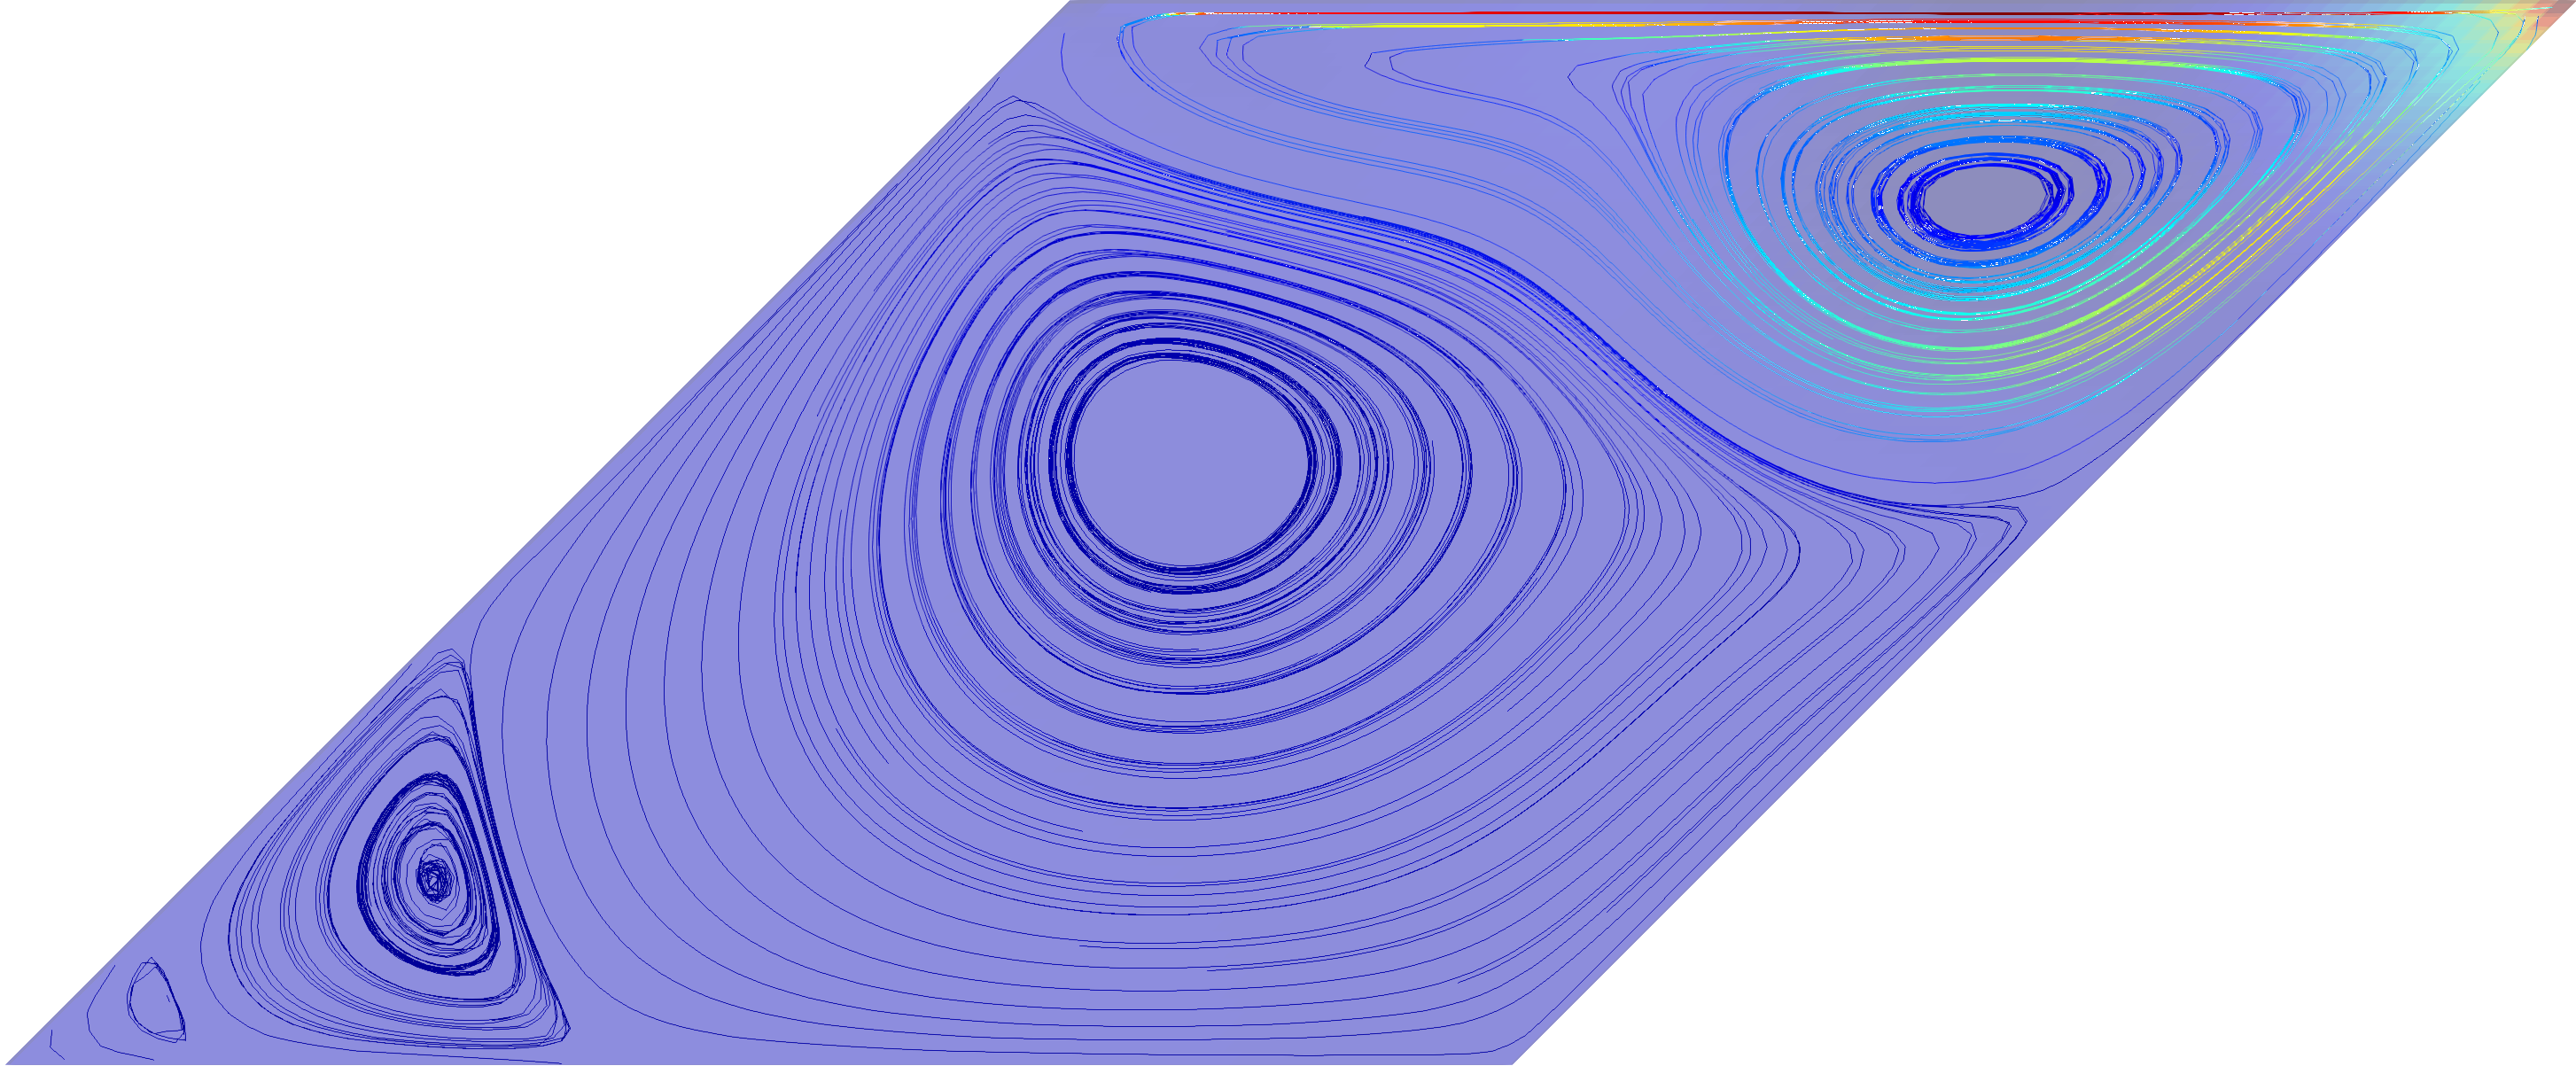
\includegraphics[width=1.055\textwidth]{pics/StreamlinesAtPressureCrop.png}};
            \draw (0,0,0)--(1,0,0)--(1.7071,0.7071,0.0)--(0.7071,0.7071,0.0)--cycle;
            \draw [color=black] (0.5,0,0)--(1.2071,0.7071,0);
            
            \draw [->,>=stealth](0.7071,0.735,0.0)-- (1.7071,0.735,0.0);
            \draw  (1.2071,0.72,0) node[above] {$\vec{U}_b$};
            
            \draw  (0.5,0,0) node[below] {$B$};
            \draw  (1.2071,0.7071,0) node[below] {$A$};

            \draw (0.15,0) arc (0:65:1mm);
            \draw (0.18,0.04,0) node[above] {$\alpha$};
        \end{tikzpicture}
        \caption{}
    \end{subfigure}
    \begin{subfigure}[b]{0.45\textwidth}
        \centering
        \begin{tikzpicture}[scale=4.5, every node/.style={scale=1}]
            \node[anchor=south west,inner sep=0] at (0,0) {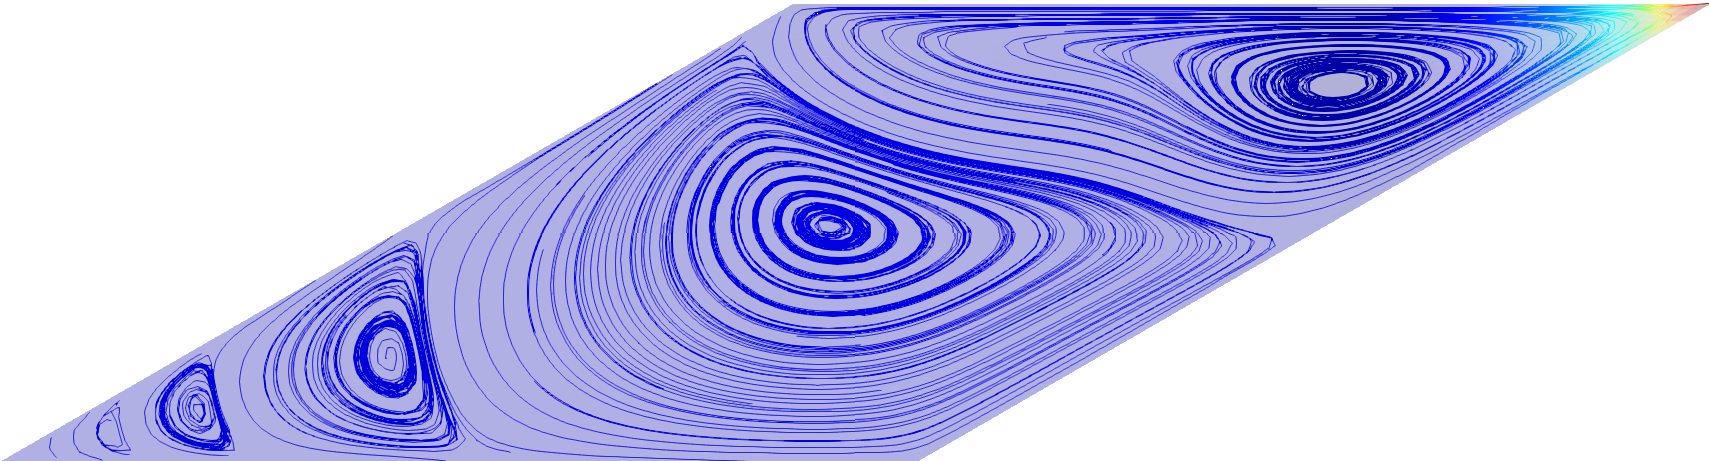
\includegraphics[width=1.15\textwidth]{pics/StreamlinesAtPressureCropTikz30.png}};
            \draw (0,0,0)--(1,0,0)--(1.86,0.5,0.0)--(0.86,0.5,0.0)--cycle;
            \draw [color=black] (0.5,0,0)--(1.36,0.5,0);
            
            \draw [->,>=stealth](0.86,0.523,0.0)-- (1.86,0.523,0.0);
            \draw  (1.35,0.52,0) node[above] {$\vec{U}_b$};
            
            \draw  (0.5,0,0) node[below] {$B$};
            \draw  (1.3071,0.5071,0) node[below] {$A$};

            \draw (0.21,0) arc (0:65:1mm);
            \draw (0.28,0.04,0) node[above] {$\alpha$};
            
        \end{tikzpicture}
        \caption{}
    \end{subfigure}
    \caption{Схематичное представление верификационной задачи с косоугольной каверной, горизонтальная компонента скорости замеряется вдоль линии AB.}
    \label{fig:SCav}
\end{figure}

\paragraph{Обратный уступ}

Для моделирования вязкой жидкости, алгоритму необходимо быть чувствительным к изменению числа Рейнольдса. Задача обратного уступа это простой и эффективный способ проверить эту чувствительность. На вход в расчетную область подается параболический профиль скорости. Все стенки кроме входа и выхода подчиняются условию прилипания для скорости и нулевого градиента для давления. 

После стабилизации потока измеряется расстояния от левой твердой стенки до точки разворота потока($d$) (см рис. \ref{fig:backwardStepSketch}). Полученное значение $d$ сравнивается с эталонным из \cite{ElizarBook}. Результаты показывают что QHDFoam корректно разрешает вязкие течения (см. рис. \ref{StreamRe100})

\begin{figure}[!h]
    \centering
    \begin{tikzpicture}[scale=1.5, every node/.style={scale=1}]
        \draw[thick] (0,2,0)--(0,1,0)--(1.0,1.0,0.0)--(1.0,0.0,0.0)--(8.0,0.0,0.0)--(8.0,2.0,0.0)--cycle;
            
        \draw (0.0,1.0) arc(-90:90:1cm and 0.5cm);
        \draw [->,>=stealth](0.0,1.5,0.0)-- (1,1.5,0.0);
        \draw [->,>=stealth](0.0,1.25,0.0)-- (0.8,1.25,0.0);
        \draw [->,>=stealth](0.0,1.75,0.0)-- (0.8,1.75,0.0);
        
        
        \draw (2.06,0.06) arc(-90:270:1cm and 0.4cm);
        \draw [<->,>=stealth](1,-0.1)--(5.2,-0.1);
        \draw (3,0.0,0) node[below] {$d$};
        
        \draw [<->,>=stealth](-0.1,1)--(-0.1,2);
        \draw (-0.1,1.5,0) node[left] {$h$};
        
        \draw [<->,>=stealth](7.7,0)--(7.7,2);
        \draw (7.7,1,0) node[left] {$2 \cdot h$};
        \draw (1.0,1.0) arc(90:53.5:7cm and 5cm);
    \end{tikzpicture}
    \caption{Схематичное изображение задачи с обратным уступом.}
    \label{fig:backwardStepSketch}
\end{figure}

\begin{figure}[!h]
    \centering
    \begin{subfigure}{\textwidth}
        \centering
        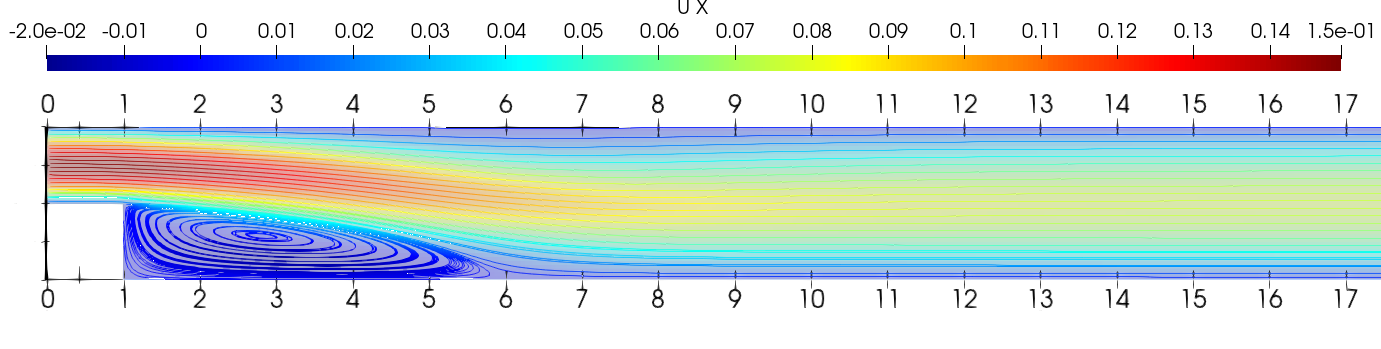
\includegraphics[scale=0.4]{pics/Re100.png}
        \caption{Re=100}
    \end{subfigure}
    \begin{subfigure}{\textwidth}
        \centering
        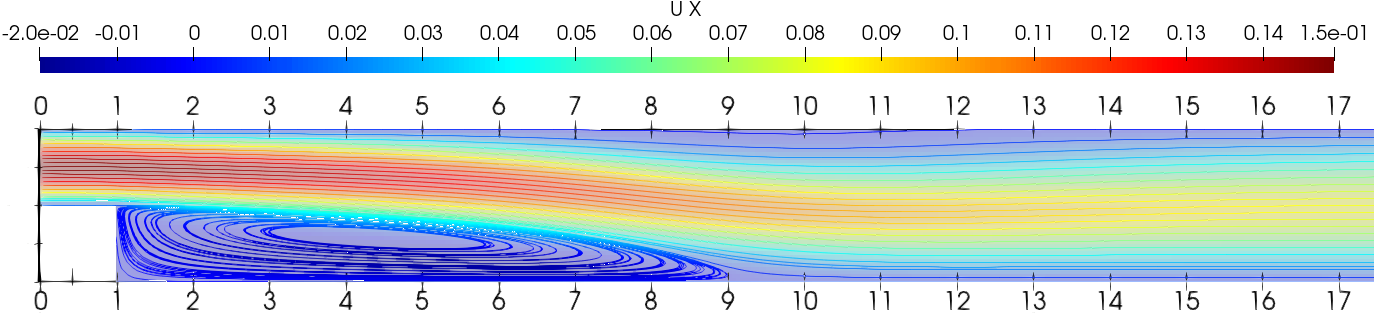
\includegraphics[scale=0.4]{pics/Re200.png}
        \caption{Re=200}
    \end{subfigure}
    \begin{subfigure}{\textwidth}
        \centering
        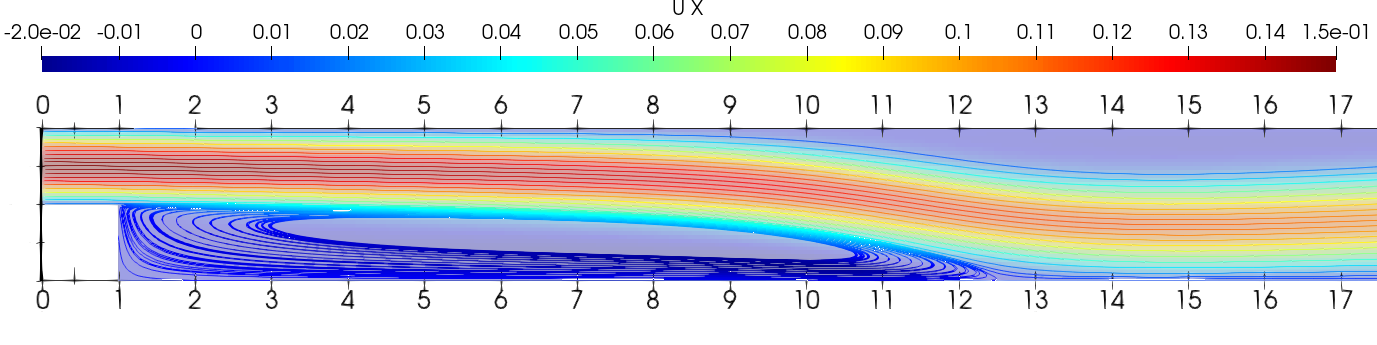
\includegraphics[scale=0.4]{pics/Re400.png}
        \caption{Re=400}
    \end{subfigure}
    \caption{Линии тока для задачи с обратным уступом}
    \label{StreamRe100}
\end{figure}


\begin{table}[!hb]
\caption {Сравнение результатов для задачи обратного уступа}
\noindent\begin{tabular}{l|ccc}
Research & $Re=100$ & $Re=200$  & $Re=400$ \\
\hline
QHDFoam & 5.0 & 8.25 & 11.9\\
Sparrow E. M. and Chuck W.\cite{Sparrow1987} & 5.0 & 7.5 & -\\
Kim J. and Moin P.\cite{Kim1985} & 5.0 & 8.3 & 12 \\
Hackman L. P. et al.\cite{Hackman1984} & 5.0 & 8.5 & -\\
\hline
Armaly B. F. et al.\cite{Armaly1983} & 5.0 & 8.5 & 14.2
\end{tabular}
\label{table:tabBackward}
\end{table}

\paragraph{Естественная конвекция}

Рассматривается задача естественной конвекции в каверне согласно \cite{ElizarBook} значение регуляризационного параметра было вычислено пропорционально обратному числу Грастгофа $Gr^{-1}$, которое было порядка $10^{-4}$ с. Сравнение максимумов горизонтальной и вертикальной скорости с данными из \cite{ElizarBook} и \cite{Vabishevich} показывают сеточную сходимость и хорошую согласованность между QHDFoam и рассматриваемыми в работах методами. Результаты сравнения видны в таблице \ref{table:tabHotCavityHor} . Линии тока изображены на рисунке \ref{fig:Nconv}. Схему расчетной области можно увидеть на рисунке \ref{fig:convectionScratch}

\begin{table}[!hb]
\caption { Сравнение максимума горизонтальной компоненты скорости для задачи естественной конвекции.}
\centering
\noindent\begin{tabular}{l|ccc}
Mesh & $U_x$ \cite{ElizarBook} & $U_x$ \cite{Vabishevich} & $U_x$ \textit{QHDFoam} \\
\hline
$20\times20$ & 15.938 & 16.144 & 16.040\\
$40\times40$ & 16.005 & 16.262 & 16.410\\
$80\times80$ & 16.070 & 16.219 & 16.225
\end{tabular}
\label{table:tabHotCavityHor}
\end{table}

 \begin{table}[!h]
\centering
\caption {Сравнение максимума вертикальной компоненты скорости для задачи естественной конвекции.}
\noindent\begin{tabular}{l|ccc}
Mesh & $U_y$ \cite{ElizarBook} & $U_y$ \cite{Vabishevich} & $U_y$ \textit{mulesQHDFoam} \\
\hline
$20\times20$ & 19.513 & 19.363 & 19.670\\
$40\times40$ & 19.663 & 19.602 & 19.910\\
$80\times80$ & 19.663 & 19.648 & 19.757
\end{tabular}
\label{table:tabHotCavityVer}
\end{table}

\begin{figure}
    \centering
    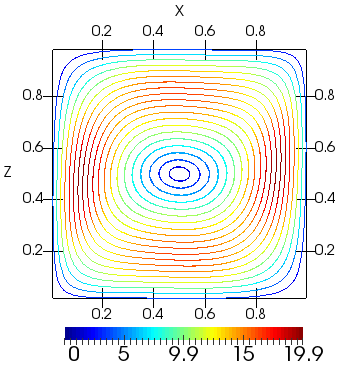
\includegraphics[scale=0.9]{pics/Umag.png}
    \caption{Линии тока для задачи естественной конвекции}
    \label{fig:Nconv}
\end{figure}

\begin{figure}
    \centering
    \begin{tikzpicture}[scale = 8]
        \draw[thick] (0,0,0) -- (1,0,0) -- (1,1,0) -- (0,1,0) -- cycle;
        
        \draw[thick, color = red] (0,0,0) -- (0,1,0);
        
        \draw[thick, color = blue] (1,0,0) -- (1,1,0);
        \draw (0.95,0.75) node[left,rotate=90] {$T=0^{\circ}$};
        
        \draw [<->,>=stealth](-0.025,0)--(-0.025,1);
        \draw (-0.075,0.9) node[left,rotate=90] {$L=1 m,$  $T=1^{\circ}$};
        
        \draw [<->,>=stealth](0,1.025)--(1,1.025);
        \draw (0.5,1.025) node[above] {$L=1 m$};
        \draw[ very thick,->, >=stealth] (0.15,0.9)  ++ (-50:.75) arc (300:-50:.25 and .25);
        
    \end{tikzpicture}
    \caption{Схематичное изображение задачи для естественной конвекции}
    \label{fig:convectionScratch}
\end{figure}

\subsection{Валидация}

Аттрактор внутренних волн -- это сложное явление, которое происходит после многократного отражения внутренних волн от стенок резервуара. PISO алгоритмы из предыдущего раздела не справляются с моделированием этого феномена, но результаты моделирования аттрактора с помощью решателя QHDFoam показывают неплохие результаты. Удалось добиться ошибки меньше 3\% см. Рис. \ref{fig:AdamsBashforthEulerNek3D}.

\begin{figure}[hbt!]
    \centering
        
    \begin{tikzpicture}[scale = 1,spy using outlines={circle, magnification=6, connect spies}]
        \begin{axis}
            [scale only axis, xlabel=Линия пробы $m \cdot 10^{-3}$, ylabel=$U_x\;\; m/s \cdot 10^{-3}$, grid=major,legend style={at={(0,1),font=\LARGE},anchor=north west}, ymin=-0.8, ymax=0.8,xmin=0,xmax=20,legend style={nodes={scale=0.5, transform shape}}, x post scale=1.6]

            \addplot[solid,color=black,thick] table [x=Points:1, y=U, col sep=comma] {CSV/NEK5000.csv};
            \addplot[solid,color=red,thick] table [x=Points:1, y=U, col sep=comma] {CSV/QHD480x320.csv};
            \addplot[solid,color=green!60!black,thick] table [x=Points:1, y=U, col sep=comma] {CSV/QHD240x160.csv};
            \addplot[solid,color=blue,thick] table [x=Points:1, y=U, col sep=comma] {CSV/QHD240x1602tau.csv};
            \legend{NEK500,QHDFoam 480x320, QHDFoam 240x160, QHDFoam 240x160 $\tau \cdot 2$}

            \coordinate (spypoint) at (axis cs:14.7,0.7);
            \coordinate (magnifyglass) at (axis cs:15.5,-0.3);
        \end{axis}
        \spy [blue, size=4cm] on (spypoint) in node[fill=white] at (magnifyglass);
    \end{tikzpicture} 
    \caption{Количественное сравнение результатов моделирования}
    \label{fig:AdamsBashforthEulerNek3D}
\end{figure}


Также количественные исследования демонстрируют сходимость решения получаемое с помощью квазигидродинамических уравнений к решению полученному с помощью метода высокого порядка (см. Рис. \ref{fig:tauAttr}) в отличие от результатов полученных с помощью PISO (см. Рис. \ref{fig:PISOattr}).

\begin{figure}
    \centering
        \begin{tikzpicture}[scale = 1.1]
          \begin{axis}
             [scale only axis, grid=major,legend style={at={(0,1),font=\LARGE},anchor=north west}, ymin=-0.8*10^-3, ymax=1.7*10^-3, xmin=0.0,legend style={nodes={scale=0.5, transform shape}}, x post scale=1.5,xlabel={$y$}, ylabel={$U_x$}];
            \addplot[solid,color=red,thick] table [x=Points:1, y=U:0, col sep=comma] {CSV/Ux300.5tau.csv};
            \addplot[solid,color=green,thick] table [x=Points:1, y=-U:0, col sep=comma] {CSV/Ux301tau.csv};
            \addplot[solid,color=blue,thick] table [x=Points:1, y=U:0, col sep=comma] {CSV/Ux302tau.csv};
            %\addplot[solid,color=violet,dashed,thick] table [x=Points:1, y=-U:0, col sep=comma] {CSV/Ux30tau001200sBackward.csv};
            \legend{$\tau = 0.005$,$\tau = 0.01$,$\tau = 0.02$,Adams-Bashforth}
          \end{axis}
          \begin{axis}
            [scale only axis, ymin=-0.8*10^-1, ymax=1.7*10^-1, xmin=0.0,  yticklabels={,,},xticklabels={,,},legend style={at={(0,0.75),font=\LARGE},anchor=north west},legend style={nodes={scale=0.5, transform shape}},x post scale=1.5];
            \addplot[solid,thick] table [x=Points:1, y=x_velocity, col sep=comma] {CSV/Ux30Nek500T200.csv};
            \legend{NEK5000}
          \end{axis}
        \end{tikzpicture} 
    \caption{Распределение скорости вдоль линии AB. Демонстрируется сходимость по $\tau$.}
    \label{fig:tauAttr}
\end{figure}

Помимо точности реализаций алгоритмов на базе пакета OpenFOAM сравнивалась и скорость их работы на 12 ядрах процессоров Intel X5670 (Таб. \ref{tab:perfom}). Наиболее быстрый метод– метод спектральных элементов. Для того чтобы достичь отметки в 100 с модельного времени потребовалось время исполнение чуть больше тысячи секунд. Сравнение с методом спектральных элементов является условным из-за значительных отличий в реализации. Один спектральный элемент состоит из 81 точки интерполяции, поэтому количество спектральных элементов настолько мало. PISO алгоритм отстал от алгоритма на базе квазигидродинамического подхода более чем в полтора раза при одинаковых условиях расчёта. Такое отставание и объясняется наличием коррекционных циклов, которые отсутствуют в квазигидродинамическом подходе. 

\begin{table}[]
    \caption{\label{tab:perfom}Сравнение производительности на процессоре Intel(R) Xeon(R) CPU X5670 2.93 GHz, 100 с модельного времени, с шагом в $5 \cdot 10^{-3}$, опции компиляции -- gcc -O3.}
    
    \begin{tabular}{c|c|c|c|c|c}
        Подход & Время  & Количество  & PIMPLE      & Коррекции  \\
                 & исполнения (с)   &   элементов  & коррекции & неортогональности     \\
        \hline
         &  & 1296 &  &  \\
        Nek5000 & 1037 & Спектральных & 0 & 0 \\
         &  & элементов &  &  \\
        \hline
         &  & 67 500 &  & \\
        PISO & 7630 & Конечных & 3 & 1\\
         &  & элементов &  & \\
        \hline
         &  & 67 500 &  & \\
        QHD & 4479 &  Конечных & 0 & 0\\
         &  & элементов &  & \\
        \hline
    \end{tabular}
    
    \end{table}

\section*{Заключение к главе 2}

В этой главе рассмаотрены способы моделирования аттракторов внутренних волн. Первая часть посвящена обзору существующих коллективов, которые исследуют фокусировку внутренних волн в лабораторных условиях. В главе также описаны экспериментальные установки, которые используются этими коллективами. 

Также освещены методы численного моделирования аттракторов внутренних волн. Метод спектральных элементов очень мощный инструмент высокого порядка. Однако, метод спектральных элементов очень чувствителен к вычислительной сетке и геометрии. Этот метод не подходит для моделирования аттракторов внутренних волн в естественных условиях сложной топологии океанического дна или при наличии примесей описываемых частицами в воде.

Альтернативный метод -- метод конечных объемов. Позволяет проводить численные эксперименты в условиях приближенных к реальным, включая сложную геометрию океанического дна и осаждение примесей. Однако, его реализация на одной из самых популярных платформ не демонстрирует сеточной сходимости и количественного соответствия методу спектральных элементов. Поддерживаемом метод конечных объемов не позволяет достичь той точности, что гарантирует метод спектральных элементов. Стандартные средства популярных инструментов моделирования несжимаемых течений не могут количественно воспроизвести эффекты множественной фокусировки внутренних волн. 

Подход на основе квазигидродинамических уравнений имеет простой вычислительный алгоритм, количественное совпадение результатов с результатами полученными при помощи метода спектральных элементов.

В этой главе рассмотрены аспекты реализации квазигидродинамического подхода, верификации разработанного алгоритма и валидации на примере задачи формирования аттрактора внутренних волн сравниваются результаты работы алгоритма PISO и QHD. Результаты количественно сравнивались с эталонным решением, полученным при помощи метода спектральных элементов.

Анализ полученных результатов позволяет сделать следующие выводы:
\begin{itemize}
    \item На верификационной задаче о моделировании стационарного течения в скошенной каверне оба метода ведут себя одинаково адекватно, наблюдается сеточная сходимость численных результатов, что говорит об устойчивости методов на деформированных сетках.
    \item На задаче о моделировании формирования аттрактора гравитационных внутренних волн QHD алгоритм показывает результаты как количественно, так и качественно воспроизводящие это явление, как на малых, так и на больших временах. Алгоритм PISO воспроизводит явление лишь качественно и только на небольших временах.
    \item QHD алгоритм показывает сеточную сходимость и сходимость по регуляризационному настроечному параметру. PISO алгоритм не демонстрирует сеточной сходимости при сгущении пространственной сетки.
    \item QHD алгоритм, построенный на базе квазигидродинамических уравнений, не требует дополнительных коррекций вычисленных скоростей и давлений в отличие от алгоритма PISO.
    \item OpenFOAM реализация квазигидродинамического подхода показала более высокую производительность на многопроцессорной системе чем реализация алгоритма PISO.
\end{itemize}

Исходя из вышесказанного можно констатировать преимущества алгоритма QHD при моделировании аттракторов внутренних волн по сравнению со стандартными средствами, ранее реализованными в OpenFOAM на базе алгоритма PISO. 


%
%\backmatter %% Здесь заканчивается нумерованная часть документа и начинаются ссылки и
%            %% заключение
\chapter{Волновые движения в замкнутом резервуаре при воздействии с двумя частотами}



Известно, что в океане существует великое множество волн. Вопрос будут ли волны различных частот мешать образовываться аттрактору до сих пор остается открытым. В данной работе изучается вопрос совместного воздействия на стратифицированную жидкость волнопродуктора с двумя различными частотами и одинаковой амплитудой. 

Постановка задачи несколько меняется. Для моделирования используется конфигурация представленная на рисунке \ref{fig:domainup}. Условие на волнопродукторе будет теперь записываться следующим образом:

\begin{equation}
    U_z = A_1\cdot cos\left(\frac{\pi \cdot z}{L_1}\right)\cdot \omega_1 \cdot  sin(\omega_1 t) + A_2\cdot cos\left(\frac{\pi \cdot z}{L_1}\right)\cdot \omega_2 \cdot  sin(\omega_2 t)
\end{equation}

Посчитаны различные режимы:

\begin{itemize}
    \item Режим разнесенными частотами, $\omega_1/N=0.58$ $\omega_2/N=0.66$ и малой амплитудой $a=0.02$ см. 
    \item Режим с совпадающими частотами, $\omega_1=\omega_2=0.628$ и амплитудой $a=0.05$ см.
    \item Режим с приближенными частотами, $\omega_1/N=0.66$ $\omega_2/N=0.68$ и амплитудой $a=0.05$ см.
    \item Режим с близкими частотами $\omega_1/N=0.628$ $\omega_2/N=0.641$ и  амплитудой $a=0.05$ см.
\end{itemize}

Первый режим демонстрирует общую картину течения при взаимодействии с двумя частотами. На рисунке \ref{fig:biharmVyamp02} показано, что в одном резервуаре допустимо существования сразу двух аттракторов внутренних волн. Это видно по характерному распределению поля скоростей и давлений в резервуаре. В середине первого(том что соединяет нижнюю и наклонную стенку) луче аттрактора помещена точка пробы. Видно, что существует задержка между частотой колебания волнопродуктора и частотой колебаний в середине первого луча аттрактора. Помимо этого, построен спектр частот колебаний скорости, частоты на этом графике осреднены по большей из частот. Сама точка пробы также размещена на первом луче аттрактора, который возникает под воздействием большей из частот. Это объясняет то почему второй пик меньше. На протяжении всей частотно-временной диаграммы наблюдается доминация этих двух частот.

\begin{figure}
  \centering
    \begin{subfigure}[с]{0.45\textwidth}
        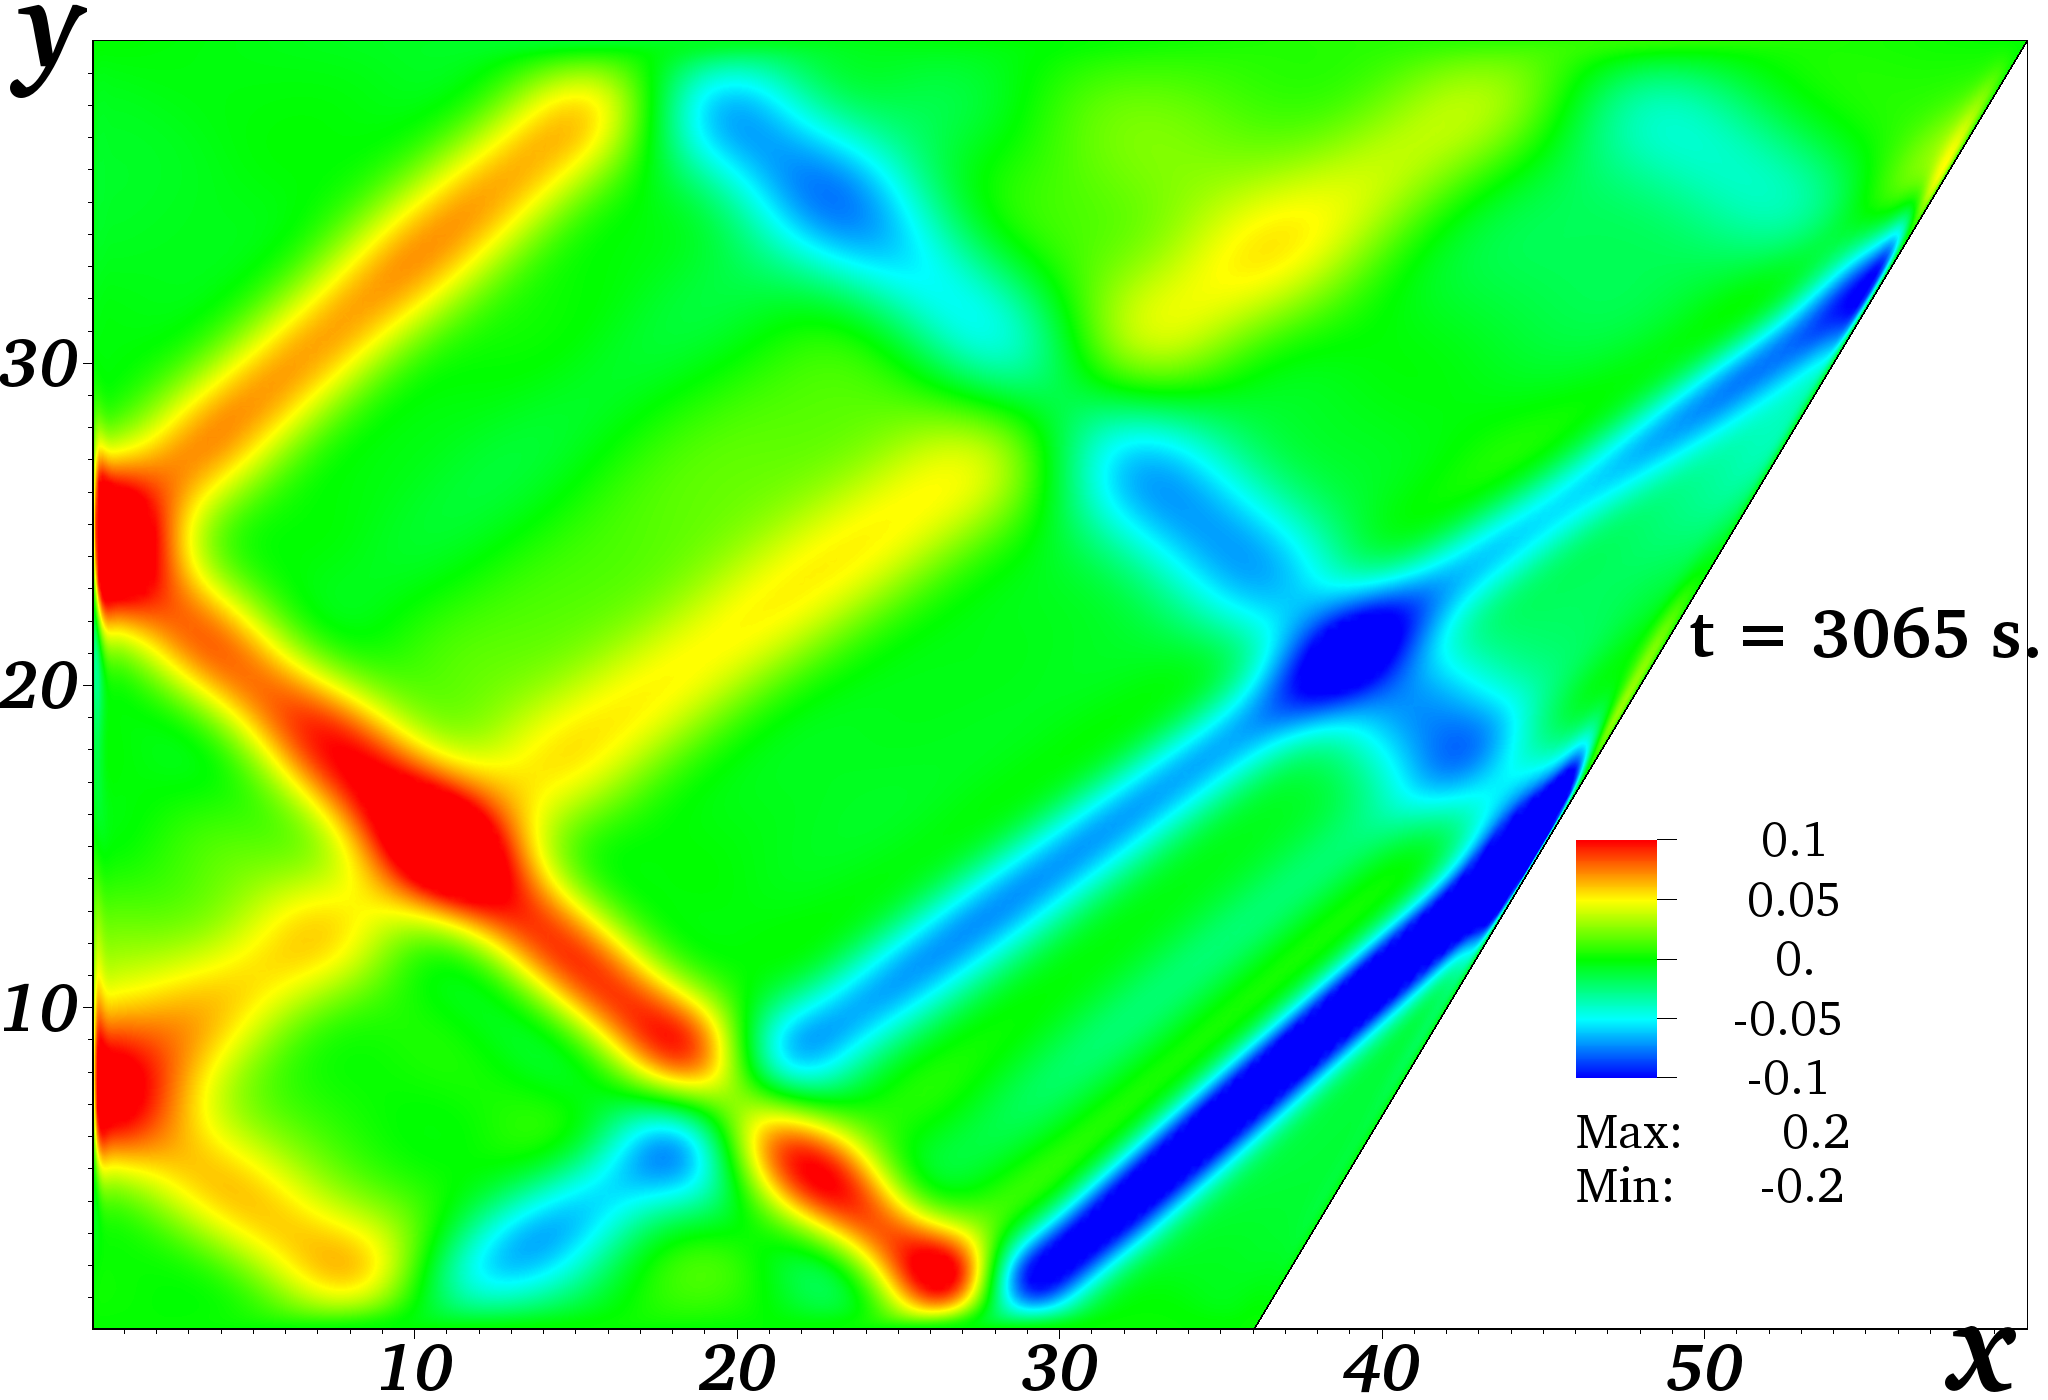
\includegraphics[width=1\textwidth]{pics/H40L60N1ap02dp20w1p58w2p66Biharm/2D36x36DiagramH40L60N1ap02dp20w1p58w2p66BiharmVyn06129.png}
        \caption{Вертикальная компонента скорости}
    \end{subfigure}
    \begin{subfigure}[с]{0.45\textwidth}
        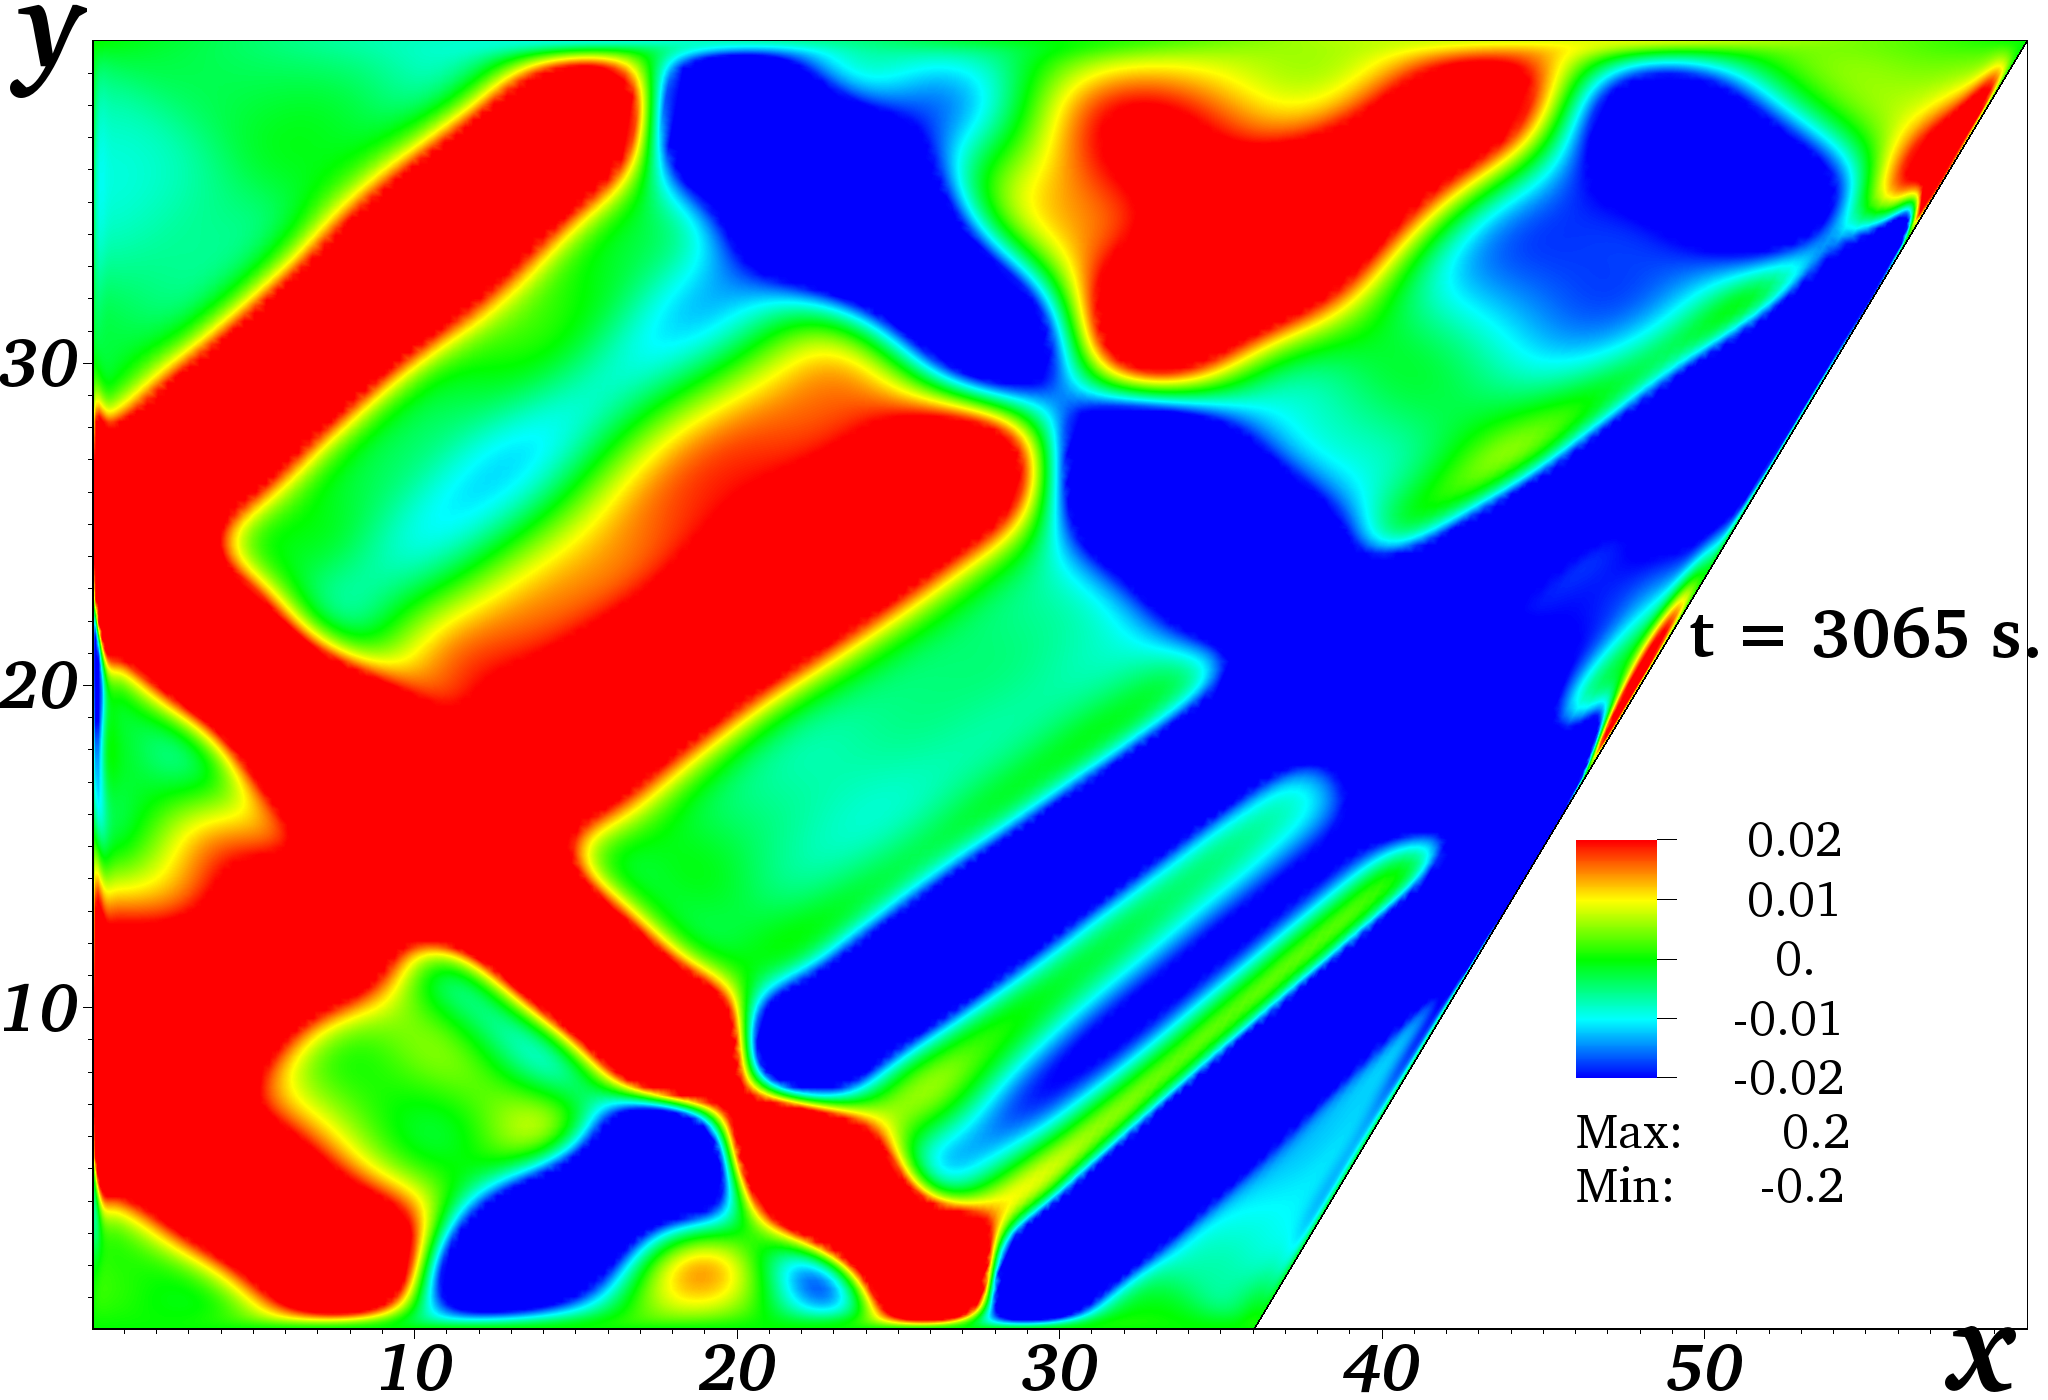
\includegraphics[width=1\textwidth]{pics/H40L60N1ap02dp20w1p58w2p66Biharm/2D36x36DiagramH40L60N1ap02dp20w1p58w2p66BiharmVy6129.png}
        \caption{Поле давления}
    \end{subfigure}
    \par
    \begin{subfigure}[с]{0.45\textwidth}
        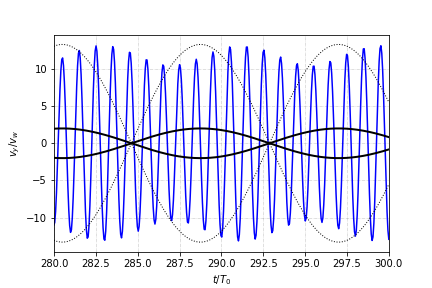
\includegraphics[width=1\textwidth]{pics/H40L60N1ap02dp20w1p58w2p66Biharm/vyX36p49Y7p94frm280to300.png}
        \caption{Вертикальная компонента скорости в середине первого луча аттрактора}
    \end{subfigure}
    \begin{subfigure}[с]{0.45\textwidth}
        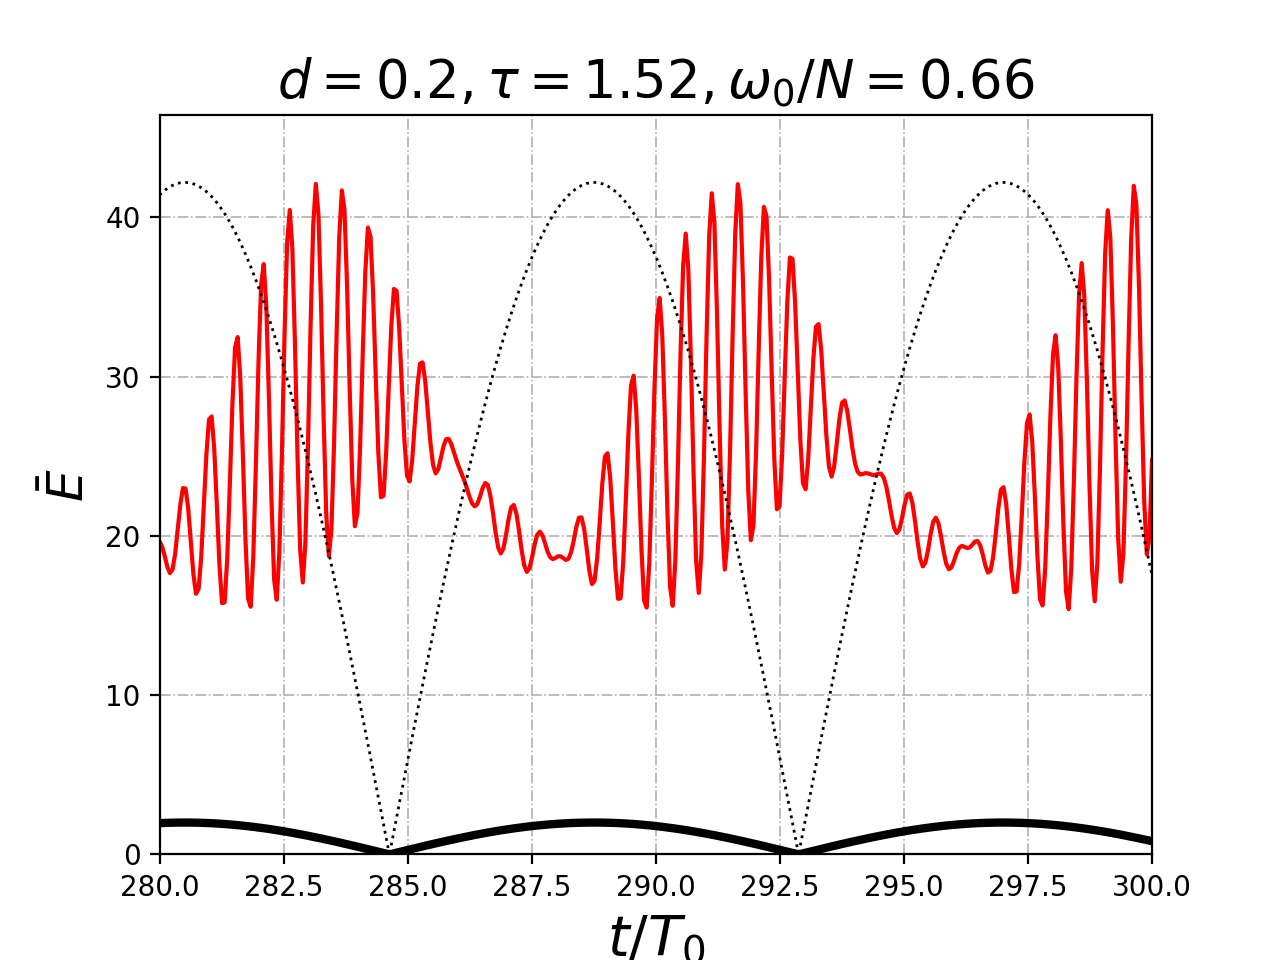
\includegraphics[width=1\textwidth]{pics/H40L60N1ap02dp20w1p58w2p66Biharm/2D36x36DiagramH40L60N1ap02dp20w1p58w2p66BiharmtotKEnonDim.png}
        \caption{Средняя кинетическая энергия в резервуаре}
    \end{subfigure}
    \par
    \begin{subfigure}[с]{0.45\textwidth}
        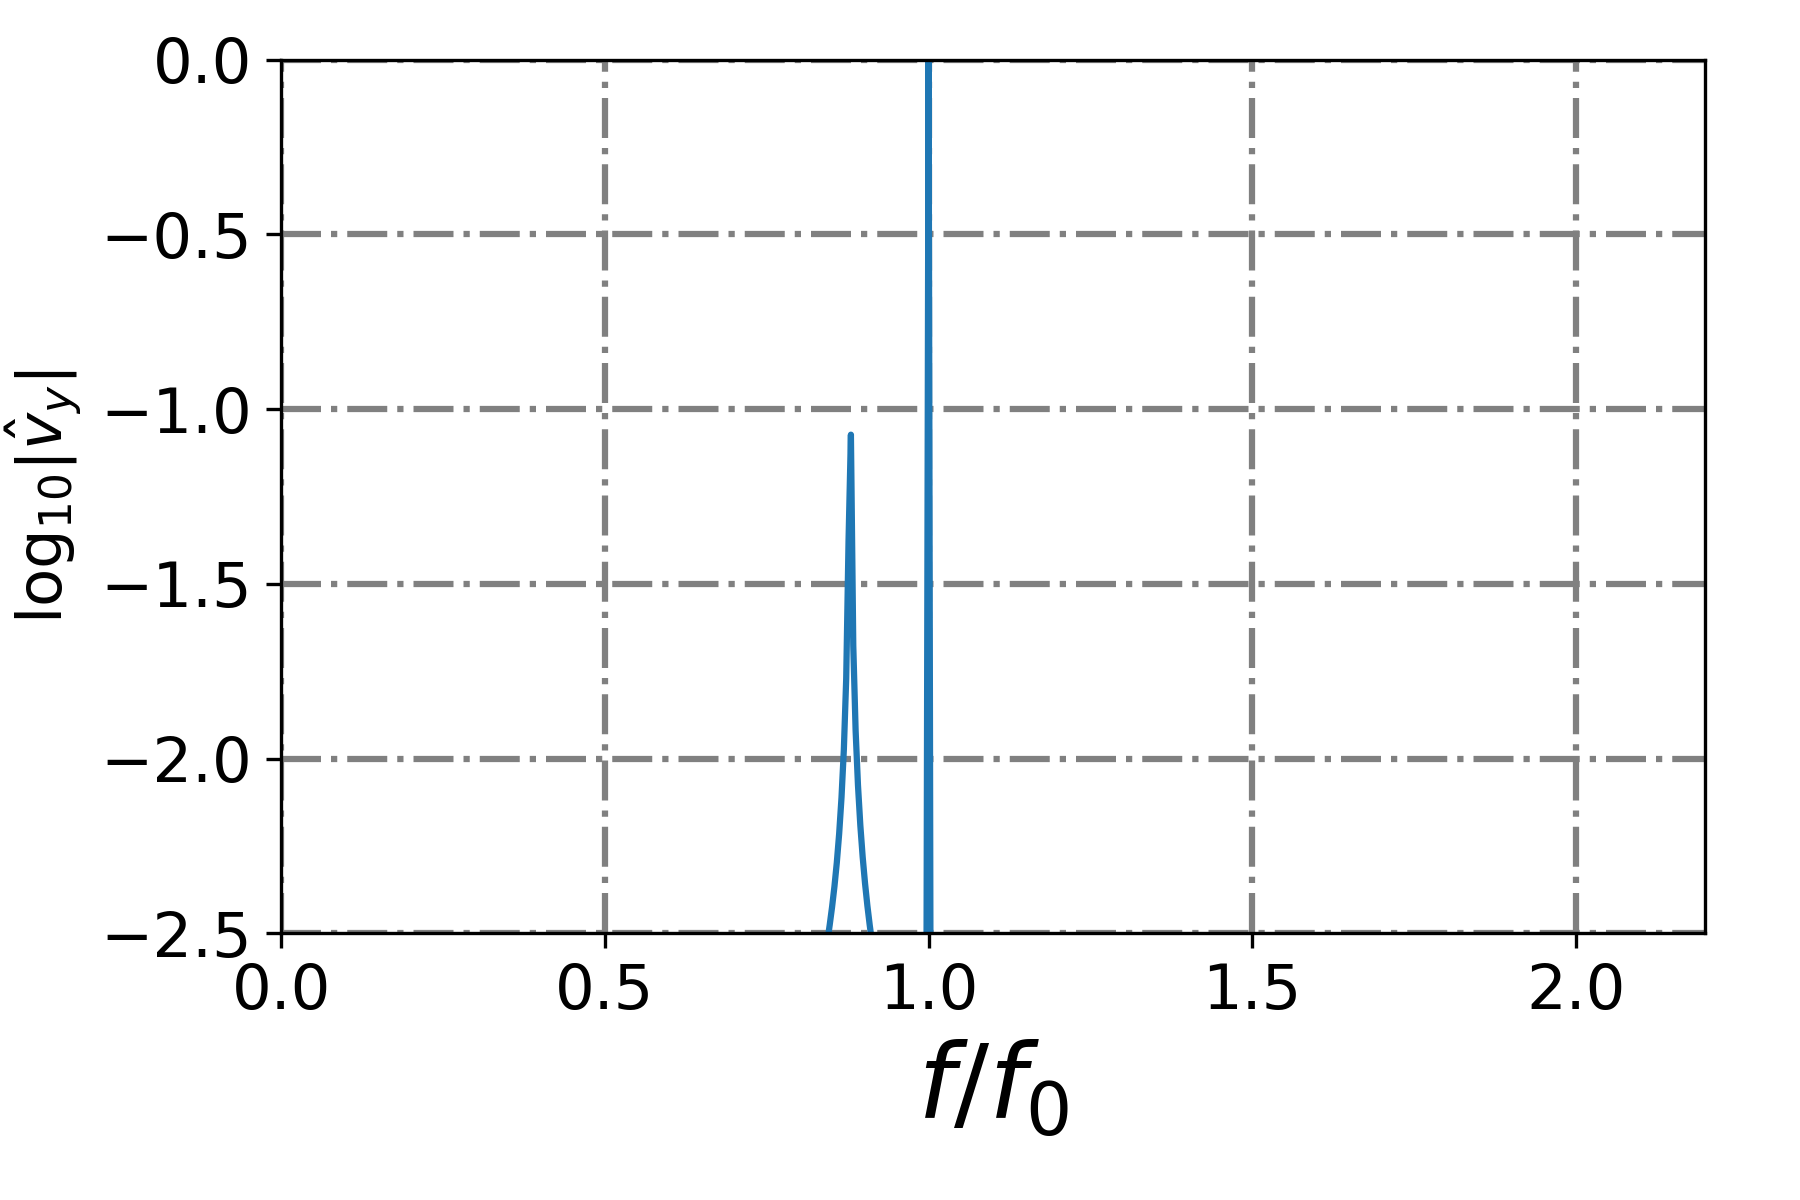
\includegraphics[width=1\textwidth]{pics/H40L60N1ap02dp20w1p58w2p66Biharm/spectrumX36p4Y8p0.png}
        \caption{Спектр}
    \end{subfigure}
    \begin{subfigure}[с]{0.45\textwidth}
        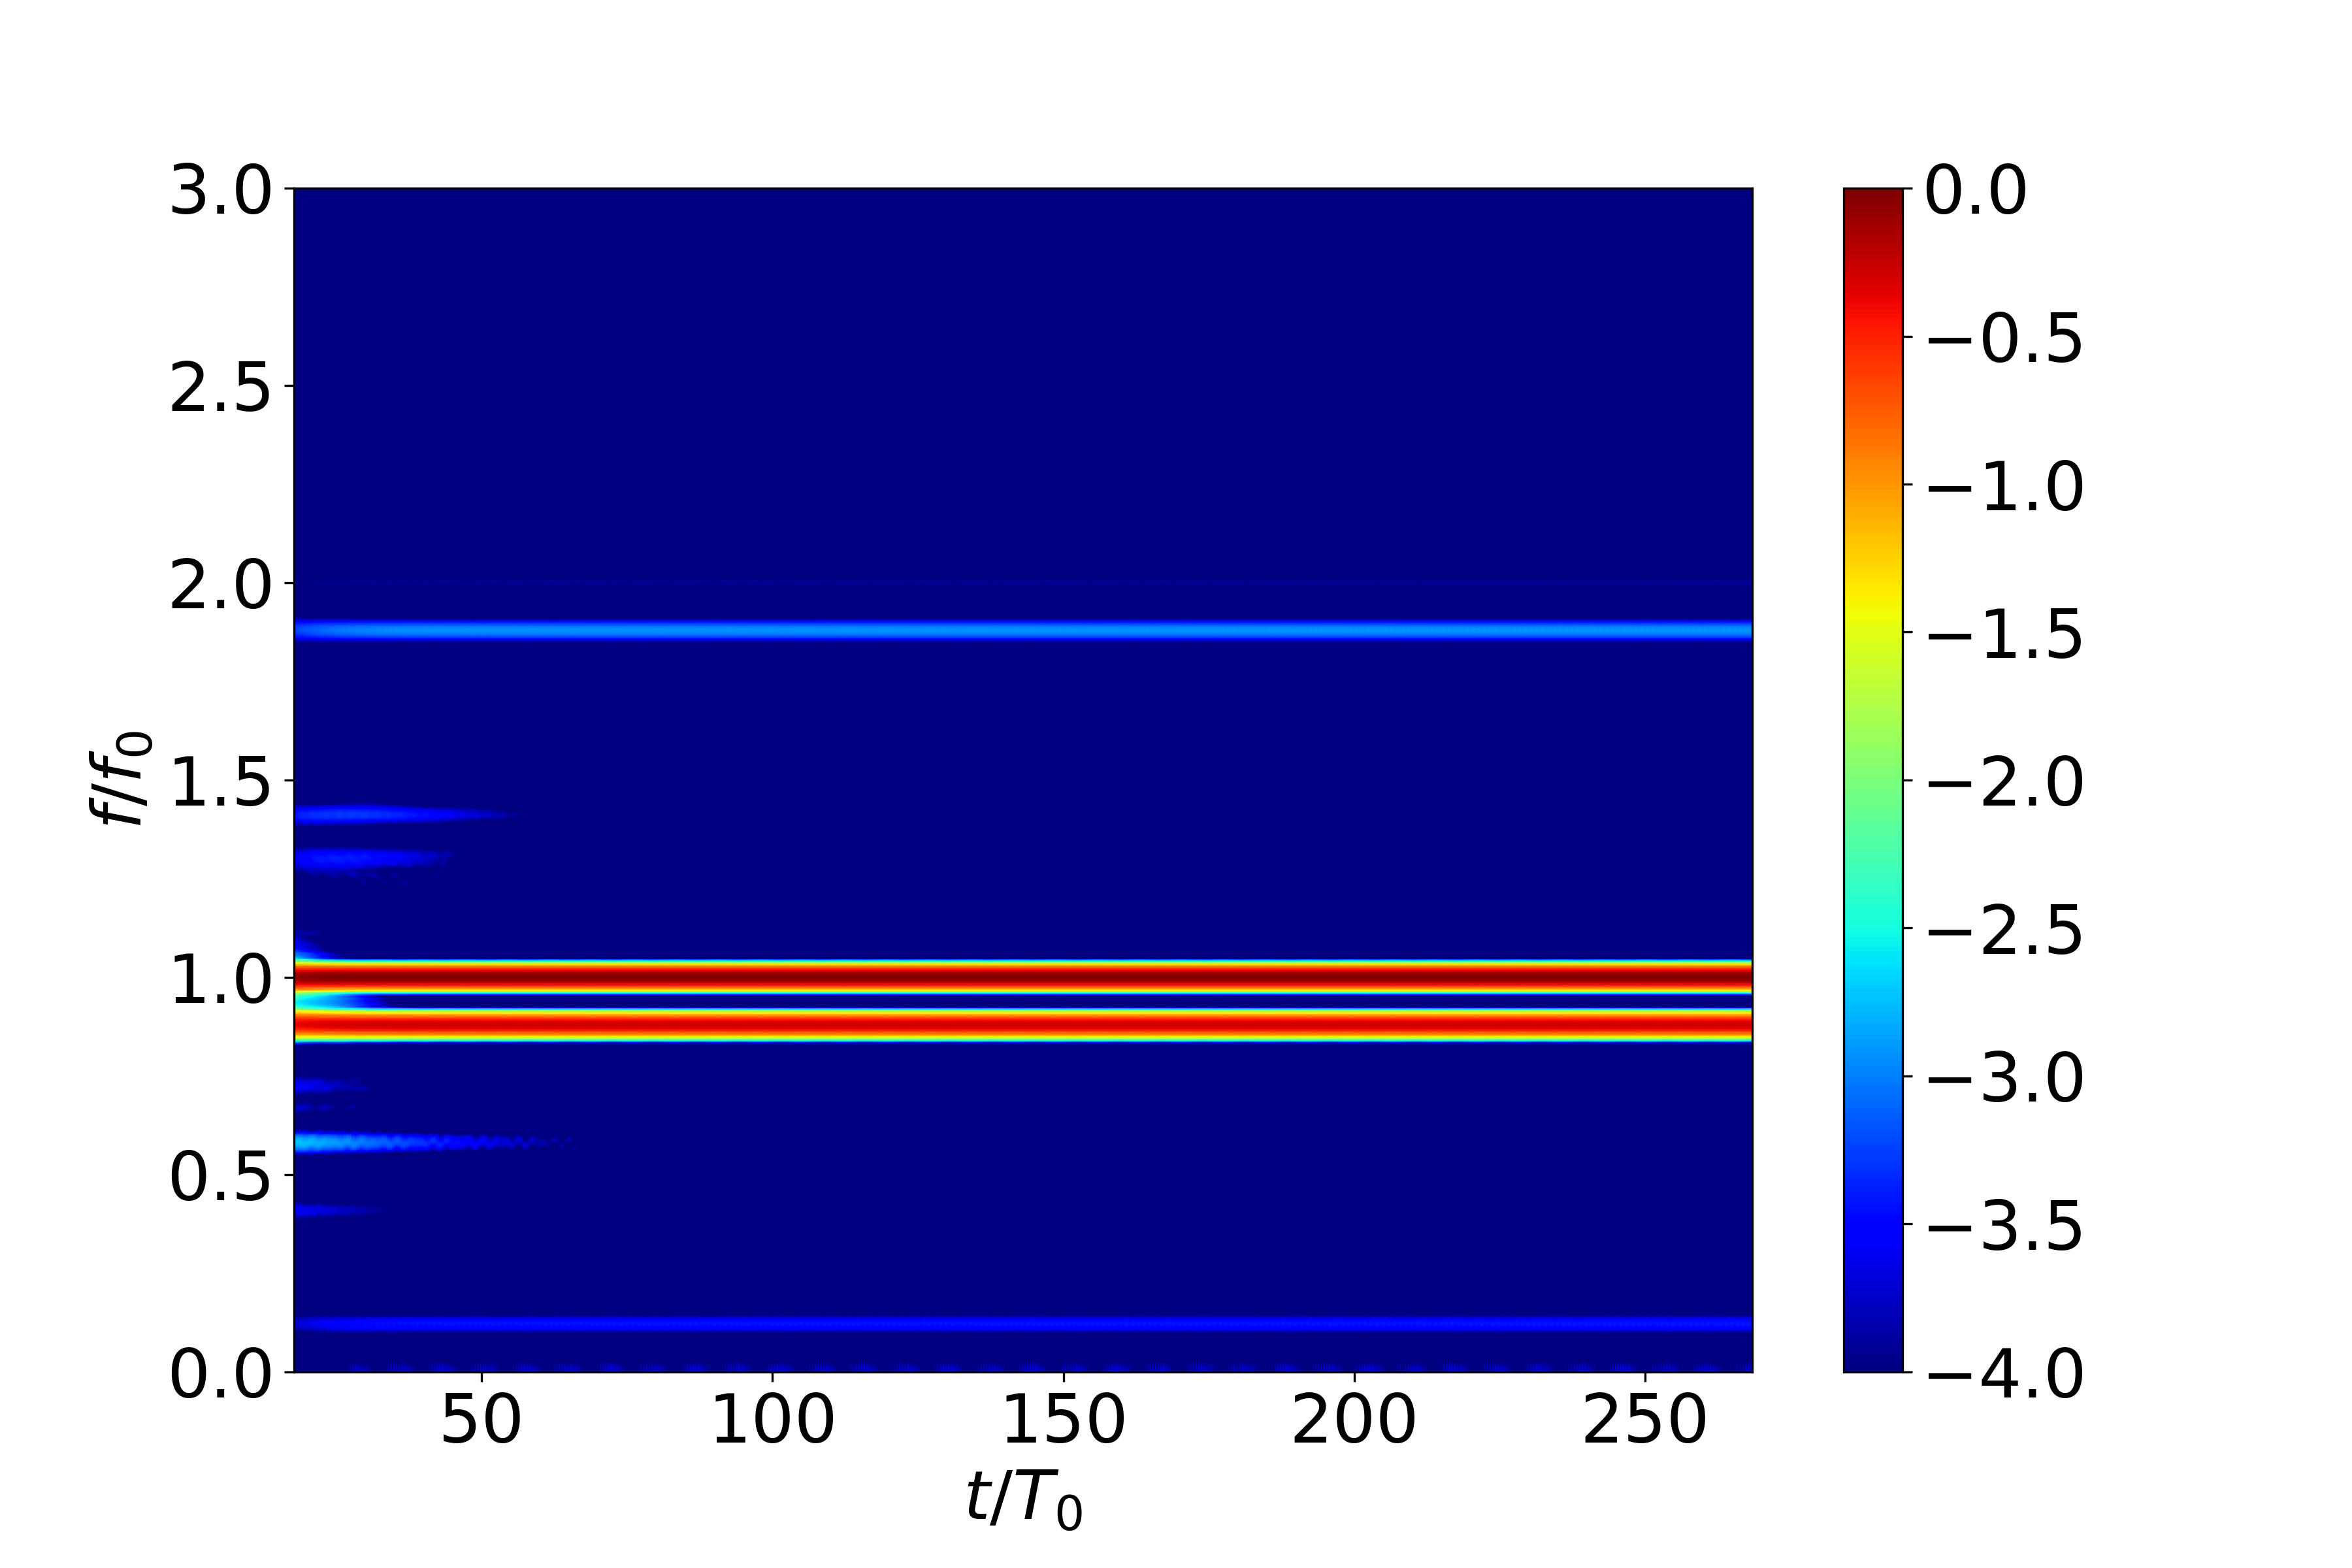
\includegraphics[width=1\textwidth]{pics/H40L60N1ap02dp20w1p58w2p66Biharm/TFspectrumX36p4Y8p0N768.png}
        \caption{Частотно-временная диаграмма}
    \end{subfigure}
    \caption{Результаты количественного исследования характеристик течения стратифицированной жидкости в трапециевидном резервуаре при внешнем воздействии с двумя разнесенными частотами $\omega_1/N=0.58$,  $\omega_2/N=0.66$. Черной линией  на графиках вертикальной скорости и кинетической энергии показана огибающая амплитуды колебаний волнпородуктора.}
    \label{fig:biharmVyamp02}
\end{figure}

Совпадение частот означает, что амплитуда колебаний удваивается значение $a=0.05$ cm. При $a=0.1$ на рисунке \ref{fig:Vyamp1} наблюдается неустойчивость этот режим характеризуется россыпью частот на спектре и частотно-временной диаграмме.

\begin{figure}
	\centering
	\begin{subfigure}[с]{0.45\textwidth}
	    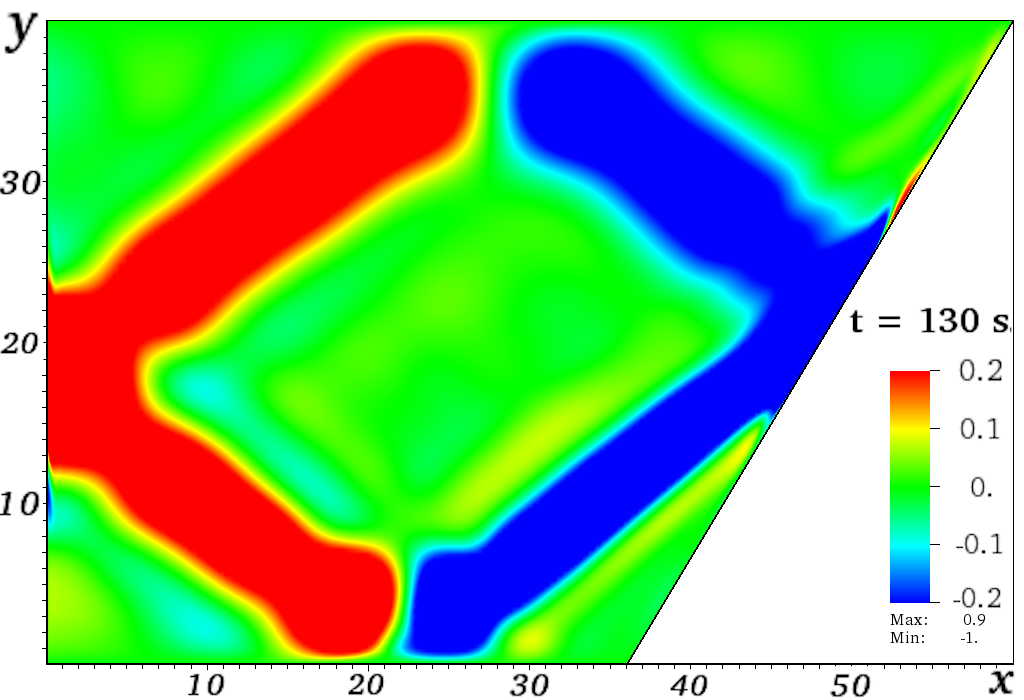
\includegraphics[width=1\textwidth]{pics/H40L60N1ap10dp20w0p63/2DH40L60N1ap10dp20w0p63Vyn00012.png}
	    \caption{Поле вертикальной скорости при образовании аттрактора}
	\end{subfigure}
	\begin{subfigure}[с]{0.45\textwidth}
	    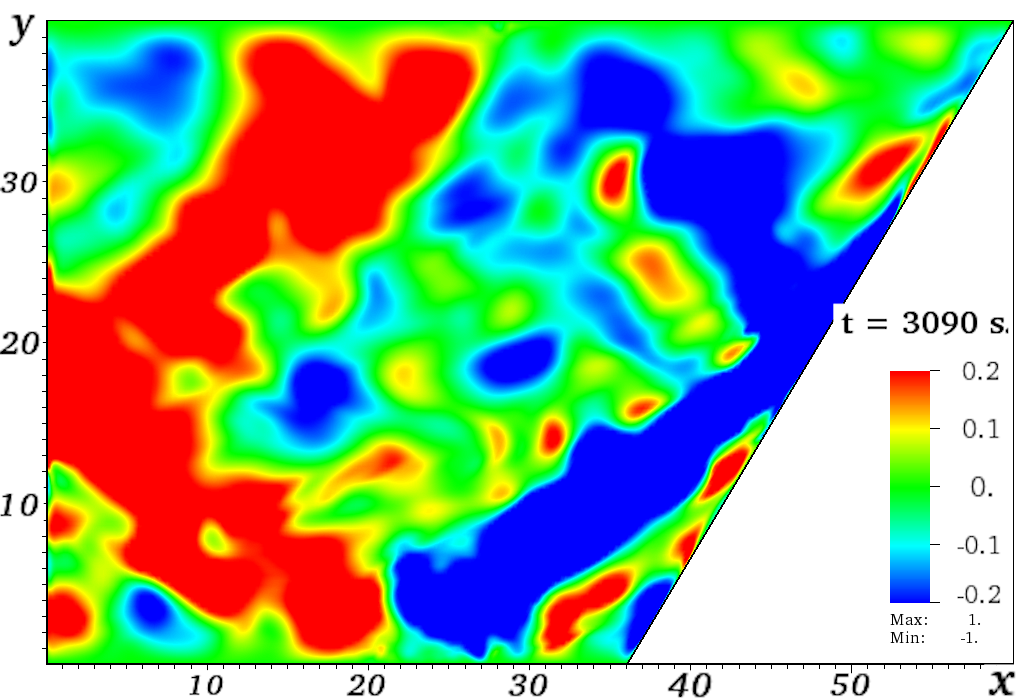
\includegraphics[width=1\textwidth]{pics/H40L60N1ap10dp20w0p63/2DH40L60N1ap10dp20w0p63Vyn00308.png}
	    \caption{Поле вертикальной скорости при образовании неустойчивостей}
	\end{subfigure}
	\par
	\begin{subfigure}[с]{0.45\textwidth}
	    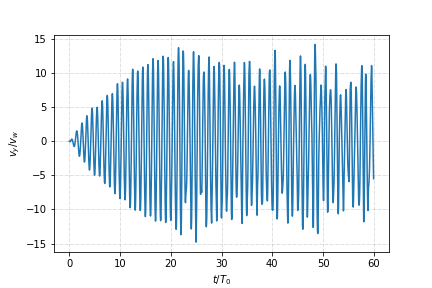
\includegraphics[width=1\textwidth]{pics/H40L60N1ap10dp20w0p63/vyX35p6Y11p3t1200.png}
	    \caption{зависимость скорости в середине первого луча аттрактора от времени}
	\end{subfigure}
	\begin{subfigure}[с]{0.45\textwidth}
	    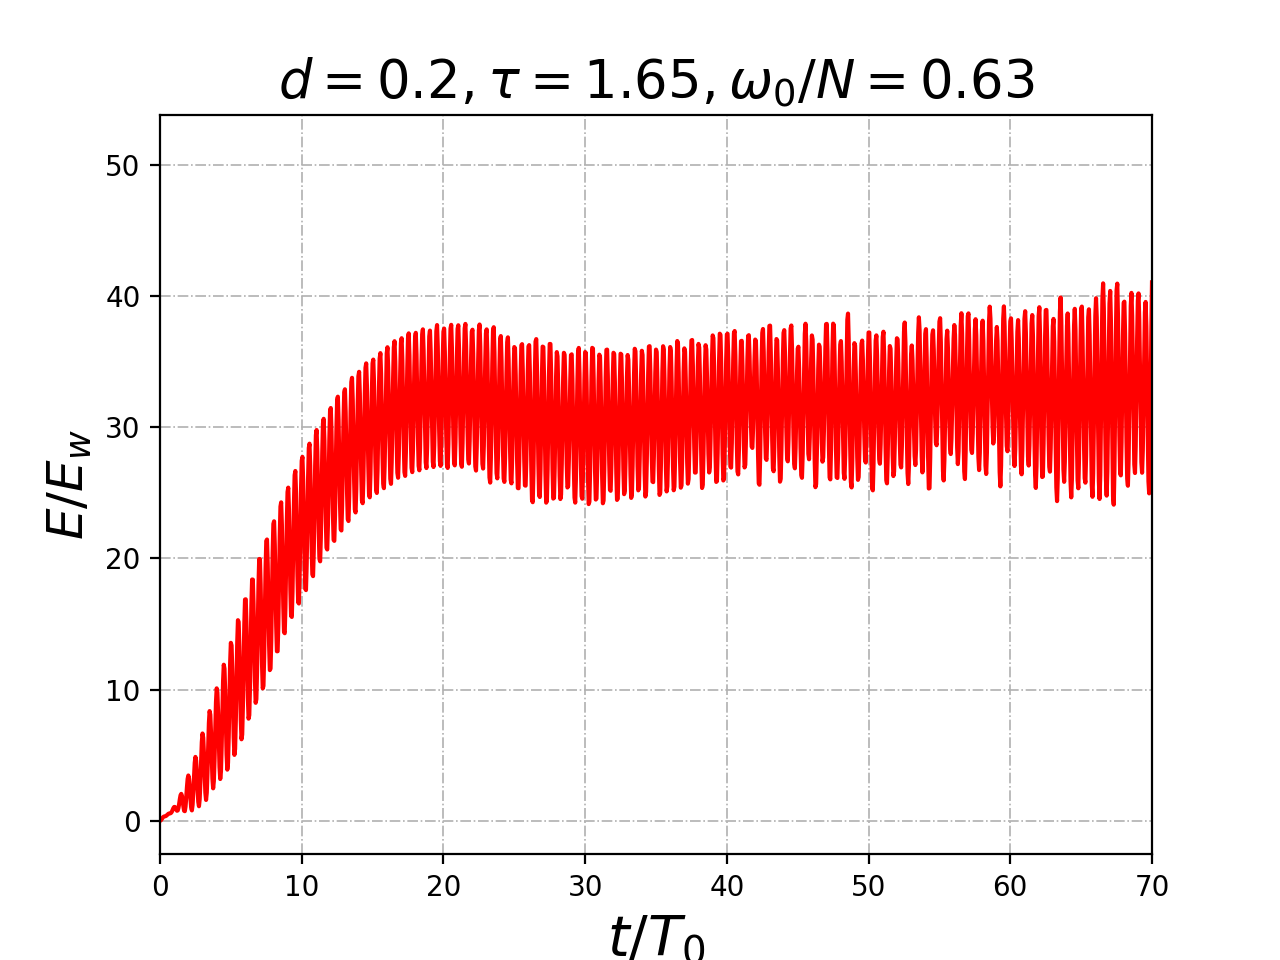
\includegraphics[width=1\textwidth]{pics/H40L60N1ap10dp20w0p63/2D36x36DiagramH40L60N1ap10dp20w0p63totKEnonDim.png}
	    \caption{Зависимость кинетической энергии от времени}
	\end{subfigure}
	\par
	\begin{subfigure}[с]{0.45\textwidth}
	    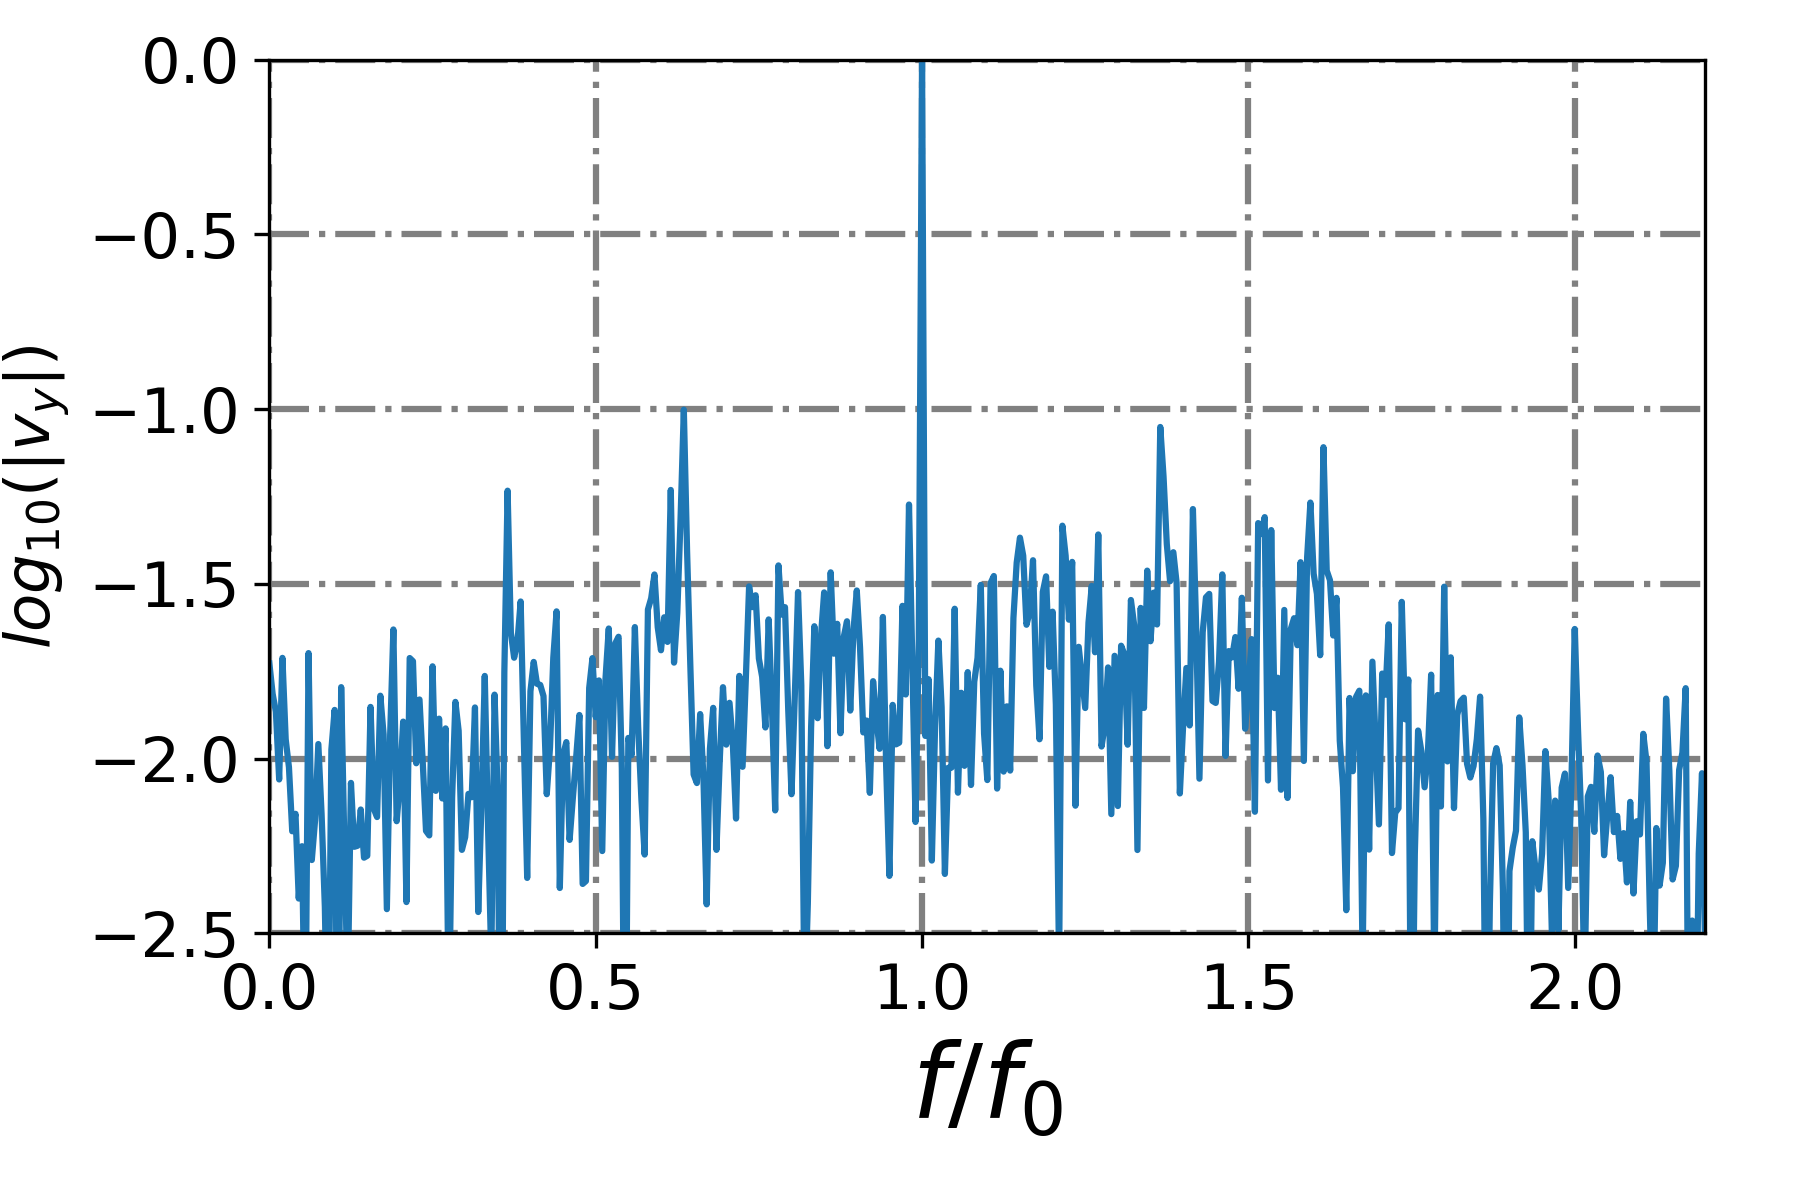
\includegraphics[width=1\textwidth]{pics/H40L60N1ap10dp20w0p63/spectrumX35p6Y11p2n4000.png}
	    \caption{Частотный спектр скорости}
	\end{subfigure}
	\begin{subfigure}[с]{0.45\textwidth}
	    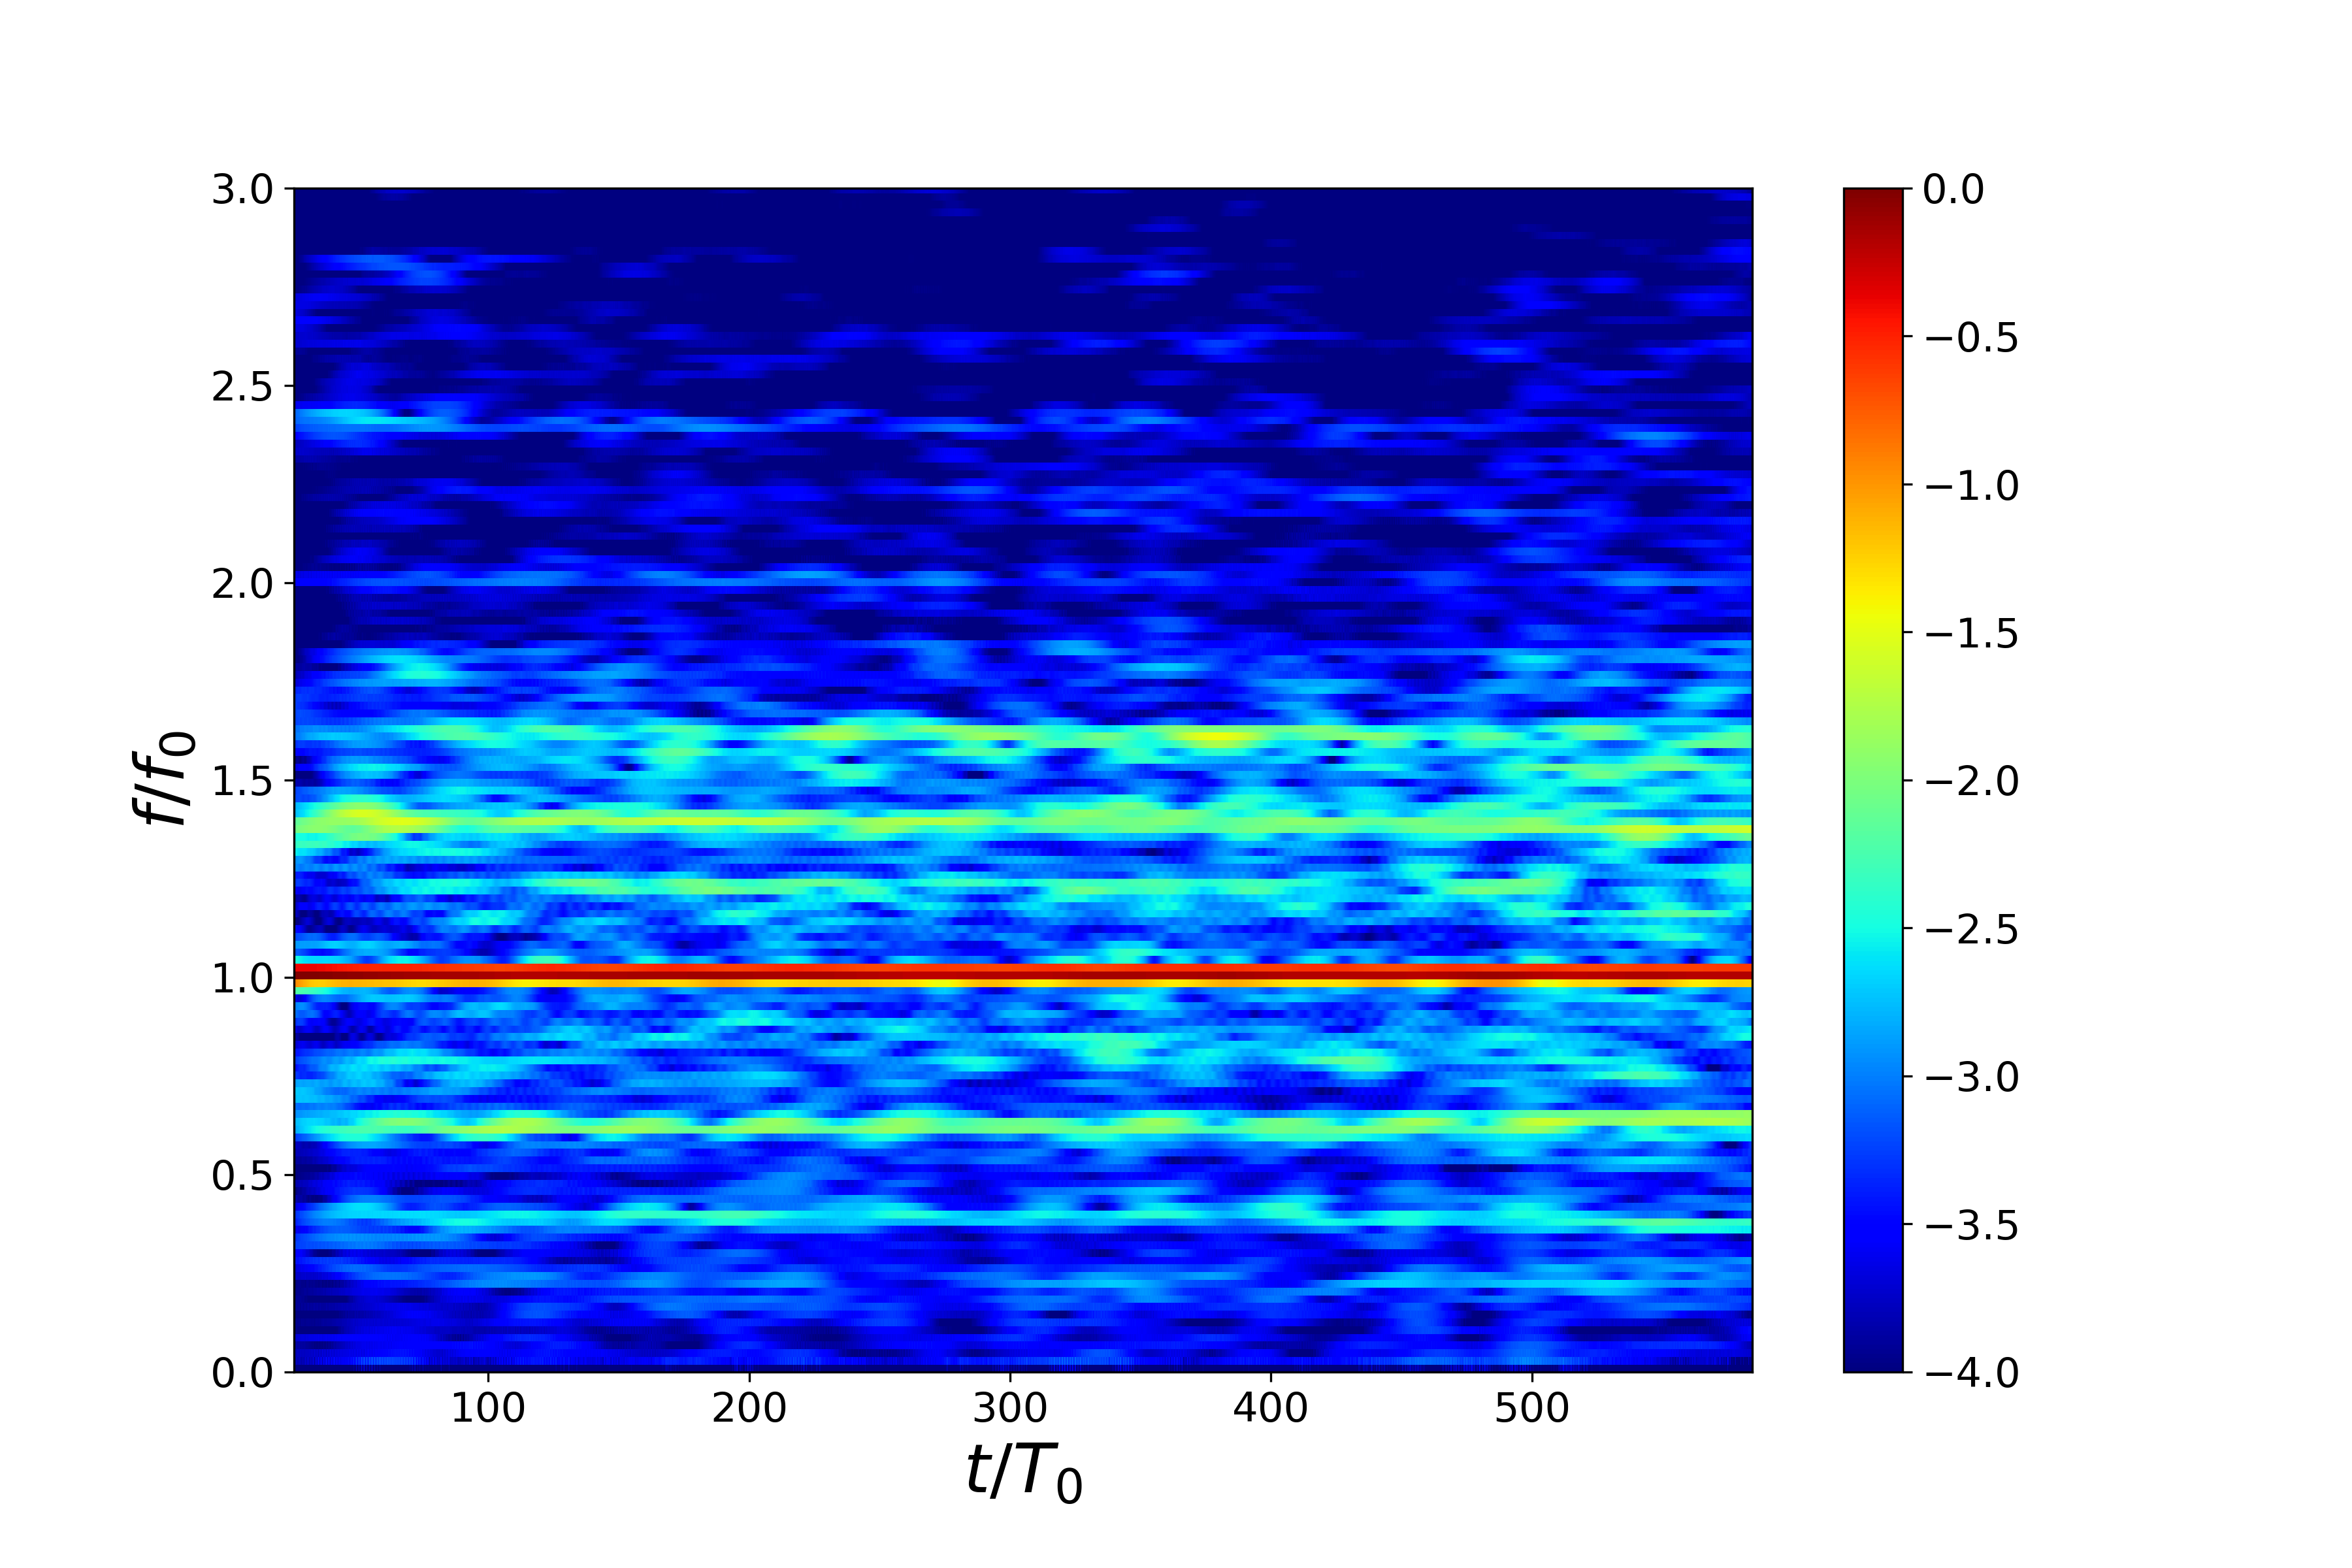
\includegraphics[width=1\textwidth]{pics/H40L60N1ap10dp20w0p63/TFspectrumX35p6Y11p2N1024.png}
	    \caption{Частотно-временная диаграмма}
	\end{subfigure}
	\label{fig:Vyamp1-1}
	\caption{Количественное исследования аттрактора с совпадающими частотами и образование неустойчивости}
	\label{fig:Vyamp1}
\end{figure}

Последующие режимы это попытка постепенно приблизить две частоты друг к другу и зафиксировать момент возникновения неустойчивости в зависимости от близости частот друг к другу. На рисунке \ref{fig:biharmVyap005-1} представлена картина течения при относительной разности частот в 0.05. При этом режиме наблюдаются дочерние волны как на изображении с вертикальной компонентой скорости, спектре так и на частотно временной диаграмме. При этом на последней наблюдаются  амплитудные <<всплески>>. Это объясняется совпадением фаз двух волновых процессов.

\begin{figure}
  \centering
  \begin{subfigure}[с]{0.45\textwidth}
    \includegraphics[width=1\textwidth]{pics/H40L60N1ap05dp20w1p63Deltawp05Biharm/2D36x36DiagramH40L60N1ap05dp20w0p63Deltawp3315BiharmVyn01019.png}
    \caption{Вертикальная компонента скорости при формировании аттрактора}
  \end{subfigure}
  \begin{subfigure}[с]{0.45\textwidth}
    \includegraphics[width=1\textwidth]{pics/H40L60N1ap05dp20w1p63Deltawp05Biharm/2D36x36DiagramH40L60N1ap05dp20w0p63Deltawp3315BiharmVyn04408.png}
    \caption{Вертикальная компонента скорости при установлении аттрактора}
  \end{subfigure}
  \par
  \begin{subfigure}[с]{0.45\textwidth}
    \includegraphics[width=1\textwidth]{pics/H40L60N1ap05dp20w1p63Deltawp05Biharm/vyX35p57Y11p27t4412.png}
    \caption{Вертикальная скорость}
  \end{subfigure}
  \begin{subfigure}[с]{0.45\textwidth}
    \includegraphics[width=1\textwidth]{pics/H40L60N1ap05dp20w1p63Deltawp05Biharm/2D36x36DiagramH40L60N1ap05dp20w1p63Deltawp05BiharmtotKEnonDim.png}
    \caption{Кинетическая энергия}
  \end{subfigure}
  \par
  \begin{subfigure}[с]{0.45\textwidth}
    \includegraphics[width=1\textwidth]{pics/H40L60N1ap05dp20w1p63Deltawp05Biharm/spectrumX35p6Y11p2.png}
    \caption{Спектр}
  \end{subfigure}
  \begin{subfigure}[с]{0.45\textwidth}
    \includegraphics[width=1\textwidth]{pics/H40L60N1ap05dp20w1p63Deltawp05Biharm/TFspectrumX35p6Y11p2N200.png}
    \caption{Частотно-временная диаграмма}
    \label{}
  \end{subfigure}
  \caption{Результаты количественного исследования характеристик течения стратифицированной жидкости в трапециевидном резервуаре при внешнем воздействии с двумя приближенными частотами $\omega_1/N=0.66$ $\omega_2/N=0.68$. Черной линией  на графиках вертикальной скорости и кинетической энергии показана огибающая амплитуды колебаний волнпородуктора.}

  \label{fig:biharmVyap005-1}
\end{figure}

С приближением частот друг к другу(см. рис. \ref{fig:biharmVyap005-2}) появляются дополнительные дочерние волны, но режим успевает стабилизироваться во временной промежуток разности фаз двух частот. 

\begin{figure}
  \centering
  \begin{subfigure}[с]{0.45\textwidth}
    \includegraphics[width=1\textwidth]{pics/H40L60N1ap05dp20w1p63Deltawp02Biharm/vyX35p57Y11p27t4400.png}
    \caption{Вертикальная компонента скорости в зависимости от времени}
  \end{subfigure}
  \begin{subfigure}[с]{0.45\textwidth}
    \includegraphics[width=1\textwidth]{pics/H40L60N1ap05dp20w1p63Deltawp02Biharm/2D36x36DiagramH40L60N1ap05dp20w1p63Deltawp02BiharmtotKEnonDim.png}
    \caption{Средняя кинетическая энергия в резервуаре в зависимости от времени}
  \end{subfigure}
  \par
  \begin{subfigure}[с]{0.45\textwidth}
    \includegraphics[width=1\textwidth]{pics/H40L60N1ap05dp20w1p63Deltawp02Biharm/spectrumX35p6Y11p2.png}
    \caption{Спектр}
  \end{subfigure}
  \begin{subfigure}[с]{0.45\textwidth}
    \includegraphics[width=1\textwidth]{pics/H40L60N1ap05dp20w1p63Deltawp02Biharm/TFspectrumX35p6Y11p2N256.png}
    \caption{Частотно-временная диаграмма}
  \end{subfigure}
  \caption{Количественные результаты исследования бигармонического аттрактора внутренних волн с двумя близкими частотами $\omega_1/N=0.628$,  $\omega_2/N=0.641$.}
  \label{fig:biharmVyap005-2}
\end{figure}

Помимо детального анализа результатов моделирования бигармонических аттракторов полученных с помощью метода спектральных элементов, были получены результаты моделирования с помощью метода конечного объема (см. рис. \ref{fig:biharm}). Из рисунка видно, что качественно картина течения совпала с предсказанной при помощи трассировки лучей. 

\begin{figure}
    \centering
    \scalebox{0.95}{
    \begin{tikzpicture}[scale=1.187, z={(-.707,-.5)}]
        \node[anchor=south west,inner sep=0] at (0,0) {\includegraphics[width=\textwidth]{pics/Biharm.png}};
        \draw (0,0,0) -- (12*0.98,0,0) -- (8*0.98,8*0.98,0)--(0,8*0.98,0) --cycle;
        \draw[style = dashed] (9*0.98,0,0)   -- (0,6.4*0.98,0) -- (2.0*0.98,8*0.98,0) -- (5.65*2*0.98,1.4*0.98,0)-- cycle;
        \draw[style = dashed] (0,0.985*2*0.98,0) -- (6.6*0.98,8*0.98,0) -- (9*0.98,6*0.98,0) -- (2.2*0.98,0,0)  -- cycle;
        \draw[thick,->] (9,6,0) -- (11.1,6,0) node[anchor=north east]{$x$};
        \draw[thick,->] (9,6,0) -- (9.1,8,0) node[anchor=north west]{$z$};
    \end{tikzpicture}
    }
    \caption{Поле горизонтальной компоненты скорости для бигармонического аттрактора и трассировка лучей.}
    \label{fig:biharm}
\end{figure}


\section{Кинетическая энергия для монохроматического и бигармонического режимов}

 Для геометрии, показанной на рис.\ref{fig:domainup}, нижняя и верхняя границы диапазона существования аттрактора соответствуют $\omega_{cr1}/N=0.55$ и $\omega_{cr2}/N=0.74$. При достижении этих критических значений частот происходит вырождение параллелограмма в диагональ трапеции. В качестве интегральной размерной меры эффективности генерации аттрактора при постоянной амплитуде волнопродуктора и неизменной форме резервуара принята кинетическая энергия жидкости, проинтегрированная по площади трапеции $S$: $E_{k}(t)=\int_{S}\frac{\rho_{m}}{2}\left[v_{y}^2(t)+v_{x}^2(t)\right]dS$. Для этой меры можно ввести значение, осредненное в скользящем временном окне по достаточно большому числу периодов колебаний $<E_{k}(t)>$, и вариацию относительно среднего, рассчитываемую как $r=D(E_{k}(t)-<E_{k}(t)>)/<E_{k}(t)>$, где $D(E_{k}(t)-<E_{k}(t)>)$ -- дисперсия относительно среднего. Безразмерные величины $\overline{E}_{k}(t)$ и $<\overline{E}_{k}(t)>$ определены путем нормировки на величину $\rho_{m}S(a\omega)^2/2$. Известно, что режимы движения в аттракторах могут быть близки как к прогрессивным, так и к стоячим волнам ~\cite{Brouzetetal2017}. Величина $r$ позволяет дать количественную оценку близости наблюдаемого режима к одному из этих предельных случаев \cite{Brouzetetal2017}. 


Характерный вид зависимостей, наблюдаемых в монохроматическом режиме при малой амплитуде колебаний показан на 

рис. \ref{fig:domainup}
для  $a=0.02$cм ($a/H=5\cdot 10^{-4}$), $\omega/N=0.63$. Характерное время выхода системы на установившийся режим составляет порядка $30$ периодов колебаний, спектр сигнала является с высокой точностью монохроматическим, колебания кинетической энергии относительно среднего имеют небольшую амплитуду ($r=0.103$). За первую ветвь аттрактора принят пучок с наибольшим значением плотности энергии, возникающий после фокусирующего отражения от наклонной стенки. Величины интегральных параметров, характеризующих линейные монохроматические режимы при фиксированном значении $a/H=5\cdot 10^{-4}$ в частотном диапазоне от $\omega_{cr1}/N=0.55$ до $\omega_{cr2}/N=0.74$ приведены в таблице \ref{tab:bolts002}. Видно, что при фиксированной амплитуде колебаний величина кинетической энергии аттрактора максимальна при $\omega/N=0.63$. Очевидно, что при этом значении частоты возмущающего воздействия следует ожидать сильных нелинейных эффектов при увеличении амплитуды колебаний волнопродуктора. Величина $r$ при $\omega/N=0.63$ достигает минимума: движение в аттракторе представлено прогрессивной волной.  Характерные картины течения и зависимости, наблюдаемые в случае слабонелинейного режима при $\omega/N=0.63$ приведены на рис.\ref{fig:Vyamp05} для $a=0.05$см ($a/H=1.25\cdot 10^{-3}$). В слабонелинейном режиме имеет место триадный резонанс \cite{Dauxoisetal2018}, при котором генерируются две дочерние субгармонические волны малой амплитуды.  Частотно-временная диаграмма, показанная на рис. \ref{fig:Vyamp05}, представляет собой спектр сигнала, вычисленный в скользящем окне и осредненный по окрестности точки, лежащей в середине первой ветви аттрактора. Частотный спектр внутренних волн при данном режиме является дискретным, с доминирующим вкладом, соответствующим частоте возмущения $\omega_{0}$, двумя дочерними субгармоническими частотами $\omega_{1}^{*}+\omega_{2}^{*}=\omega_{0}$, двумя супергармоническими частотам $\omega_{1}^{**}=\omega_{1}^{*}+\omega_{0}$, $\omega_{2}^{**}=\omega_{2}^{*}+\omega_{0}$ и удвоенной частотой $2\omega_{0}$. 


\begin{figure}
	\centering
	\begin{subfigure}[с]{0.45\textwidth}
	    \includegraphics[width=1\textwidth]{pics/H40L60N1ap05dp20w0p63/2D36x36DiagramH40L60N1ap05dp20w0p63Vyn00308.png}
	    \caption{Поле вертикальной компоненты скорости при монохроматическом внешнем воздействии с амплитудой($a/H=5\cdot 10^{-4}$)}
	\end{subfigure}
	\begin{subfigure}[с]{0.45\textwidth}
	    \includegraphics[width=1\textwidth]{pics/H40L60N1ap05dp20w0p63/2D36x36DiagramH40L60N1ap05dp20w0p63Pn00308.png}
	    \caption{Поле давления при монохроматическом внешнем воздействии с амплитудой ($a/H=5\cdot 10^{-4}$)}
	\end{subfigure}
	\par
	\begin{subfigure}[с]{0.45\textwidth}
	    \includegraphics[width=1\textwidth]{pics/H40L60N1ap05dp20w0p63/vyX35p57Y11p27t4400.png}
	    \caption{Скорость в середине первого луча аттрактора}
	\end{subfigure}
	\begin{subfigure}[с]{0.45\textwidth}
	    \includegraphics[width=1\textwidth] {pics/H40L60N1ap05dp20w0p63/2D36x36DiagramH40L60N1ap05dp20w0p63totKEnonDim.png}
	    \caption{Кинетическая энергия в середине первого луча аттрактора}
	\end{subfigure}
	\par
	\begin{subfigure}[с]{0.45\textwidth}
	    \includegraphics[width=1\textwidth]{{pics/H40L60N1ap05dp20w0p63/spectrumX35.6Y11.2}.png}
	    \caption{Спектр}
	\end{subfigure}
	\begin{subfigure}[с]{0.45\textwidth}
	    \includegraphics[width=1\textwidth]{{pics/H40L60N1ap05dp20w0p63/TFspectrumX35.6Y11.2N1024}.png}
	    \caption{Частотно-временная диаграмма}
	\end{subfigure}
	\caption{Характерная картина течения при монохроматическом воздействии }
	\label{fig:Vyamp05}
\end{figure}

\begin{table}
	\caption{ Кинетическая энергия при монохроматических воздействиях с амплитудой $a=0.02 cm$}. 
	\begin{center}
		\begin{tabular}{|c|c|c|c|c|c|}
			\hline
			$\displaystyle \frac{\omega_0}{N}$ & $E_k $ &  $<\overline{E}_{k}>$ & r\\
			0.55 ($\omega_{cr,1}$) & $1.32 \cdot 10^{-4}   $& 2.151    & 0.618     \\
			0.58                   & $8.45 \cdot 10^{-4}   $& 12.56    & 0.281     \\
			0.59                   & $ 12  \cdot 10^{-4}   $& 17.33    & 0.3       \\
			0.63                   & $29   \cdot 10^{-4}   $& 36.68    & 0.103     \\
			0.641                  & $23   \cdot 10^{-4}   $& 28.55    & 0.1129    \\
			0.66                   & $13.2 \cdot 10^{-4}   $& 15.14    & 0.152     \\
			0.70                   & $2.84 \cdot 10^{-4}   $& 2.896    & 0.295     \\
			0.74 ($\omega_{cr,2}$) & $1.50 \cdot 10^{-4}   $& 1.356    & 0.215     \\
			\hline
		\end{tabular}
	\end{center}
	\label{tab:bolts002}
\end{table}

При дальнейшем увеличении амплитуды возмущения до $a=0.1$см ($a/H=2.5\cdot 10^{-3}$) происходит развитие каскада триадных взаимодействий. Характерные картины волновых полей, спектров и развития во времени процесса колебаний и кинетической энергии системы приведены на рисунках \ref{fig:Vyamp1}. В частотном спектре сигнала доминируют дискретные компоненты, соответствующие частотам дочерних волн, возникающих при триадном резонансе аналогичные компонентам спектра, возникающим в слабонелинейном случае ($a/H=1.25\cdot 10^{-3}$). При этом полный спектр сигнала представляет собой суперпозицию дискретного и непрерывного спектра. Наличие непрерывного спектра свидетельствует о возникновении режима развитой волновой турбулентности \cite{Brouzet2016,Brouzetetal2017}. Соответствующие характеристики для кинетической энергии системы в сильно нелинейном режиме приведены в таблице \ref{tab:bolts01}. Из сопоставления таблиц \ref{tab:bolts002} и \ref{tab:bolts01} видно, что величины глобальных безразмерных энергетических характеристик системы (средней энергии  $<\overline{E}_{k}>$ и вариации относительно среднего $r$) в случае режима развитой волновой турбулентности слабо отличаются от безразмерных величин, характерных для линейного режима. Сопоставление волновых картин в линейном и нелинейном случаях показывает, что во втором случае энергия более равномерно распределена по изучаемой области: ветви аттрактора имеют большую ширину, а дочерние волны заполняют все пространство.

\begin{table}
	\caption{  Кинетическая энергия при монохроматических воздействиях с амплитудной $a=0.1 cm$. }
	\begin{center}
		\begin{tabular}{|c|c|c|c|c|}
			\hline
			$\displaystyle \frac{\omega_0}{N}$ & $E_k (erg)$ &  $<\overline{E}_{k}>$  & r\\
			%          $a$ &    $\displaystyle \frac{\omega_0}{N}$   & $E_k$ & ${E_k}/{\frac{(a\omega_0)^2}{2}}$ & $D_k$ & r\\
			0.55 ($\omega_{cr,1}$) & $33.0 \cdot 10^{-4}              $& 2.14  & 0.6193     \\
			0.63                   & $725 \cdot 10^{-4}              $& 36.7  & 0.1346     \\
			0.74 ($\omega_{cr,2}$) & $37.0 \cdot 10^{-4}              $& 1.35  & 0.2192     \\
			\hline
		\end{tabular}
	\end{center}
	\label{tab:bolts01}
\end{table}

Характерный пример волновой картины и основных качественных и количественных характеристик системы в линейном случае при бигармоническом внешнем воздействии приведен на рис.\ref{fig:biharmVyamp02} для следующих значений параметров: $\omega_1/N=0.58, \omega_2/N=0.66, a=0.02$см. Видно, что система выходит на режим квазистационарных биений за время порядка $40$ периодов колебаний, что близко к характерному времени выхода на процесс стационарных колебаний в монохроматическом случае. На частотном спектре доминируют пики, соответствующие частотам внешнего возмущения, имеются также пики, соответствующие частоте  $2\omega_1/N$ и разностной частоте $(\omega_2-\omega_1)/N$, но их величина более чем на два порядка меньше основного пика. Моменты времени, соответствующие максимальным значениям кинетической энергии, существенно отстают от моментов времени, соответствующих максимальным значениям амплитуды колебаний волнпродуктора. Важно отметить, что после выхода системы на режим установившихся биений средняя кинетическая энергия системы, возбуждаемой бигармоническим возмущением, с высокой точностью равна сумме энергий аттракторов, возбуждаемых монохроматическими возмущениями по отдельности $\overline{E}_{k}= { 21.7 \cdot 10^{-4}  }\approx \overline{E}_{k1}+\overline{E}_{k2}= (8.45+13.2) \cdot 10^{-4} = 21.65 \cdot 10^{-4}\, (erg/cm^2) $. Таким образом, в линейном режиме с высокой точностью соблюдается принцип линейной суперпозиции, что выполняется также при малой разности частот $(\omega_1-\omega_2)/N$. 

Примеры нелинейной динамики волновых аттракторов, генерируемых бигармоническими колебаниями волнопродуктора приведены на рис. \ref{fig:biharmVyap005-1} %\ref{fig:biharmVyap005-1-1} 
($\omega_1/N=0.66$, $\omega_2/N=0.628$, $\delta \omega/N=0.031$) и \ref{fig:biharmVyap005-2}, 
%\ref{fig:biharmVyap005-2-1} 
($\omega_1/N=0.628$, $\omega_2/N=0.641$, $\delta \omega/N=0.013$). Во всех случаях амплитуды колебаний волнопродуктора составили $a_{1}=a_{2}=0.05$см. Можно видеть, что в обоих случаях формируется движение, для которого характерен сложный частотный спектр, причем при уменьшении расстройки частот $\delta \omega$ наблюдается тенденция к более густому <<заселению>> спектра.  На графиках зависимости вертикальной скорости от времени виден характерный процесс <<биений>>. График зависимости кинетической энергии системы от времени показывает, что помимо колебаний среднего значения энергии имеет место нетривиальная динамика высокочастотных пульсаций энергии: на фазах роста и убывания огибающей амплитуды колебаний волнопродуктора амплитуды пульсаций могут отличаться на порядок. Таким образом, для нелинейного бигармонического режима характерны периодические <<вспышки>> волновой турбулентности. Такие <<вспышки>> хорошо видны на частотно-временных диаграммах, приведенных на рис.  \ref{fig:biharmVyap005-1} и \ref{fig:biharmVyap005-2}. В частности, на частотно-вереиенной диаграмме, приведенной на рис.  \ref{fig:biharmVyap005-1}, можно видеть, что <<биения>> амплитуды сигнала на частоте, близкой к частоте возмущающего воздействия, сдвинуты по времени относительно <<биений>> дочерних волн. Таким образом, <<биения>> огибающей колебаний волнопродуктора, <<биения>> средней кинетической энергии и <<вспышки>> волновой турбулентности рассогласованны между собой по времени. Можно предположить, что и в природных системах имеется рассогласование по времени между огибающей амплитуды внутреннего прилива и интенсификацией внутренней волновой турбулентности и перемешивания. Предварительное исследование энергии аттракторов, генерируемых бигармоническим возмущением, показывает, что в нелинейном случае средняя энергия системы существенным образом отличается от суммы энергий составляющих.  

\section*{Заключение к главе 3}

Для определения наиболее интересного диапазона параметров выполнено подробное исследование генерации аттракторов при монохроматическом возмущении, в результате чего определен частотный диапазон, в котором генерация аттракторов наиболее эффективна. Исследование поведения аттракторов при бигармоническом внешнем воздействии показало, что в линейном случае справедлив принцип суперпозиции: аттракторы, генерируемые каждой из компонент бигармонического возмущения практически не взаимодействуют друг с другом. В нелинейном случае при бигармоническом внешнем воздействии наблюдается режим биений, сопровождающийся вспышками волновой турбулентности, возникающей вследствие каскада триадных взаимодействий. При этом уровень пульсаций кинетической энергии на фазе роста огибающей амплитуды волнопродуктора, может на порядок превышать уровень, соответствующий спаду амплитуды колебаний волнопродуктора. 

\chapter*{Заключение}
\label{cha:Conclusion}

%Заключение последовательное логически стройное изложение итогов исследования в соответствии с целью и задачами, поставленными и сформулированными во введении. В нем содержатся выводы и определяются дальнейшие перспективы работы.

% \begin{itemize}
%     \item В ходе работы определена целесообразность использования метода конечного объема для моделирования аттракторов внутренних волн.
%     \item Найдены теоретические диапазоны частот колебаний волнопродуктора, которые способны порождать аттракторы.
%     \item Установлено, что при воздействии на резервуар со стратифицированной жидкостью волнопродуктором, который совершает колебания описываемые суммой двух монохроматических функций образуется суперпозиция двух аттракторов в одном резервуаре.
%     \item Обнаружено, что при близости частот двух монохроматических функций возбуждающих внутренние волны в резервуаре образуются амплитудные биения. 
% \end{itemize}



Показано, что результаты моделирования аттракторов внутренних волн, полученные с помощью методов конечного объёма при увеличении количества ячеек стремятся к результатам, полученным с помощью метода высокого порядка. Таким образом сделан вывод о целесообразности дальнейшего использования конечно объёмной реализации квазигидродинамических уравнений для моделирования аттракторов внутренних волн. 
Аналитически определены  границы частотного диапазона существования аттрактора. Выведены формулы расчёта каждой из границ в зависимости от геометрических характеристик резервуара и частоты плавучести.


Получены результаты моделирования бигармонических аттракторов, то есть таких, которые возникают при воздействии на жидкость в трапециевидном резервуаре с двумя частотами, попадающими в интервал существования аттрактора. Установлено, что в этом случае картина течения каждой частоты по отдельности накладывается друг на друга. В резервуаре появляются два независимых аттрактора, каждый из которых совершает движение с собственной частотой, а взаимодействуют они только в точках пересечения. 


Рассмотрены различные комбинации частот из диапазона существования аттракторов. Когда частоты совпадают, это фактически удваивает амплитуду колебаний волнопродуктора монохроматического аттрактора. В случае большой амплитуды колебаний волнопродуктора аттрактор начинает поражать дочерние волны и насыщает спектр. В случае разнесённых частот аттракторы практически не взаимодействуют, амплитуды не складываются. В случае, когда частоты приближены друг к другу, в момент совпадения фаз наблюдается взаимодействие аттракторов, тогда постепенно спектр частот начинает насыщаться, но в момент разности фаз спектр возвращается в исходное состояние. В случае, когда частоты располагаются еще ближе друг к другу, на частотно-временной диаграмме наблюдается еще более активное взаимодействие аттракторов, а на графике зависимости средней кинетической энергии в резервуаре от времени наблюдаются биения.


Выяснено, что с большой точностью сумма средних кинетических энергий аттракторов, образующихся при монохроматическом режиме колебаний волнопродуктора, равна средней кинетической энергии бигармонического аттрактора.

Работа представляет собой первый шаг к моделированию аттракторов как природного явления в океане. Для этого необходимо разработать инструменты численного моделирования монохроматического аттрактора в условиях геометрии, приближенной к реальной. А также исследовать течения возникающие при воздействии на стратифицированную жидкость суммой нескольких монохроматических колебаний. 

Для реализации инструмента численного моделирования в сложной геометрии была разработана программа, которая подлежала государственной регистрации номер 2018663951. Разработанный инструмент имеет ряд преимуществ относительно уже существующих программных средств, такие как точность, гибкость, возможность встроить дополнительные модули физических процессов и возможность работать со сложной геометрией на неортогональных сетках. Количественное соответствие результатов моделирования методом конечного объема и методом спектральных элементов показывают целесообразность дальнейшего развития метода конечного объема на базе квазигидродинамических уравнений. Соответствие предсказанной трассировкой лучей формы бигармонического аттрактора и результатов моделирования с помощью регуляризованных уравнений дает возможность сделать заключение о целесообразности дальнейшего применения. 

Количественное исследование показало, что после выхода системы на режим установившихся колебаний средняя кинетическая энергия системы, возбуждаемой бигармоническим возмущением, с высокой точностью равна сумме энергий аттракторов, возбуждаемых монохроматическими возмущениями по отдельности. Таким образом, в линейном режиме с высокой точностью соблюдается принцип линейной суперпозиции, что выполняется также при малой разности частот. 

В нелинейном случае средняя энергия системы существенным образом отличается от суммы энергий составляющих. Наблюдается режим <<биений>> сопровождающийся <<вспышками>> волновой турбулентности, возникающей вследствие каскада триадных взаимодействий. При этом уровень пульсаций кинетической
энергии на фазе роста огибающей амплитуды волнопродуктора, может на порядок превышать уровень, соответствующий спаду амплитуды колебаний волнопродуктора.

Реализован квазигидродинамический подход на базе конечно объёмного пакета OpenFOAM. Программа охватывает дозвуковой и трансзвуковой диапазон скоростей, позволяет проводить численное моделирование вязких течений с переносом. Исходный код, тестовые примеры и документация размещена в открытом хранилище исходного кода на github. 

% % Список литературы при помощи BibTeX
% Юзать так:
%
% pdflatex rpz
% bibtex rpz
% pdflatex rpz

%\bibliographystyle{gost780u}
%\bibliographystyle{plain}
%\bibliographystyle{ugost2008ns}
\bibliographystyle{ugost2008}
\bibliography{rpz}

%%% Local Variables: 
%%% mode: latex
%%% TeX-master: "rpz"
%%% End: 

%% % Список литературы при помощи BibTeX
% Юзать так:
%
% pdflatex rpz
% bibtex rpz
% pdflatex rpz

%\bibliographystyle{gost780u}
%\bibliographystyle{plain}
%\bibliographystyle{ugost2008ns}
\bibliographystyle{ugost2008}
\bibliography{rpz}

%%% Local Variables: 
%%% mode: latex
%%% TeX-master: "rpz"
%%% End: 


%\appendix   % Тут идут приложения

\end{document}

%%% Local Variables:
%%% mode: latex
%%% TeX-master: t
%%% End:
